%%%%%%%%%%%%%%%%%%%%%%%%%%%%%%%%%%%%%%%%%%%%%%%%%%%%%%%%%%%%%%%%%%%%%%
% Template for a UBC-compliant dissertation
% At the minimum, you will need to change the information found
% after the "Document meta-data"
%
%!TEX TS-program = pdflatex
%!TEX encoding = UTF-8 Unicode

%% The ubcdiss class provides several options:
%%   gpscopy (aka fogscopy)
%%       set parameters to exactly how GPS specifies
%%         * single-sided
%%         * page-numbering starts from title page
%%         * the lists of figures and tables have each entry prefixed
%%           with 'Figure' or 'Table'
%%       This can be tested by `\ifgpscopy ... \else ... \fi'
%%   10pt, 11pt, 12pt
%%       set default font size
%%   oneside, twoside
%%       whether to format for single-sided or double-sided printing
%%   balanced
%%       when double-sided, ensure page content is centred
%%       rather than slightly offset (the default)
%%   singlespacing, onehalfspacing, doublespacing
%%       set default inter-line text spacing; the ubcdiss class
%%       provides \textspacing to revert to this configured spacing
%%   draft
%%       disable more intensive processing, such as including
%%       graphics, etc.
%%

% For submission to GPS
\documentclass[gpscopy,onehalfspacing,11pt]{ubcdiss}

% For your own copies (looks nicer)
% \documentclass[balanced,twoside,11pt]{ubcdiss}

%%%%%%%%%%%%%%%%%%%%%%%%%%%%%%%%%%%%%%%%%%%%%%%%%%%%%%%%%%%%%%%%%%%%%%
%%%%%%%%%%%%%%%%%%%%%%%%%%%%%%%%%%%%%%%%%%%%%%%%%%%%%%%%%%%%%%%%%%%%%%
%%
%% FONTS:
%% 
%% The defaults below configures Times Roman for the serif font,
%% Helvetica for the sans serif font, and Courier for the
%% typewriter-style font.  Configuring fonts can be time
%% consuming; we recommend skipping to END FONTS!
%% 
%% If you're feeling brave, have lots of time, and wish to use one
%% your platform's native fonts, see the commented out bits below for
%% XeTeX/XeLaTeX.  This is not for the faint at heart. 
%% (And shouldn't you be writing? :-)
%%

%% NFSS font specification (New Font Selection Scheme)
\usepackage{times,mathptmx,courier}
\usepackage[scaled=.92]{helvet}

%% Math or theory people may want to include the handy AMS macros
%\usepackage{amssymb}
%\usepackage{amsmath}
%\usepackage{amsfonts}

%% The pifont package provides access to the elements in the dingbat font.   
%% Use \ding{##} for a particular dingbat (see p7 of psnfss2e.pdf)
%%   Useful:
%%     51,52 different forms of a checkmark
%%     54,55,56 different forms of a cross (saltyre)
%%     172-181 are 1-10 in open circle (serif)
%%     182-191 are 1-10 black circle (serif)
%%     192-201 are 1-10 in open circle (sans serif)
%%     202-211 are 1-10 in black circle (sans serif)
%% \begin{dinglist}{##}\item... or dingautolist (which auto-increments)
%% to create a bullet list with the provided character.
\usepackage{pifont}

%%%%%%%%%%%%%%%%%%%%%%%%%%%%%%%%%%%%%%%%%%%%%%%%%%%%%%%%%%%%%%%%%%%%%%
%% Configure fonts for XeTeX / XeLaTeX using the fontspec package.
%% Be sure to check out the fontspec documentation.
%\usepackage{fontspec,xltxtra,xunicode}	% required
%\defaultfontfeatures{Mapping=tex-text}	% recommended
%% Minion Pro and Myriad Pro are shipped with some versions of
%% Adobe Reader.  Adobe representatives have commented that these
%% fonts can be used outside of Adobe Reader.
%\setromanfont[Numbers=OldStyle]{Minion Pro}
%\setsansfont[Numbers=OldStyle,Scale=MatchLowercase]{Myriad Pro}
%\setmonofont[Scale=MatchLowercase]{Andale Mono}

%% Other alternatives:
%\setromanfont[Mapping=tex-text]{Adobe Caslon}
%\setsansfont[Scale=MatchLowercase]{Gill Sans}
%\setsansfont[Scale=MatchLowercase,Mapping=tex-text]{Futura}
%\setmonofont[Scale=MatchLowercase]{Andale Mono}
%\newfontfamily{\SYM}[Scale=0.9]{Zapf Dingbats}
%% END FONTS
%%%%%%%%%%%%%%%%%%%%%%%%%%%%%%%%%%%%%%%%%%%%%%%%%%%%%%%%%%%%%%%%%%%%%%
%%%%%%%%%%%%%%%%%%%%%%%%%%%%%%%%%%%%%%%%%%%%%%%%%%%%%%%%%%%%%%%%%%%%%%



%%%%%%%%%%%%%%%%%%%%%%%%%%%%%%%%%%%%%%%%%%%%%%%%%%%%%%%%%%%%%%%%%%%%%%
%%%%%%%%%%%%%%%%%%%%%%%%%%%%%%%%%%%%%%%%%%%%%%%%%%%%%%%%%%%%%%%%%%%%%%
%%
%% Recommended packages
%%
\usepackage{checkend}	% better error messages on left-open environments
\usepackage{graphicx}	% for incorporating external images

%% booktabs: provides some special commands for typesetting tables as used
%% in excellent journals.  Ignore the examples in the Lamport book!
\usepackage{booktabs}

%% listings: useful support for including source code listings, with
%% optional special keyword formatting.  The \lstset{} causes
%% the text to be typeset in a smaller sans serif font, with
%% proportional spacing.
\usepackage{listings}
\lstset{basicstyle=\sffamily\scriptsize,showstringspaces=false,fontadjust}

%% The acronym package provides support for defining acronyms, providing
%% their expansion when first used, and building glossaries.  See the
%% example in glossary.tex and the example usage throughout the example
%% document.
%% NOTE: to use \MakeTextLowercase in the \acsfont command below,
%%   we *must* use the `nohyperlinks' option -- it causes errors with
%%   hyperref otherwise.  See Section 5.2 in the ``LaTeX 2e for Class
%%   and Package Writers Guide'' (clsguide.pdf) for details.
\usepackage[printonlyused,nohyperlinks]{acronym}

%% The ubcdiss.cls loads the `textcase' package which provides commands
%% for upper-casing and lower-casing text.  The following causes
%% the acronym package to typeset acronyms in small-caps
%% as recommended by Bringhurst.
\renewcommand{\acsfont}[1]{{\scshape \MakeTextLowercase{#1}}}

%% color: add support for expressing colour models.  Grey can be used
%% to great effect to emphasize other parts of a graphic or text.
%% For an excellent set of examples, see Tufte's "Visual Display of
%% Quantitative Information" or "Envisioning Information".
\usepackage{color}
\definecolor{greytext}{gray}{0.5}

%% comment: provides a new {comment} environment: all text inside the
%% environment is ignored.
%%   \begin{comment} ignored text ... \end{comment}
\usepackage{comment}

%% The natbib package provides more sophisticated citing commands
%% such as \citeauthor{} to provide the author names of a work,
%% \citet{} to produce an author-and-reference citation,
%% \citep{} to produce a parenthetical citation.
%% We use \citeeg{} to provide examples
%\usepackage[numbers,sort&compress]{natbib}
\usepackage[round]{natbib}
\newcommand{\citeeg}[1]{\citep[e.g.,][]{#1}}

%% The titlesec package provides commands to vary how chapter and
%% section titles are typeset.  The following uses more compact
%% spacings above and below the title.  The titleformat that follow
%% ensure chapter/section titles are set in singlespace.
\usepackage[compact]{titlesec}
\titleformat*{\section}{\singlespacing\raggedright\bfseries\Large}
\titleformat*{\subsection}{\singlespacing\raggedright\bfseries\large}
\titleformat*{\subsubsection}{\singlespacing\raggedright\bfseries}
\titleformat*{\paragraph}{\singlespacing\raggedright\itshape}

%% The caption package provides support for varying how table and
%% figure captions are typeset.
\usepackage[format=hang,indention=-1cm,labelfont={bf},margin=1em]{caption}

%% url: for typesetting URLs and smart(er) hyphenation.
%% \url{http://...} 
\usepackage{url}
\urlstyle{sf}	% typeset urls in sans-serif


%%%%%%%%%%%%%%%%%%%%%%%%%%%%%%%%%%%%%%%%%%%%%%%%%%%%%%%%%%%%%%%%%%%%%%
%%%%%%%%%%%%%%%%%%%%%%%%%%%%%%%%%%%%%%%%%%%%%%%%%%%%%%%%%%%%%%%%%%%%%%
%%
%% Possibly useful packages: you may need to explicitly install
%% these from CTAN if they aren't part of your distribution;
%% teTeX seems to ship with a smaller base than MikTeX and MacTeX.
%%
%\usepackage{pdfpages}	% insert pages from other PDF files
%\usepackage{longtable}	% provide tables spanning multiple pages
%\usepackage{chngpage}	% support changing the page widths on demand
%\usepackage{tabularx}	% an enhanced tabular environment

%% enumitem: support pausing and resuming enumerate environments.
%\usepackage{enumitem}

%% rotating: provides two environments, sidewaystable and sidewaysfigure,
%% for typesetting tables and figures in landscape mode.  
%\usepackage{rotating}

%% subfig: provides for including subfigures within a figure,
%% and includes being able to separately reference the subfigures.
%\usepackage{subfig}

%% ragged2e: provides several new new commands \Centering, \RaggedLeft,
%% \RaggedRight and \justifying and new environments Center, FlushLeft,
%% FlushRight and justify, which set ragged text and are easily
%% configurable to allow hyphenation.
%\usepackage{ragged2e}

%% The ulem package provides a \sout{} for striking out text and
%% \xout for crossing out text.  The normalem and normalbf are
%% necessary as the package messes with the emphasis and bold fonts
%% otherwise.
%\usepackage[normalem,normalbf]{ulem}    % for \sout

%%%%%%%%%%%%%%%%%%%%%%%%%%%%%%%%%%%%%%%%%%%%%%%%%%%%%%%%%%%%%%%%%%%%%%
%% HYPERREF:
%% The hyperref package provides for embedding hyperlinks into your
%% document.  By default the table of contents, references, citations,
%% and footnotes are hyperlinked.
%%
%% Hyperref provides a very handy command for doing cross-references:
%% \autoref{}.  This is similar to \ref{} and \pageref{} except that
%% it automagically puts in the *type* of reference.  For example,
%% referencing a figure's label will put the text `Figure 3.4'.
%% And the text will be hyperlinked to the appropriate place in the
%% document.
%%
%% Generally hyperref should appear after most other packages

%% The following puts hyperlinks in very faint grey boxes.
%% The `pagebackref' causes the references in the bibliography to have
%% back-references to the citing page; `backref' puts the citing section
%% number.  See further below for other examples of using hyperref.
%% 2009/12/09: now use `linktocpage' (Jacek Kisynski): GPS now prefers
%%   that the ToC, LoF, LoT place the hyperlink on the page number,
%%   rather than the entry text.


%% !!!!!! Jes changed this to previous version !!!!!!!

\usepackage[bookmarks,bookmarksnumbered,%
citebordercolor={0.8 0.8 0.8},filebordercolor={0.8 0.8 0.8},%
linkbordercolor={0.8 0.8 0.8},pagebordercolor={0.8 0.8 0.8},%
urlbordercolor={0.8 0.8 0.8},%
%%    allbordercolors={0.8 0.8 0.8},%
    pagebackref,linktocpage%
    ]{hyperref}


%% The following change how the the back-references text is typeset in a
%% bibliography when `backref' or `pagebackref' are used
\renewcommand\backrefpagesname{\(\rightarrow\) pages}
\renewcommand\backref{\textcolor{greytext} \backrefpagesname\ }

%% The following uses most defaults, which causes hyperlinks to be
%% surrounded by colourful boxes; the colours are only visible in
%% PDFs and don't show up when printed:
%\usepackage[bookmarks,bookmarksnumbered]{hyperref}

%% The following disables the colourful boxes around hyperlinks.
%\usepackage[bookmarks,bookmarksnumbered,pdfborder={0 0 0}]{hyperref}

%% The following disables all hyperlinking, but still enabled use of
%% \autoref{}
%\usepackage[draft]{hyperref}

%% The following commands causes chapter and section references to
%% uppercase the part name.
\renewcommand{\chapterautorefname}{Chapter}
\renewcommand{\sectionautorefname}{Section}
\renewcommand{\subsectionautorefname}{Section}
\renewcommand{\subsubsectionautorefname}{Section}

%% If you have long page numbers (e.g., roman numbers in the 
%% preliminary pages for page 28 = xxviii), you might need to
%% uncomment the following and tweak the \@pnumwidth length
%% (default: 1.55em).  See the tocloft documentation at
%% http://www.ctan.org/tex-archive/macros/latex/contrib/tocloft/
% \makeatletter
% \renewcommand{\@pnumwidth}{3em}
% \makeatother

%%%%%%%%%%%%%%%%%%%%%%%%%%%%%%%%%%%%%%%%%%%%%%%%%%%%%%%%%%%%%%%%%%%%%%
%%%%%%%%%%%%%%%%%%%%%%%%%%%%%%%%%%%%%%%%%%%%%%%%%%%%%%%%%%%%%%%%%%%%%%
%%
%% Some special settings that controls how text is typeset
%%
% \raggedbottom		% pages don't have to line up nicely on the last line
% \sloppy		% be a bit more relaxed in inter-word spacing
% \clubpenalty=10000	% try harder to avoid orphans
% \widowpenalty=10000	% try harder to avoid widows
% \tolerance=1000

%% And include some of our own useful macros
% This file provides examples of some useful macros for typesetting
% dissertations.  None of the macros defined here are necessary beyond
% for the template documentation, so feel free to change, remove, and add
% your own definitions.
%
% We recommend that you define macros to separate the semantics
% of the things you write from how they are presented.  For example,
% you'll see definitions below for a macro \file{}: by using
% \file{} consistently in the text, we can change how filenames
% are typeset simply by changing the definition of \file{} in
% this file.
% 
%% The following is a directive for TeXShop to indicate the main file
%%!TEX root = diss.tex

\newcommand{\NA}{\textsc{n/a}}	% for "not applicable"
\newcommand{\eg}{e.g.,\ }	% proper form of examples (\eg a, b, c)
\newcommand{\ie}{i.e.,\ }	% proper form for that is (\ie a, b, c)
\newcommand{\etal}{\emph{et al}}

% Some useful macros for typesetting terms.
\newcommand{\file}[1]{\texttt{#1}}
\newcommand{\class}[1]{\texttt{#1}}
\newcommand{\latexpackage}[1]{\href{http://www.ctan.org/macros/latex/contrib/#1}{\texttt{#1}}}
\newcommand{\latexmiscpackage}[1]{\href{http://www.ctan.org/macros/latex/contrib/misc/#1.sty}{\texttt{#1}}}
\newcommand{\env}[1]{\texttt{#1}}
\newcommand{\BibTeX}{Bib\TeX}

% Define a command \doi{} to typeset a digital object identifier (DOI).
% Note: if the following definition raise an error, then you likely
% have an ancient version of url.sty.  Either find a more recent version
% (3.1 or later work fine) and simply copy it into this directory,  or
% comment out the following two lines and uncomment the third.
\DeclareUrlCommand\DOI{}
\newcommand{\doi}[1]{\href{http://dx.doi.org/#1}{\DOI{doi:#1}}}
%\newcommand{\doi}[1]{\href{http://dx.doi.org/#1}{doi:#1}}

% Useful macro to reference an online document with a hyperlink
% as well with the URL explicitly listed in a footnote
% #1: the URL
% #2: the anchoring text
\newcommand{\webref}[2]{\href{#1}{#2}\footnote{\url{#1}}}

% epigraph is a nice environment for typesetting quotations
\makeatletter
\newenvironment{epigraph}{%
	\begin{flushright}
	\begin{minipage}{\columnwidth-0.75in}
	\begin{flushright}
	\@ifundefined{singlespacing}{}{\singlespacing}%
    }{
	\end{flushright}
	\end{minipage}
	\end{flushright}}
\makeatother

% \FIXME{} is a useful macro for noting things needing to be changed.
% The following definition will also output a warning to the console
\newcommand{\FIXME}[1]{\typeout{**FIXME** #1}\textbf{[FIXME: #1]}}

% END


%JES' STUFF:
% Bibliography and bibfile
\def\aj{AJ}%
          % Astronomical Journal
\def\actaa{Acta Astron.}%
          % Acta Astronomica
\def\araa{ARA\&A}%
          % Annual Review of Astron and Astrophys
\def\apj{ApJ}%
          % Astrophysical Journal
\def\apjl{ApJ}%
          % Astrophysical Journal, Letters
\def\apjs{ApJS}%
          % Astrophysical Journal, Supplement
\def\ao{Appl.~Opt.}%
          % Applied Optics
\def\apss{Ap\&SS}%
          % Astrophysics and Space Science
\def\aap{A\&A}%
          % Astronomy and Astrophysics
\def\aapr{A\&A~Rev.}%
          % Astronomy and Astrophysics Reviews
\def\aaps{A\&AS}%
          % Astronomy and Astrophysics, Supplement
\def\azh{AZh}%
          % Astronomicheskii Zhurnal
\def\baas{BAAS}%
          % Bulletin of the AAS
\def\bac{Bull. astr. Inst. Czechosl.}%
          % Bulletin of the Astronomical Institutes of Czechoslovakia 
\def\caa{Chinese Astron. Astrophys.}%
          % Chinese Astronomy and Astrophysics
\def\cjaa{Chinese J. Astron. Astrophys.}%
          % Chinese Journal of Astronomy and Astrophysics
\def\icarus{Icarus}%
          % Icarus
\def\jcap{J. Cosmology Astropart. Phys.}%
          % Journal of Cosmology and Astroparticle Physics
\def\jrasc{JRASC}%
          % Journal of the RAS of Canada
\def\mnras{MNRAS}%
          % Monthly Notices of the RAS
\def\memras{MmRAS}%
          % Memoirs of the RAS
\def\na{New A}%
          % New Astronomy
\def\nar{New A Rev.}%
          % New Astronomy Review
\def\pasa{PASA}%
          % Publications of the Astron. Soc. of Australia
\def\pra{Phys.~Rev.~A}%
          % Physical Review A: General Physics
\def\prb{Phys.~Rev.~B}%
          % Physical Review B: Solid State
\def\prc{Phys.~Rev.~C}%
          % Physical Review C
\def\prd{Phys.~Rev.~D}%
          % Physical Review D
\def\pre{Phys.~Rev.~E}%
          % Physical Review E
\def\prl{Phys.~Rev.~Lett.}%
          % Physical Review Letters
\def\pasp{PASP}%
          % Publications of the ASP
\def\pasj{PASJ}%
          % Publications of the ASJ
\def\qjras{QJRAS}%
          % Quarterly Journal of the RAS
\def\rmxaa{Rev. Mexicana Astron. Astrofis.}%
          % Revista Mexicana de Astronomia y Astrofisica
\def\skytel{S\&T}%
          % Sky and Telescope
\def\solphys{Sol.~Phys.}%
          % Solar Physics
\def\sovast{Soviet~Ast.}%
          % Soviet Astronomy
\def\ssr{Space~Sci.~Rev.}%
          % Space Science Reviews
\def\zap{ZAp}%
          % Zeitschrift fuer Astrophysik
\def\nat{Nature}%
          % Nature
\def\iaucirc{IAU~Circ.}%
          % IAU Cirulars
\def\aplett{Astrophys.~Lett.}%
          % Astrophysics Letters
\def\apspr{Astrophys.~Space~Phys.~Res.}%
          % Astrophysics Space Physics Research
\def\bain{Bull.~Astron.~Inst.~Netherlands}%
          % Bulletin Astronomical Institute of the Netherlands
\def\fcp{Fund.~Cosmic~Phys.}%
          % Fundamental Cosmic Physics
\def\gca{Geochim.~Cosmochim.~Acta}%
          % Geochimica Cosmochimica Acta
\def\grl{Geophys.~Res.~Lett.}%
          % Geophysics Research Letters
\def\jcp{J.~Chem.~Phys.}%
          % Journal of Chemical Physics
\def\jgr{J.~Geophys.~Res.}%
          % Journal of Geophysics Research
\def\jqsrt{J.~Quant.~Spec.~Radiat.~Transf.}%
          % Journal of Quantitiative Spectroscopy and Radiative Trasfer
\def\memsai{Mem.~Soc.~Astron.~Italiana}%
          % Mem. Societa Astronomica Italiana
\def\nphysa{Nucl.~Phys.~A}%
          % Nuclear Physics A
\def\physrep{Phys.~Rep.}%
          % Physics Reports
\def\physscr{Phys.~Scr}%
          % Physica Scripta
\def\planss{Planet.~Space~Sci.}%
          % Planetary Space Science
\def\procspie{Proc.~SPIE}%
          % Proceedings of the SPIE

\usepackage{epsfig}
\usepackage{amsmath}
\usepackage{amssymb}
\usepackage[mathscr]{euscript}
%top option is the "recommended" margins, bottom is the "minimum" margins
%\usepackage[letterpaper, top = 1.0in, bottom=1.0in, left=1.25in, right=1.0in]{geometry}
\usepackage[top = 0.75in, bottom=0.75in, left=1.0in, right=0.75in]{geometry}
%\usepackage{rotating} landscape option below is better
\usepackage{pdflscape}

%%%%%%%%%%%%%%%%%%%%%%%%%%%%%%%%%%%%%%%%%%%%%%%%%%%%%%%%%%%%%%%%%%%%%%
%%%%%%%%%%%%%%%%%%%%%%%%%%%%%%%%%%%%%%%%%%%%%%%%%%%%%%%%%%%%%%%%%%%%%%
%%
%% Document meta-data: be sure to also change the \hypersetup information
%%

\title{Galaxy Cluster Studies \\ with Weak Lensing Magnification \& Shear}
%\subtitle{Advancements in Galaxy Cluster Weak Lensing Studies}

\author{JES FORD}
\previousdegree{B.Sc. Physics, The University of Nevada Reno, 2008}

% What is this dissertation for?
\degreetitle{DOCTOR OF PHILOSOPHY}

\institution{THE UNIVERSITY OF BRITISH COLUMBIA}
\campus{Vancouver}

\faculty{THE FACULTY OF GRADUATE AND POSTDOCTORAL STUDIES}
\department{Physics}
\submissionmonth{August}
\submissionyear{2015}

%% hyperref package provides support for embedding meta-data in .PDF
%% files
\hypersetup{
  pdftitle={Thesis  (DRAFT: \today)},
  pdfauthor={Jes Ford},
  pdfkeywords={Your keywords here}
}

%%%%%%%%%%%%%%%%%%%%%%%%%%%%%%%%%%%%%%%%%%%%%%%%%%%%%%%%%%%%%%%%%%%%%%
%%%%%%%%%%%%%%%%%%%%%%%%%%%%%%%%%%%%%%%%%%%%%%%%%%%%%%%%%%%%%%%%%%%%%%
%% 
%% The document content
%%

%% LaTeX's \includeonly commands causes any uses of \include{} to only
%% include files that are in the list.  This is helpful to produce
%% subsets of your thesis (e.g., for committee members who want to see
%% the dissertation chapter by chapter).  It also saves time by 
%% avoiding reprocessing the entire file.
%\includeonly{intro,conclusions}
%\includeonly{discussion}

\begin{document}

%%%%%%%%%%%%%%%%%%%%%%%%%%%%%%%%%%%%%%%%%%%%%%%%%%
%% From Thesis Components: Tradtional Thesis
%% <http://www.grad.ubc.ca/current-students/dissertation-thesis-preparation/order-components>

% Preliminary Pages (numbered in lower case Roman numerals)
%    1. Title page (mandatory)
\maketitle

%    2. Abstract (mandatory - maximum 350 words)
%% The following is a directive for TeXShop to indicate the main file
%%!TEX root = diss.tex

\chapter{Abstract}
%Limit of 350 words; is currently at 349!

Clusters of galaxies offer a unique window for studying the universe on the largest scales. As the most massive gravitationally bound systems to have formed, they serve as probes of the large scale distributions of dark matter, the underlying cosmology, and the complicated intracluster physics that characterizes the evolution of these massive systems. Gravitational lensing is the deflection of light coming from distant sources, by gravitational potentials along its path. Being sensitive to all mass regardless of type or dynamical state, lensing is a valuable tool for studying dark matter and characterizing galaxy clusters. In the weak lensing regime, the very slight apparent distortion of galaxy shapes is referred to as the shear, while the focusing and amplification of light is referred to as the magnification. The former has become a well-developed and robust technique in astronomy over the past decade, but the latter has been largely overlooked until now.

The work embodied in this thesis includes the first-ever significant detection of magnification by galaxy groups, and the first comparison between masses measured with weak lensing magnification and shear (Chapter 2). This is followed by an application to an enormous sample of galaxy clusters yielding groundbreaking signal-to-noise for magnification and an analysis of redshift-dependent systematic effects. This project also provided measurements of the cluster mass-richness scaling relation, and was a milestone in moving from magnification detection to useful science (Chapter 3). Finally, a comprehensive gravitational lensing shear analysis was performed on the previous cluster sample, allowing for a critical comparison between cluster masses measured with the independent techniques, as a function of both richness and redshift. These shear measurements also allowed for important constraints on a new sample of galaxy clusters, including the distribution of cluster centroid offsets, the mass-richness relation, and cluster redshift evolution (Chapter 4). 

This thesis details unprecedented measurements using a new technique -- weak lensing magnification -- and comparisons with the well-studied shear approach. The final product both exemplifies the promise of the new method for measuring galaxy cluster masses, and also points to likely issues that will need to be addressed in future experiments.



%This thesis explores and develops the measurement and interpretation of weak lensing magnification, as applied to galaxy cluster gravitational lenses. The focus is on a particular approach to measuring magnification -- the effect that flux amplification has on measured background galaxy number counts, in a flux-limited survey. This approach is desirable because it can make use of unresolved background sources, and is the most promising avenue for pushing lensing investigations to higher-redshift.




% Consider placing version information if you circulate multiple drafts
\vfill
\begin{center}
\begin{sf}
\fbox{Departmental Defense Version, Dated: \today} \\
%\fbox{Draft: \today}
\end{sf}
\end{center}

\cleardoublepage

%    3. Preface
%% The following is a directive for TeXShop to indicate the main file
%%!TEX root = diss.tex

\chapter{Preface}
\label{preface}

Chapter 2 is an adaptation of a published article -- {\it Magnification by Galaxy Group Dark Matter Halos} by J. Ford, H. Hildebrandt, L. Van Waerbeke, A. Leauthaud, P. Capak, A. Finoguenov, M. Tanaka, M. R. George, and J. Rhodes, published in The Astrophysical Journal, Volume 754, Issue 2, article id. 143, 6 pp. (2012). The author of this thesis led the analysis, performed all calculations, wrote all code used in the work, and drafted the published manuscript. H. Hildebrandt and L. Van Waerbeke (thesis advisor) provided regular discussions and guidance that shaped the formulation of the research. A. Leauthaud and P. Capak provided data and astronomical catalogs for analysis. All authors gave comments and edits on the final manuscript.


Chapter 3 is also adapted from published work -- {\it Cluster Magnification and the Mass-Richness Relation in CFHTLenS} by J. Ford, H. Hildebrandt, L. Van Waerbeke, T. Erben, C. Laigle, M. Milkeraitis, and C. B. Morrison, published in Monthly Notices of the Royal Astronomical Society, Volume 439, Issue 4, p.3755-3764 (2014). The author of this thesis led the analysis, performed all calculations, wrote or heavily modified all code used in the work, and drafted the published manuscript. H. Hildebrandt and L. Van Waerbeke (thesis advisor) provided regular discussions and guidance that shaped the formulation of the research. T. Erben was heavily involved in producing the CFHTLenS data products used in this work. C. Laigle wrote the first version of the code for calculating cluster richness, which was later adapted by the thesis author for this work. M. Milkeraitis compiled the 3D-Matched-Filter galaxy cluster catalog which was analyzed. C. B. Morrison performed a study of Lyman-break galaxy low-redshift contamination, upon which this manuscript relied. All authors gave comments and edits on the final manuscript.


Chapter 4 is also adapted from a published article -- {\it CFHTLenS: A Weak Lensing Shear Analysis of the 3D-Matched-Filter Galaxy Clusters} by J. Ford, L. Van Waerbeke, M. Milkeraitis, C. Laigle, H. Hildebrandt, T. Erben, C. Heymans, H. Hoekstra, T. Kitching, Y. Mellier, L. Miller, A. Choi, J. Coupon, L. Fu, M. J. Hudson, K. Kuijken, N. Robertson, B. Rowe, T. Schrabback, and M. Velander, published in Monthly Notices of the Royal Astronomical Society, Volume 447, Issue 2, p.1304-1318 (2015). The author of this thesis led the analysis, performed all calculations, wrote or heavily modified all code used in the work, and drafted the published manuscript. The authorship list reflects the lead authors of this paper followed by two alphabetical groups. L. Van Waerbeke (thesis advisor) and H. Hildebrandt provided regular discussions and guidance that shaped the formulation of the research. M. Milkeraitis compiled the 3D-Matched-Filter galaxy cluster catalog which was analyzed. C. Laigle wrote the first version of the code for calculating cluster richness, which was later adapted by the thesis author for this work. The next group includes key contributors to the science analysis and interpretation in this paper, the founding core team and those whose long-term significant effort produced the final CFHTLenS data product. The final group covers members of the CFHTLenS team who made a significant contribution to the project and/or this paper. All authors gave comments and edits on the final manuscript.


\cleardoublepage

%    4. Table of contents (mandatory - list all items in the preliminary pages
%    starting with the abstract, followed by chapter headings and
%    subheadings, bibliographies and appendices)
\tableofcontents
\cleardoublepage	% required by tocloft package

%    5. List of tables (mandatory if thesis has tables)
\listoftables
\cleardoublepage	% required by tocloft package

%    6. List of figures (mandatory if thesis has figures)
\listoffigures
\cleardoublepage	% required by tocloft package

%    7. List of illustrations (mandatory if thesis has illustrations)
%    8. Lists of symbols, abbreviations or other (optional)

%    9. Glossary (optional)
%% The following is a directive for TeXShop to indicate the main file
%%!TEX root = diss.tex

\chapter{Glossary}

%This glossary uses the handy \latexpackage{acroynym} package to automatically maintain the glossary.  It uses the package's \texttt{printonlyused} option to include only those acronyms explicitly referenced in the \LaTeX\ source.

% use \acrodef to define an acronym, but no listing
\acrodef{UI}{user interface}
\acrodef{UBC}{University of British Columbia}

% The acronym environment will typeset only those acronyms that were
% *actually used* in the course of the document
\begin{acronym}[ANOVA]
\acro{ANOVA}[ANOVA]{Analysis of Variance\acroextra{, a set of
  statistical techniques to identify sources of variability between groups}}
\acro{API}{application programming interface}
\acro{CTAN}{\acroextra{The }Common \TeX\ Archive Network}
\acro{DOI}{Document Object Identifier\acroextra{ (see
    \url{http://doi.org})}}
\acro{GPS}[GPS]{Graduate and Postdoctoral Studies}
\acro{PDF}{Portable Document Format}
\acro{RCS}[RCS]{Revision control system\acroextra{, a software
    tool for tracking changes to a set of files}}
\acro{TLX}[TLX]{Task Load Index\acroextra{, an instrument for gauging
  the subjective mental workload experienced by a human in performing
  a task}}
\acro{UML}{Unified Modelling Language\acroextra{, a visual language
    for modelling the structure of software artefacts}}
\acro{URL}{Unique Resource Locator\acroextra{, used to describe a
    means for obtaining some resource on the world wide web}}
\acro{W3C}[W3C]{\acroextra{the }World Wide Web Consortium\acroextra{,
    the standards body for web technologies}}
\acro{XML}{Extensible Markup Language}

%JES' ACRONYMS
\acro{CFHTLenS}[CFHTLenS]{Canada-France-Hawaii-Telescope Lensing Survey}%{\LU{C}{c}anada \LU{C}{c}anada \LU{C}{c}anada}
%\acro{CFHTLenS}{Canada-France-Hawaii-Telescope Lensing Survey}
\acro{CFHTLS}{Canada-France-Hawaii-Telescope Legacy Survey}
\acro{COSMOS}{Cosmological Evolution Survey}
\acro{SDSS}{Sloan Digital Sky Survey}
\acro{Mpc}{megaparsec}
\acro{CMB}{Cosmic Microwave Background}
\acro{WMAP}{Wilkinson Microwave Anisotropy Probe}
\acro{WIMP}{Weakly Interacting Massive Particle}

\end{acronym}

% You can also use \newacro{}{} to only define acronyms
% but without explictly creating a glossary
% 
% \newacro{ANOVA}[ANOVA]{Analysis of Variance\acroextra{, a set of
%   statistical techniques to identify sources of variability between groups.}}
% \newacro{API}[API]{application programming interface}
% \newacro{GOMS}[GOMS]{Goals, Operators, Methods, and Selection\acroextra{,
%   a framework for usability analysis.}}
% \newacro{TLX}[TLX]{Task Load Index\acroextra{, an instrument for gauging
%   the subjective mental workload experienced by a human in performing
%   a task.}}
% \newacro{UI}[UI]{user interface}
% \newacro{UML}[UML]{Unified Modelling Language}
% \newacro{W3C}[W3C]{World Wide Web Consortium}
% \newacro{XML}[XML]{Extensible Markup Language}
	% always input, since other macros may rely on it

\textspacing		% begin one-half or double spacing

%   10. Acknowledgements (optional)
%%% The following is a directive for TeXShop to indicate the main file
%%!TEX root = diss.tex

\chapter{Acknowledgments}

{\LARGE This dissertation owes thanks to the following contributors:
\vspace{0.5in}

\noindent\hspace{1in} Jody, for awe

\noindent\hspace{1in} Dave, for persistance

\noindent\hspace{1in} Alison, for joy

\noindent\hspace{1in} Lee, for love

}



%   11. Dedication (optional)
%%% The following is a directive for TeXShop to indicate the main file
%%!TEX root = diss.tex

\chapter{Dedication}

{\LARGE \it
\hfill This journey is dedicated to Oderus Urungus:

\hfill may your intergalactic terror never die. 
}



% Body of Thesis (not all sections may apply)
\mainmatter

\acresetall	% reset all acronyms used so far

%    1. Introduction
%% The following is a directive for TeXShop to indicate the main file
%%!TEX root = diss.tex

\chapter{Introduction}
\label{ch:Introduction}

%\begin{epigraph}
%   \emph{If I have seen farther it is by standing on the shoulders of Giants.} ---~Sir Isaac Newton (1855)
%\end{epigraph}

%This first paragraph will give a little intro and describe what is coming up in \autoref{sec:Cosmology}, \autoref{sec:Lensing} and \autoref{sec:Clusters}. The \acf{CFHTLenS} was a big lensing project in the \acf{CFHTLS} survey. This is an example of an acronym that does not go in the table of acronyms:  \acs{UBC}. 

This thesis is concerned with weak gravitational lensing studies of galaxy clusters, using two complementary approaches, shear and magnification. This introductory chapter provides the necessary background and context for understanding the novel research presented in the subsequent chapters. The basics of cosmology, which is the larger field within which this thesis research resides, is given in \autoref{sec:Cosmology}, with a particular focus on distances, which will be important for the presentation of gravitational lensing in \autoref{sec:Lensing}. Galaxy clusters are discussed in \autoref{sec:Clusters}, from the cosmological as well as the intracluster physics perspective. \autoref{sec:Impact} outlines the novelty and importance of the research contained in this thesis. A brief overview of the body of work which is presented in the main chapters of this thesis is given in \autoref{sec:Overview}.

%%%%%%%%%%%%%%%%%%%%%%%%%%%%%%%%%%%%%%%%%%%%%%%%%%%%%%%%%%%%%%%%%%%%%%
\section{Cosmology}
\label{sec:Cosmology}

Cosmology is the study of our universe as a whole. It can be easy to take for granted the simple fact that we, as scientists, can even do cosmology at all -- that is, we can make quantitative and testable predictions about the physical nature of the vast universe we inhabit. At the same time, as we cosmologists forge ahead, caught up in the day-to-day struggles that concern some minute detail of a model, a prediction, or an idea, it is easy to overlook the sheer beauty of what we are so deeply invested in. The introduction of this thesis serves both to lay the requisite theoretical foundation, upon which the thesis research relies, while also giving an honest depiction of the big picture ideas for which this work strives to be relevant.

"The Cosmos is all that is or was or ever will be. Our feeblest contemplations of the Cosmos stir us -- there is a tingling in the spine, a catch in the voice, a faint sensation, as if a distant memory, of falling from a height. We know we are approaching the greatest of mysteries" \citep{Sagan80}.


\subsection{Our Universe}

Looking out into the night sky from our vantage point on planet earth, the universe appears full of structure on many scales. Planets orbiting stars; stars bound into star clusters and galaxies; galaxies themselves organized into clusters ranging from small associations like our local group, to enormous conglomerates of many thousands of galaxies. But if we adopt a holistic mindset on the scale of around 100 Megaparsecs (Mpc), and ignore the smaller scale density fluctuations which are so crucial to our own existence, we observe two remarkable apparent realities of our universe \citep{RydenText}:
\begin{enumerate}
\item {\bf Isotropy.} On large scales, the universe is the same in all locations. There are no special or unique locations.
\item {\bf Homogeneity.} On large scales, the universe is the same in all directions. There are no preferred directions.
\end{enumerate}
These two postulates, which are supported by observations, form the foundation of the current standard cosmological model \citep{BS01}.

A third important fact about our universe on large scales, is that it is expanding. Galaxies are moving away from all other galaxies, at a rate proportional to their distance.\footnote{Note: the linear Hubble relation only holds for relatively small cosmic distances, below a few hundred Mpc \citep{RydenText}.} This simple relationship was discovered by \citet{Hubble29}, and can be expressed as
\begin{equation}
v \approx H_0 r,
\end{equation}
where $v$ is recessional velocity, $r$ is distance, and $H_0$ is known as the Hubble constant \citep{RydenText}. Our current best estimate is $H_0 = 67.8\pm0.77$ km/s/Mpc \citep{PlanckXVI}; this and other cosmological constants are listed in \autoref{table:constants}. The discovery of the expansion of the universe simultaneously abolished any notion that our universe was static, while also giving rise to the idea of a Big Bang origin. Extrapolating back in time, it seems that the universe was once much smaller, denser, and hotter. 

Several pieces of evidence, including the remarkable success of \acf{CMB} experiments such as the \acf{COBE} \citep{COBE96}, the \acf{WMAP} \citep{WMAP9} and \acs{Planck} \citep{PlanckXVI}, provide very strong support for the Big Bang theory. First detected by \citet{PenziasWilson65}, the \ac{CMB} is an isotropic background of microwave photons that have been essentially free-streaming since the universe was a dense opaque cloud. At around 380,000 years of age, the density had dropped sufficiently, and the universe had cooled enough for neutral atoms to form, freeing the photons from constant Thomson scattering. The \ac{CMB} photons match a blackbody spectrum with temperature $2.73 K$ and have a number density of $4.11 \times 10^8 / m^3$. The tiny fluctuations in \ac{CMB} temperature on the sky, which are of order 1 part in $10^5$, are the seeds of structure formation in the universe \citep{RydenText}. Measurements of these anisotropies by \ac{WMAP} and \acs{Planck} have provided cosmological parameter constraints of incredible precision (see \autoref{table:constants}).

One consequence of the expansion of the universe (and also the way it was first discovered) is that light from distant objects is redshifted as it travels to us. This shifts the spectrum of light emitted by galaxies, so that known absorption lines will appear at different wavelengths than they are observed in laboratories on earth. This cosmological redshift can be expressed in terms of the observed and the emitted wavelengths \citep{RydenText}:
\begin{equation}
z \equiv \frac{\lambda_{\rm obs} - \lambda_{\rm em}}{\lambda_{\rm em}}.
\end{equation}

Redshift is often a convenient means of indicating cosmological distances, and will be used frequently throughout this thesis. Since the universe is expanding, it is convenient to express its growth in terms of a scale factor $a(t)$. We define $a$ to be unity today ($a(t_0)=1$), and say that $a(t)<1$ in the past. In this framework we can directly convert the cosmological redshift of an object to the scale factor when its light was emitted \citep{RydenText}:
\begin{equation}
1+z = \frac{a(t_0)}{a(t_{\rm e})} = \frac{1}{a(t_{\rm e})}.
\label{eq:z}
\end{equation}

The expansion history, given by the scale factor $a(t)$, depends upon the constituents of the energy density of the universe. Numerous studies show that, in addition to obvious stuff like normal matter\footnote{Normal matter consists of atoms and other standard model particles, which, in cosmology, are typically all lumped together under the label ``baryonic matter'' despite the fact that they are not all strictly baryons in the particle physics sense \citep{RydenText}.} and radiation, the universe also contains copious amounts of cold dark matter and some form of dark energy, possibly a cosmological constant \citep{DodelsonText}. These components will be discussed in more detail below. This dark sector actually makes up the majority of the present energy density of the universe, but that was not always the case because of the way the density of each component evolves differently with the scale factor.

\subsection{Dark Matter}
\label{sec:DM}

The notion of an invisible dark matter has been around for a surprisingly long time. The idea was first proposed by \citet{Zwicky33} to explain the fact that the mass of the Coma Cluster estimated from radial velocities of member galaxies greatly exceeded the mass estimated from luminosity \citep[see also][]{Zwicky37}. Several years later a similar mismatch was observed between the rotation curves of individual galaxies and the amount of visible matter they contained \citep{Babcock39}, indicating that an enormous amount of invisible mass must extend far beyond the visible range of the galaxies. This gave rise to the concept of the dark matter halo, a much larger spherical halo of invisible dark matter existing around every galaxy and galaxy cluster \citep[see][for a review of dark matter's discovery]{Bergh99}.

Current measurements confirm the existence of dark matter, refining its abundance to around 30\% of the energy content of the entire universe -- an order of magnitude greater average density than ordinary matter. For much of the latter part of the 20th century it was thought that the dark matter could simply be normal matter that was not giving off light. Faint stars, brown dwarfs, black holes, rocky bodies, and an abundance of light weight neutrinos, were all candidates for the non-luminous material \citep{Bergh99}. The now mainstream idea of a non-baryonic cold dark matter was first introduced in 1983 by Bond et al. at the Third Moriond Astrophysics Meeting \citet{Bond83}. Cold dark matter is supported by requirements for structure formation in the universe \citep{BS01}, as well as more ``direct'' evidence of the non-interaction of dark matter studied in several merging galaxy cluster systems, including the well-known Bullet Cluster \citep{Clowe06}.

Dark matter seems to interact only through gravity, and certainly not via the electromagnetic force (it does not emit, absorb, or reflect light). The most plausible contender for the actual dark matter particle is called a \acf{WIMP}, which, as the name implies, is a massive particle that interacts only through gravity and the weak nuclear force. Common supersymmetric extensions to the Standard Model of particle physics include particles that could be candidates for \ac{WIMP}s \citep{DodelsonText}. Unfortunately, direct detection of these particles has proved extremely difficult, despite the fact that numerous groups are pursuing detection using a variety of approaches. One group has claimed a WIMP detection (this is the DAMA/LIBRA experiment which has observed an annual signal modulation), but it remains controversial and seems to be ruled out by other experiments (particularly the XENON-100 experiment) \citep{Snowmass13}.

\subsection{Dark Energy}
\label{sec:DE}

Probably the biggest mystery in all of physics is the nature of dark energy. Like dark matter, the idea has been around for many decades, but unlike dark matter it was not initially based upon observations, but rather a preconceived bias. Since this was before Hubble had discovered the expansion of space, Einstein (and many others) assumed the universe was static. But a matter dominated universe described by Einstein's theory of relativity couldn't be static -- it would contract and fall back on itself due to the gravitational potential of all the mass in it \citep{RydenText}. 

Einstein added a term to his field equations known as the cosmological constant, which was supposed to be a repulsive term that perfectly balanced the universe against gravitational collapse. These equations described how the geometry (left-hand-side) was related to the energy content (right-hand-side) of the universe:
\begin{equation}
R_{\mu\nu} - \frac{1}{2} g_{\mu\nu} R =  -\frac{8\pi G}{c^4} T_{\mu\nu} + \Lambda g_{\mu\nu}
\label{eq:Einstein}
\end{equation}
Here $R_{\mu\nu}$ and $R$ are the Ricci tensor and scalar. $G$ is Newton's gravitational constant and $c$ is the speed of light in a vacuum. The metric tensor is given by $g_{\mu\nu}$,  and the energy-momentum tensor is $T_{\mu\nu}$ \citep{Bertone05}. When the Hubble expansion was discovered, Einstein famously abandoned the cosmological constant term, $\Lambda g_{\mu\nu}$, but it has since reappeared \citep{RydenText}.

In the late 1990s, two teams of astronomers were trying to measure the deceleration of the universe, since the current expansion was expected to be slowing under the gravitational attraction of all the matter. Both the High-$z$ Supernovae Search Team \citep{Riess98} and the Supernovae Cosmology Project \citep{Perlmutter99} used type Ia supernovae as standard candles, relating the peak luminosity to the width of the light-curve, and found evidence for a non-zero cosmological constant. The universe's expansion was actually accelerating. This nobel-prize-winning discovery has been a paradigm shift for the field of cosmology.

The name dark energy refers to the unknown force causing the universe to accelerate. The simplest possibility would be a cosmological constant, perhaps a vacuum energy that is uniform throughout space.\footnote{Unfortunately, calculating the expected energy density of the vacuum from particle physics gives a value 124 orders of magnitude higher than observed. This is a major unsolved issue in theoretical physics and cosmology \citep{RydenText}.} Other more complicated theories have been invented to explain the acceleration, so dark energy is the more general term encompassing them all, but currently the data are consistent with a cosmological constant making up almost 70\% of the energy-density of the universe \citep{PlanckXVI}.

\subsection{Cosmic Dynamics}
\label{sec:Dynamics}

General Relativity stipulates that space and time are part of a single fabric, known as space-time. Events separated in this 4-dimension space-time can be described using the Robertson-Walker metric. This particular form of the metric is a direct consequence of the assumptions of homogeneity and isotropy of the universe \citep{Bertone05}:
\begin{equation}
{\rm d}s^2 = -c^2 {\rm d}t^2 +a(t)^2 \left[{\rm d}r^2 + S_{\rm k}(r)^2{\rm d}\Omega^2\right].
\label{eq:metric}
\end{equation}
Here d$t$ is an interval of proper time, d$\Omega^2 = {\rm d}\theta^2 + {\rm sin}^2\theta {\rm d}\phi^2$, and $(r,\theta,\phi)$ are the set of comoving position coordinates (comoving coordinates grow along with the Hubble expansion -- see \autoref{sec:distances}). 

The $S_{\rm k}(r)$ term is specified by the curvature of the universe, which can be {\it flat} (zero curvature, Euclidean), {\it closed} (positively curved, analogous to the surface of a sphere in 2-dimensions), or {\it open} (negatively curved, like the surface of a saddle in 2-dimensions). Explicitly,
\begin{equation}
S_{\rm k}(r) = 
    \begin{cases}
        \mathscr{R}{\rm sin}(r/\mathscr{R}), & \text{for positive curvature} \\
        r,              & \text{for zero curvature} \\
        \mathscr{R}{\rm sinh}(r/\mathscr{R}), & \text{for negative curvature.}
    \end{cases}
\end{equation}
If curvature is non-zero, then $\mathscr R$ gives the radius of curvature \citep{RydenText}. Strong limits have been placed on curvature, and it turns out our universe is flat, or extremely close to flat. The fraction of the energy density of the universe contained in curvature is less than about one part in 1000 and is consistent with zero \citep{PlanckXVI}.

Applying the Robertson-Walker metric (\autoref{eq:metric}) to the Einstein field equations (\autoref{eq:Einstein}), we obtain the Friedmann Equation:
\begin{equation}
\left( \frac{\dot a}{a} \right)^2 = \frac{8\pi G}{3} \rho_{\rm total}.
\end{equation}
Here $a=a(t)$ is the scale factor, and $\dot a$ is its first order derivative with respect to time. The total energy density of the universe $\rho_{\rm total}$ appears to be equal to the critical energy density $\rho_{\rm crit}$, which is exactly the case if the universe has zero curvature. The critical density is given by \citep{RydenText}:
\begin{equation}
\rho_{\rm crit}(z) \equiv \frac{3H(z)^2}{8\pi G},
\end{equation}
and its current value is:
\begin{equation}
\rho_{\rm crit}(0) \approx 9.2 \times 10^{-27} {\rm kg}/{\rm m}^{3} \approx 1.4 \times 10^{11} M_{\odot}/{\rm Mpc}^{3}.
\end{equation}

Cosmologists frequently express the density of each component of the universe as a fraction of the total or critical energy density, using the notation $\Omega_i = \rho_i / \rho_{\rm crit}$. $\Omega_{\Lambda}$ represents dark energy, $\Omega_{\rm c}$ is the cold dark matter, $\Omega_{\rm b}$ is the baryonic matter, and $\Omega_{\rm r}$ is for radiation. Since the universe is flat $\sum \Omega_i = \Omega_{\Lambda} + \Omega_{\rm c} + \Omega_{\rm b} + \Omega_{\rm r} =1$. Each of these components evolves differently with the scale factor (i.e. with time, or redshift). The present values of these density parameters are given in \autoref{table:constants}, along with other cosmological constants relevant to this thesis.


%Table of cosmological constants
\begin{table*}%[b!]
 \begin{center}
    \begin{tabular}{|c|c|p{10cm}|}

      \hline
      Symbol & Value & Description \\ \hline \hline

      $\Omega_{\rm b}h^2$ & $0.02205\pm0.00028$ & Fraction of the present day energy density of the universe that is composed of baryons (times $h^2$). \\ \hline
      $\Omega_{\rm c}h^2$ & $0.1199\pm0.0027$ & Fraction of the present day energy density of the universe that is composed of cold dark matter (times $h^2$). \\ \hline
      $\tau$ & $0.089^{+0.012}_{-0.014}$ & Optical depth due to reionization. \\ \hline
      $n_{\rm s}$ & $0.9603\pm0.0073$ & Scalar spectrum power-law index. \\ \hline
      ln(10$^{10}A_{\rm s}$) & $3.089^{+0.024}_{-0.027}$ & Log power of the primordial curvature perturbations. \\ \hline 
      $100\theta_{\rm MC}$ & $1.04131\pm0.00063$ & $\theta_{\rm MC} \approx \theta_*$, the ratio of the comoving size of the sound horizon at $\tau=1$ to the angular diameter distance of the redshift at $\tau=1$. \\ \hline \hline

      $H_0$ & $67.3\pm1.2$ km/s/Mpc & Present day value of the Hubble constant, the ratio of recessional velocity to distance. \\ \hline
      $\Omega_{\rm m}$ & $0.315^{+0.016}_{-0.018}$ & Fraction of the present day energy density of the universe that is composed of pressureless matter. \\ \hline
      $\Omega_{\Lambda}$ & $0.685^{+0.018}_{-0.016}$ & Fraction of the present day energy density of the universe that is composed of dark energy. \\ \hline
      $\sigma_8$ & $0.829\pm0.012$ & Normalization of the matter power spectrum. \\ \hline
      $t_0$ & $13.817\pm0.048$ Gyr & The age of the universe. \\ \hline

    \end{tabular}
  \caption[Cosmological Constants]{Current best values of the Cosmological Constants using a combination of \ac{CMB} data from the \acs{Planck} and \ac{WMAP} missions \citep{PlanckXVI}. It is quite remarkable that our entire model for the current state and evolution of the universe can be fully encapsulated by a mere 6 parameters -- the top 6 rows. The constants in the lower portion of the table are derived from these top 6 values, and are more relevant for the topics explored in this thesis. {\it Note: }The dimensionless Hubble parameter ``little $h$'' is just the Hubble Constant in units of 100 km/s/Mpc. $h \approx 0.7$ is used throughout this thesis.}
  \label{table:constants}

 \end{center}
\end{table*}


The evolution of matter (both normal matter and dark matter) is the most intuitive, as its energy density is simply inversely proportional to the volume of space, $\rho_m(t) \propto a(t)^{-3} = (1+z)^{3}$. The energy density of radiation (massless particles such as photons) scales as $\rho_r(t) \propto a(t)^{-4} = (1+z)^{4}$ because the energy of the particles drops off as the cosmological expansion increases their wavelength, yielding an extra factor of $a(t)^{-1}$ over the case for matter. Dark energy appears to be consistent with a cosmological constant, which, as the name implies, would have constant energy density $\rho_{\Lambda} \propto a(t)^{0} = (1+z)^{0}$.
%%\textcolor{red}{plot of scale factor evolution?}

It is useful to introduce the Hubble rate $H(t) \equiv {\dot a}/a$, which, at the present time $t_0$, is equal to the Hubble constant $H_0$. Thus we can re-write the Friedmann Equation, describing the evolution of the universe, in this form:
\begin{equation}
H(z)^2 = H_0^2 \left[ \Omega_{\Lambda} + \Omega_{\rm m}(1+z)^3 + \Omega_{\rm r} (1+z)^4 \right].
\end{equation}
The curvature term, which is so close to zero to be negligible, is ignored.\footnote{If included, the curvature term would scale proportionally to $(1+z)^2$.} In weak lensing, it is usually practical to ignore $\Omega_{\rm r}$ as well, and approximate the universe as being flat and composed of only matter and a cosmological constant. That will be the case in most of this thesis, and we will use the matter density $\Omega_{\rm m} \approx \Omega_{\rm c} + \Omega_{\rm b}$, absorbing the tiny fraction of the universe's baryon fraction into the cold dark matter term, and use a single term for the fractional energy density that is contributed by matter, $\Omega_{\rm m}$. 


%%\textcolor{red}{accel. eq?}
%Dod p3, 

\subsection{Distances in Cosmology}
\label{sec:distances}

Describing distances between objects in an expanding and accelerating universe is no simple task. Since physical distances are growing with the universe's expansion, a natural coordinate system to use is that of comoving coordinates, which grow along with the universe. The {\it comoving distance} between two galaxies is a constant, as long as they have no velocity relative to the Hubble expansion, while the physical distance between them grows. This physical distance is usually called the {\it proper distance}, is simply given by
\begin{equation}
d_p(t) = a(t) r,
\end{equation}
and at the time of observation $t_0$ is equal to
\begin{equation}
d_p(t_0) = r = c \int_{t_{\rm e}}^{t_0} \frac{{\rm d}t}{a(t)}.
\end{equation}
Here $t_{\rm e}$ is the time of emission, and $r$ is the comoving radial distance, the same $r$ used in the Robertson-Walker metric (\autoref{eq:metric}) \citep{RydenText}. Since actually measuring a cosmological scale proper distance would require us to pause the universe's expansion while we extend an enormous tape measurer, we have to rely on other forms of distance, discussed below. 

Frequently we want to relate the apparent brightness of a distant astronomical object to its distance. This is especially crucial for objects of known intrinsic luminosity (often called standard candles), such as the type Ia supernovae discussed in \autoref{sec:DE}. For everyday distances here on Earth, we observe that the flux $f$ of an object with luminosity $L$ falls off as $1/($distance$)^2$. We can therefore define an analogous {\it luminosity distance} in cosmology as
\begin{equation}
\label{eqn:dL}
d_L \equiv \sqrt{\frac{L}{4\pi f}},
\end{equation}
with the understanding that this is different than proper or comoving distance because the universe has been expanding during the time it took for the light to travel to us. In fact, this implies the relationship
\begin{equation}
d_L = (1+z)r = (1+z)d_p(t_0).
\end{equation}

Similar to the notion of a standard candle, we can imagine a standard ruler of a fixed physical length $\ell$. We can define the {\it angular diameter distance} to be the distance at which this object would have to be, in order to conform to our everyday experience of the relationship between distance, length, and angle subtended ($\theta$ [radians]):
\begin{equation}
d_A \equiv \frac{\ell}{\theta}.
\end{equation}
Here we have invoked the small angle approximation, and the angular diameter distance $d_A$ is simply related to the other distance definitions \citep{RydenText}:
\begin{equation}
d_A = \frac{r}{(1+z)}= \frac{d_L}{(1+z)^2}.
\end{equation}
Angular diameter distance is the distance measure relevant for gravitational lensing, which will be discussed in \autoref{sec:Lensing}.

%%%%%%%%%%%%%%%%%%%%%%%%%%%%%%%%%%%%%%%%%%%%%%%%%%%%%%%%%%%%%%%%%%%%%%
\section{Gravitational Lensing}
\label{sec:Lensing}

As light from distance objects in the universe makes the journey from its source to our telescopes, it is deflected by mass inhomogeneities along its path. In particular, large overdensities, such as galaxies and galaxy clusters, will cause light rays to be bent and focused, altering the images of the background objects. Einstein's theory of General Relativity predicts this effect, and specifically requires the angle of deflection to be twice that of in Newtonian gravity. During a solar eclipse in 1919, Sir Arthur Eddington measured the shifted apparent positions of stars being gravitationally lensed by the sun, providing experimental evidence for the new theory of gravity and paving the way for the future of gravitational lensing as a field \citep{BS01}.

The lensing geometry is displayed (not to scale) in \autoref{plot:lensing}. For most lensing studies the distances between astronomical objects involved is far greater than the size of the gravitational lens itself. It is therefore reasonable to approximate the path of the light ray as being bent at a sharp angle (as opposed to gradually arcing through the gravitational potential) \citep{BS01}. In analogy to refraction of light by an optical lens, this is known as the ``thin lens approximation.'' When light passes nearby an object of mass $M$, at impact parameter $b$, its path will be bent by the angle $\hat{\alpha}_{\rm L}$ \citep{RydenText}:\footnote{Note that this thesis uses a similar notation to lensing reviews such as \citet{BS01} and \citet{Schneider06_WeakGravLens}, but we add the subscript ``L'' to some symbols in this chapter, pertaining to the lensing equations, to avoid confusion with the use of the same symbols in later sections of the thesis (e.g. $\beta$ will be the slope of the cluster mass-richness relation in \autoref{ch3} and \autoref{ch4}).}
\begin{equation}
\label{eqn:deflection}
\hat{\alpha}_{\rm L} = \frac{4GM}{c^2 b}.
\end{equation}
This causes the background light source to appear as if it is at an angle $\theta$, when it is really at angular position $\beta_{\rm L}$, as shown in \autoref{plot:lensing}.

\begin{figure}
\begin{center}
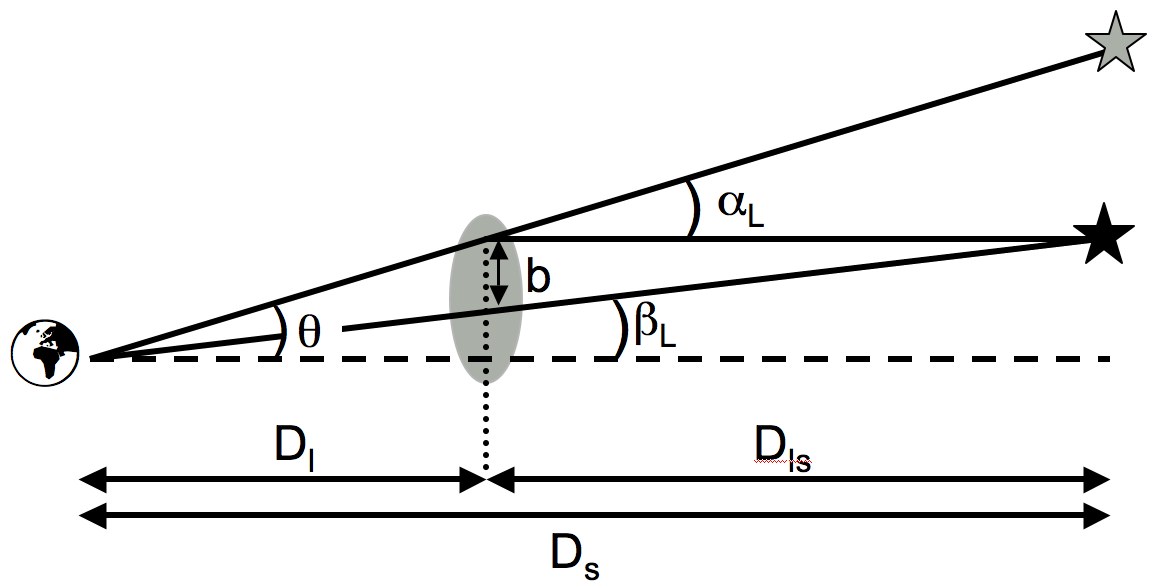
\includegraphics[scale=0.4]{plots_intro/LensDiagram.png}
\caption[Gravitational Lensing Diagram]{Diagram showing the geometry of gravitational lensing. Light from the background source is bent by an angle $\hat{\alpha}_{\rm L}$ when it passes near the gravitational lens (gray oval) on its way to the earth. While the actual source (black star) is at an angle $\beta_{\rm L}$ relative to the horizontal, its image (gray star) appears to be at an angle $\theta$. The angular diameter distances to the lens ($D_{\rm l}$), to the source ($D_{\rm s}$) and between the lens and source ($D_{\rm ls}$) are labeled.}
\label{plot:lensing}
\end{center}
\end{figure}

The fact that gravitational lensing directly probes the underlying density field along the line of sight is what makes the technique extremely valuable. All other methods for probing the matter distribution of the universe do not probe the mass itself (which is mostly dark matter), but rather the baryonic component of the mass -- stars, and interstellar gas and dust. While we expect the baryons to trace the underlying density of dark matter, there are many complicating factors (see \autoref{sec:Clusters}) that render the analogy lacking. Additionally, other means of measuring masses (such as using radial velocities) rely on assumptions about the virial equilibrium of a system which may not be satisfied.

Gravitational lensing is broadly divided into several branches depending upon the strength of the lensing effect. Strong lensing refers to the rarest and most obvious distortions, leading to images of giant arcs, Einstein rings, and multiple images of the same source. Strong lensing features are generally apparent to the eye (see \autoref{plot:abellcluster} for an example), whereas weak lensing and microlensing are not. The first observation of gravitational lensing producing multiple images was made by \citet{Walsh79} using a lensed quasar. The first gravitationally lensed arcs were discovered nearly a decade later by \citet{Lynds86} and \citet{Soucail87,Soucail88}. Currently, over one hundred strong gravitational lenses are known \citep{Browne03,Bolton08}. Strong lensing is very useful for accurately probing the dark matter halo mass profiles of galaxies and clusters of galaxies, often yielding detailed information on lens concentration \citep{Auger10} and substructure \citep{Mao98,Dalal02}. 

\begin{figure}
\begin{center}
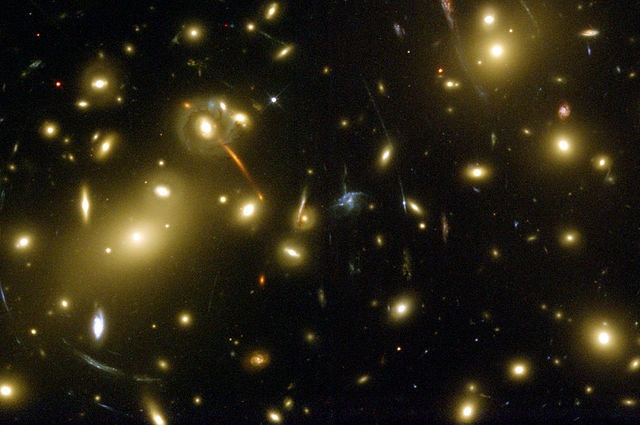
\includegraphics[scale=1.5]{plots_intro/Abell2218_Med.jpg}
\caption[Strong Lensing Image]{Abell 2218, a galaxy cluster at $z \sim 0.18$, yields a magnificent example of strong gravitational lensing. Many large arcs, which are highly distorted images of background galaxies, are easily visible in this image [Source: NASA].}
\label{plot:abellcluster}
\end{center}
\end{figure}

Weak lensing, just as the name implies, leads to much less significant distortions. The hallmark of weak lensing is that it is a statistical effect, only measurable using ensembles of many background sources and foreground lenses. Unlike the rarity of a strong lensing event, however, weak lensing is everywhere. Essentially all light rays are distorted at least a bit while traveling to us through the inhomogeneous gravitational fields of the universe. Weak lensing itself, and different approaches to measuring it, will be discussed in much more detail in \autoref{sec:Shear} and \autoref{sec:Mag} below. 

Finally, microlensing is the even weaker signature of gravitational lensing, wherein stars are lensed by low mass compact objects like black holes, brown dwarfs, and planets. Probably the most important use of microlensing has been the search for a significant \acf{MACHO} population in the Milky Way. \ac{MACHO}s were once considered a serious dark matter candidate until various microlensing experiments demonstrated that the mass density of \ac{MACHO}s was strongly insufficient to explain the missing mass in our galaxy \citep{Paczynski96,Wyrzykowski11,Sumi13}.

%%%%

\subsection{Weak Lensing Shear}
\label{sec:Shear}

Weak lensing shear is the component of weak lensing that deals with shape distortion of galaxy images. If all galaxies were intrinsically circular, or of known shape, then each individual background source would provide information on the gravitational field through which its light had propagated. Instead, however, galaxies take on a variety of shapes and orientations, and their unlensed representations are impossible to know. In order to proceed, weak lensing astronomers make two critical assumptions: (1) galaxy shapes can be approximated as elliptical, and (2) the orientation of these ellipses are random in the absence of gravitational lensing \citep{BS01}. The second point follows from the isotropy of the universe. Though only a few percent effect, characterization of any intrinsic alignments is an active area of research \citep[see e.g.][]{Hirata04,Heymans13}.

As illustrated in \autoref{plot:lensing}, the lens equation is given by 
\begin{equation}
\bm{\beta}_{\rm L} = \bm{\theta} - \bm{\alpha}_{\rm L},
\end{equation}
where we now use bold face to indicate angular positions with two components on the sky. The reduced deflection angle $\bm{\alpha}_{\rm L}$ is related to the deflection angle of \autoref{eqn:deflection} by $\bm{\alpha}_{\rm L} = (D_{\rm ls}/D_{\rm s})\bm{\hat{\alpha}}_{\rm L}$. The reduced deflection angle $\bm{\alpha}_{\rm L}$ can be expressed as the gradient of the lensing (or deflection) potential $\bm{\alpha}_{\rm L} = \nabla \psi$. The lensing potential $\psi(\bm{\theta})$ is the two-dimensional analogue to the Newtonian gravitational potential $\Phi$, and is given by \citep{NarayanBartelmann96}:
\begin{equation}
\psi(\bm{\theta}) = \frac{2}{c^2}\frac{D_{\rm ls}}{D_{\rm l} D_{\rm s}} \int \Phi(D_{\rm l} \bm{\theta},z){\rm d}z = \frac{1}{\pi} \int_{\mathbb{R}^2} \kappa(\bm{\theta'}) {\rm ln}|\bm{\theta} - \bm{\theta}'| {\rm d}^2 \theta'.
\end{equation}
Here $\kappa$ is known as the convergence, which encapsulates the magnification information to be described in \autoref{sec:Mag} below. Explicitly, the convergence is given by
\begin{equation}
\label{eqn:kappapartials}
\kappa(\bm{\theta}) =\frac{1}{2} \left( \frac{\partial^2 \psi(\bm{\theta})}{\partial\theta_1^2} + \frac{\partial^2 \psi(\bm{\theta})}{\partial\theta_2^2} \right),
\end{equation}
and another useful expression is the ratio
\begin{equation}
\label{eqn:kappa}
\kappa(\bm{\theta}) = \frac{\Sigma(\bm{\theta})}{\Sigma_{\rm crit}}.
\end{equation}
Here $\Sigma(\bm{\theta})$ is the two-dimensional surface mass density (with units of mass per area on the sky), and $\Sigma_{\mathrm{crit}}$ is the critical surface mass density of the lens \citep{Wright00}. The latter demarcates the separation between strong and weak gravitational lenses, depending critically on the geometry of the angular diameter distances between objects, given by
\begin{equation}
\label{eqn:sigcrit}
\Sigma_{\mathrm{crit}} = \frac{c^2}{4 \pi G} \frac{D_{\rm s}}{D_{\rm l} D_{\rm ls}}.
\end{equation}
Strong lenses (i.e. capable of forming multiple images) must have $\Sigma \ge \Sigma_{\mathrm{crit}}$ \citep{Schneider06_IntroGravLensCosmology}.

\begin{figure}
\begin{center}
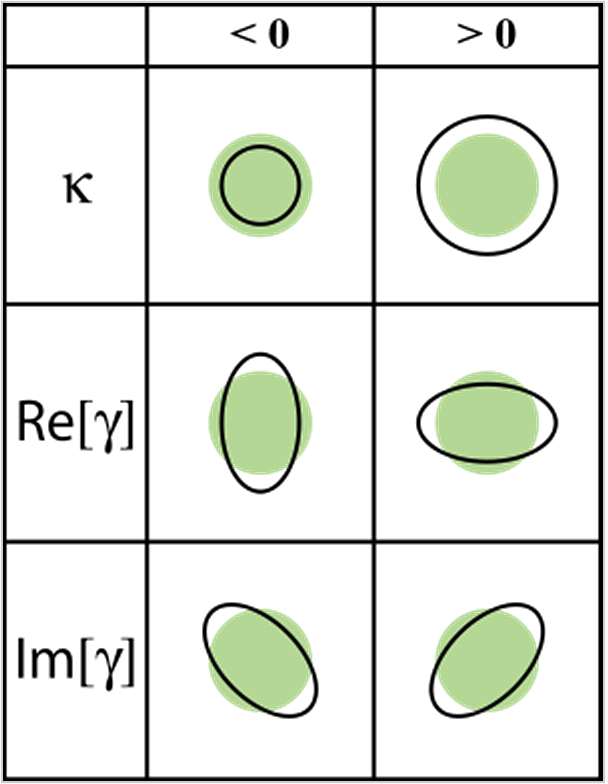
\includegraphics[scale=0.3]{plots_intro/kappa_gamma.png}
\caption[$\kappa$ and $\gamma$ Diagram]{Demonstration of the effect of convergence $\kappa$ and shear $\gamma$ on a circular source. Diagram shows the unlensed source (green circle) and the final lensed image (black outline) for positive and negative values of both $\kappa$ and the real and imaginary components of $\gamma$. [Source: TallJimbo/Wikimedia Commons/CC-BY-SA-3.0].}
\label{plot:kappagamma}
\end{center}
\end{figure}

The transformation of background objects from source (unlensed) to image (lensed) is described by the Jacobian (or amplification) matrix $\cal{A}$ \citep{DodelsonText}: 
\begin{equation}
\label{eqn:A}
{\cal A}(\bm{\theta}) = \frac{\partial \bm{\beta_{\rm L}}}{\partial \bm{\theta}}  = \left( \delta_{ij} - \frac{\partial^2 \psi(\bm{\theta})}{\partial \theta_{i} \partial \theta_j} \right) = \left( \begin{array}{cc}
{1-\kappa-\gamma_1} & {-\gamma_2} \\
{-\gamma_2} & {1-\kappa+\gamma_1} \\
\end{array} \right). 
\end{equation}
The two components of the shear $\gamma (\bm{\theta})$ can be expressed as derivates of the lensing potential:
\begin{equation}
\gamma_1 = \frac{1}{2} \left( \frac{\partial^2 \psi(\bm{\theta})}{\partial\theta_1^2} - \frac{\partial^2 \psi(\bm{\theta})}{\partial\theta_2^2} \right), 
\end{equation}
\begin{equation}
\gamma_2 = \frac{\partial^2 \psi(\bm{\theta})}{\partial\theta_1 \partial\theta_2}.
\end{equation}
The shear is often written as a complex number, $\gamma \equiv \gamma_1 + i\gamma_2 = |\gamma|{\rm e}^{2i\varphi}$. Here $|\gamma|$ and $\varphi$ indicate the amplitude and direction of distortion, respectively, which is unchanged when rotated by 180$^\circ$. An illustration of the meaning of each component of $\gamma$, as well as $\kappa$ is given in \autoref{plot:kappagamma}

We do not observe the true shear, but rather the reduced shear  $g(\bm{\theta}) = \gamma (\bm{\theta}) \left[1-\kappa (\bm{\theta}) \right]^{-1}$. We can thus rewrite the Jacobian matrix as:
\begin{equation}
\label{eqn:Ag}
{\cal A}(\bm{\theta}) = (1-\kappa) \left( \begin{array}{cc}
{1-g_1} & {-g_2} \\
{-g_2} & {1+g_1} \\
\end{array} \right). 
\end{equation}
In the regime of weak lensing, the convergence and shear are small, $\kappa \ll 1$ and $| \gamma| \ll 1$. Therefore it is often safe to assume that $\gamma \approx g$ \citep{Schneider06_WeakGravLens}.

The observed brightness distribution of a galaxy image $I(\bm{\theta})$ is not in general perfectly elliptical, but we can approximate it as an ellipse in the following manner. The center of the brightness distribution of the image is
\begin{equation}
\bm{\bar{\theta}} \equiv \frac{\int {\rm d}^2\theta I(\bm{\theta}) q_I( I(\bm{\theta})) \bm{\theta}}{\int {\rm d}^2\theta I(\bm{\theta}) q_I( I(\bm{\theta}))},
\end{equation}
where $q_I( I(\bm{\theta}))$ is some weight function, and we assume that the galaxy image of interest is isolated on the sky. To describe ellipticity we will be interested in the second brightness moments of the source, contained in the tensor
\begin{equation}
Q_{ij} = \frac{\int {\rm d}^2\theta I(\bm{\theta}) q_I( I(\bm{\theta})) (\theta_i - \bar{\theta_i})(\theta_j - \bar{\theta_j})}{\int {\rm d}^2\theta I(\bm{\theta}) q_I( I(\bm{\theta}))},
\end{equation}
where $i,j \in (1,2)$ \citep{Schneider06_WeakGravLens}. The size $\omega$ of the galaxy image is just a function of the diagonal components of this matrix,
\begin{equation} 
\label{eqn:size}
\omega = (Q_{11}Q_{22} - Q_{12}^2)^{1/2},
\end{equation}
while the shape, or ellipticity, of the image involves the off-diagonal elements:
\begin{equation} 
\chi \equiv \frac{Q_{11} - Q_{22} + 2i Q_{12}}{Q_{11} + Q_{22}} ,
\end{equation}
\begin{equation} 
\epsilon \equiv \frac{Q_{11} - Q_{22} + 2i Q_{12}}{Q_{11} + Q_{22} + 2(Q_{11}Q_{22} - Q_{12}^2)^{1/2}}.
\end{equation}
The complex ellipticity can be characterized by either of $\chi$ or $\epsilon$, which are simply related and interchangeable (in different situations one may be easier to work with) \citep{BS01}. 

In analogy with the image center $\bm{\bar{\theta}}$ and tensor of second brightness moments $Q_{ij}$, one can define the same quantities for the unlensed source center $\bm{\bar{\beta}}$ and tensor of second brightness moments $Q_{ij}^{(s)}$. The relation between the source and image tensors is
\begin{equation}
Q^{(s)} = {\cal A} Q {\cal A}^{\rm T} = {\cal A} Q {\cal A},
\end{equation}
where ${\cal A} \equiv {\cal A}(\bm{\theta})$ is the Jacobian defined in \autoref{eqn:A} and \autoref{eqn:Ag}. The observed source ellipticity $\epsilon$ is related both to the shear caused by weak lensing, and to the intrinsic ellipticity $\epsilon^{(s)}$ of the unlensed background source:
\begin{equation} 
\epsilon^{(s)} = 
    \begin{cases}
        \frac{\epsilon - g}{1-g^*\epsilon}, & \text{for} |g| \le 1 \\
        \frac{1-g\epsilon^*}{\epsilon^* - g^*}, & \text{for} |g| > 1.
    \end{cases}
\end{equation}
If we average over many background sources that are randomly oriented, then the average intrinsic ellipticity $\langle \epsilon^{(s)} \rangle = 0$ and we can apply the weak lensing approximation to conclude that $\gamma \approx g \approx \langle \epsilon \rangle \approx  \langle \chi \rangle /2$ \citep{BS01}. 

In this thesis we are concerned with a particular manifestation of gravitational lensing -- lensing by galaxy clusters. If we consider an circularly symmetric mass density on the sky (an idealized galaxy cluster), then we expect the shear distortion to be oriented tangential to the center of the lens. It is therefore useful in cluster lensing (and also in galaxy-galaxy lensing) to express the shear in terms of tangential and rotated (or cross) components:
\begin{equation}
\gamma_{\rm t} = -{\rm Re}\left[ \gamma {\rm e}^{-2i\phi} \right],  
\end{equation}
\begin{equation}
\gamma_{\rm r} = -{\rm Im}\left[ \gamma {\rm e}^{-2i\phi} \right].
\end{equation}
Here the angle $\phi$ is the azimuthal angle measured about the center of the lens \citep{Schneider06_WeakGravLens}. The rotated shear (which would represent a curl component) should be consistent with zero, and is often used as a check of systematic effects. Even though any single galaxy cluster (or other lens) is likely not perfectly azimuthally symmetric, we expect a stack of many galaxy clusters to yield a symmetric profile on average.

\begin{figure}
\begin{center}
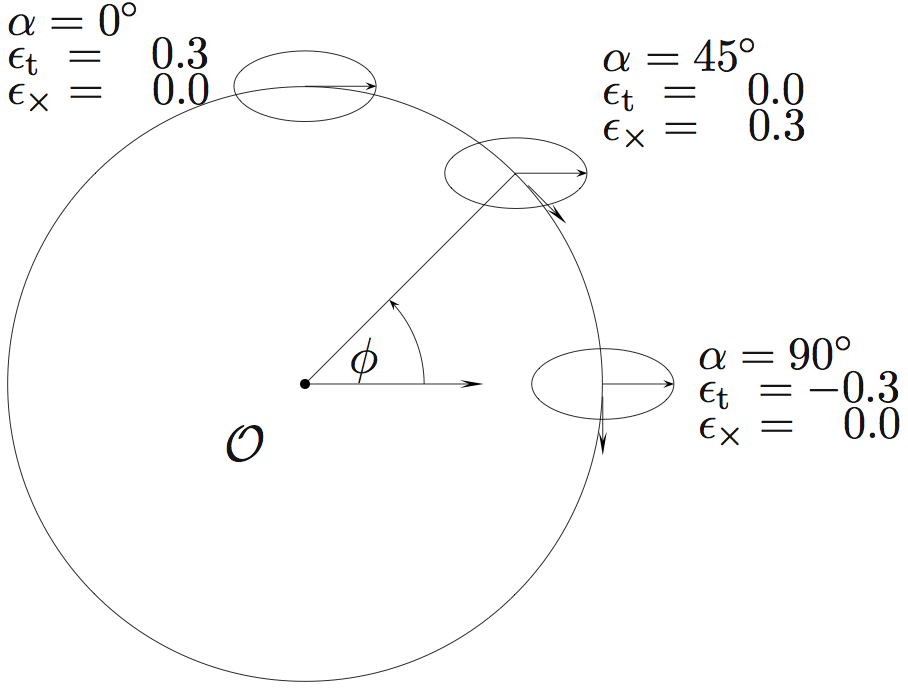
\includegraphics[scale=0.3]{plots_intro/ShearComponents.png}
\caption[Tangential Shear]{Diagram illustrating the components of ellipticity, when decomposed into a tangential and cross component relative to the center of a gravitational lens. As described in the text of \autoref{sec:Shear}, the ellipticities $(\epsilon_{\rm t},\epsilon_{\times})$ are equivalent to the shear $(\gamma_{\rm t},\gamma_{\rm r})$ if they have been averaged over many sources that were randomly oriented in the absence of lensing. The angle $\phi$ measures the azimuthal position of the source about the center of the gravitational lens. [Source: \citet{Schneider06_WeakGravLens}].}
\label{plot:shearcomponents}
\end{center}
\end{figure}

Similar to the surface mass density representation of the convergence (\autoref{eqn:kappa}), we can then relate the tangential shear to the differential surface mass density of the lens:
\begin{equation}
\gamma_{\rm t}(\theta) = \frac{\Delta\Sigma(\theta)}{\Sigma_{\rm crit}},
\end{equation}
where $\theta$ now specifies the radial angle of separation between the lens center and the source image. The differential surface mass density is defined to equal the difference between the average surface mass density interior to $\theta$ and the surface mass density at $\theta$ \citep{Wright00}: 
\begin{equation}
\Delta\Sigma(\theta) \equiv \overline{\Sigma}(< \theta) - \Sigma(\theta).
\end{equation}
Given an expression for the mass density profile of a gravitational lens, and angular diameter distances involved, the expected tangential shear profile can be calculated. Useful models for galaxy cluster masses, and the resulting $\gamma_{\rm t}(\theta)$ and $\Delta\Sigma(\theta)$ profiles, will be given in \autoref{sec:Clusters}.

%%%%

\subsection{Weak Lensing Magnification}
\label{sec:Mag}

Gravitational lensing causes the magnification of background galaxies due to the isotropic focusing of the lensed light rays (whereas shear arises from the anisotropic component). Magnification $\mu(\bm{\theta})$ is related to the determinant of the Jacobian, 
\begin{equation}
\mu  = \frac{1}{{\rm det}{\cal A}} = \frac{1}{(1-\kappa)^2 - |\gamma|^2}.
\end{equation}
In the weak lensing limit ($|\gamma| \ll 1$), the magnification is simply a measure of the convergence of a lensing mass, $\mu \approx 1+2\kappa$, where $\kappa$ is defined in \autoref{eqn:kappapartials} and \autoref{eqn:kappa} \citep{Schneider06_IntroGravLensCosmology}. For the case of circularly symmetric sources we can write $\mu = (\theta/\beta_{\rm L})({\rm d}\theta/{\rm d}\beta_{\rm L})$
\citep{NarayanBartelmann96}. Conceptually, magnification can be understood as the stretching of solid angle on the sky, which causes the amplification of source flux, since lensing conserves surface brightness. This directly leads to a change in source size $\omega = \mu(\bm{\theta}) \omega^{(s)}$, where size is defined in \autoref{eqn:size} \citep{BS01}.

In general, two different approaches can be taken to measure magnification: (1) quantifying sizes of galaxies behind lenses and measuring lensing-induced changes, or (2) detecting the effect on background source number density that ensues as a result of amplification in a flux-limited survey. This thesis focuses on the latter approach. The former method suffers from many of the limitations facing shear analysis, and will be discussed briefly in \autoref{sec:VS} below. 

\begin{figure}
\begin{center}
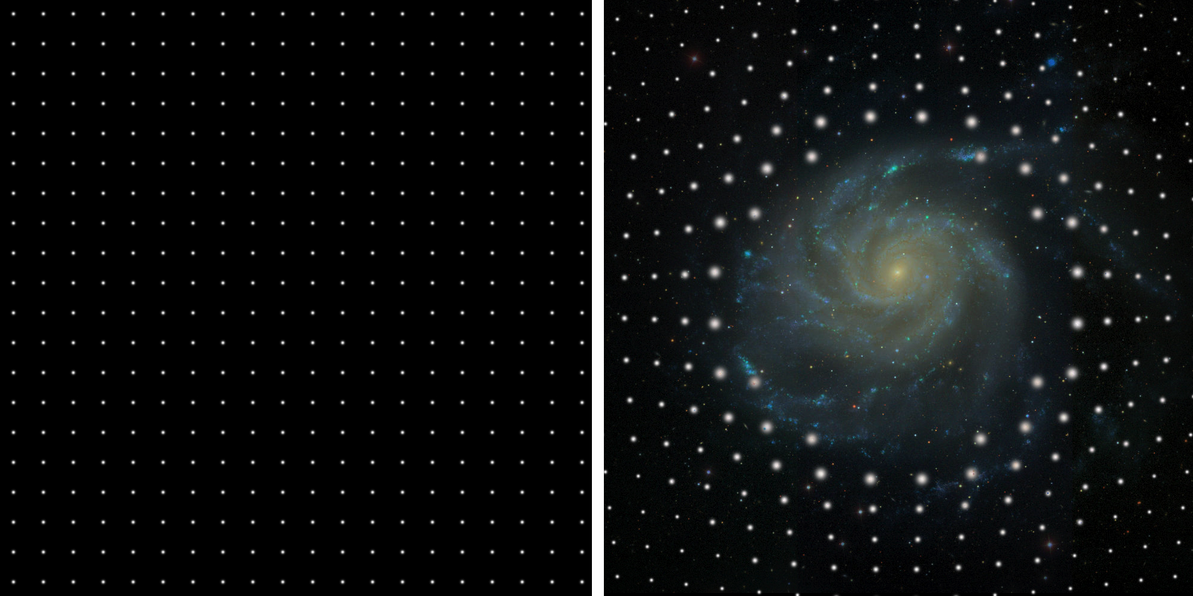
\includegraphics[scale=0.4]{plots_intro/Magnification.png}
\caption[Magnification Illustration]{Highly exaggerated illustration of the two effects of magnification (dilution and amplification) by a massive foreground galaxy. The left panel shows an idealized set of unlensed sources, the right panel shows the effect of gravitational lensing. Dilution refers to the stretching of solid angle on the sky, which reduces background source number density. Since lensing conserves surface brightness, a consequence is that source flux is amplified. [Source: Joerg Colberg, Ryan Scranton, Robert Lupton, \ac{SDSS}].}
\label{plot:magnification}
\end{center}
\end{figure}

Define $n_0(f,z){\rm d}f{\rm d}z$ to be the intrinsic (unlensed) number of galaxies per solid angle within ${\rm d}f$ of flux $f$ and ${\rm d}z$ of redshift $z$. The cumulative lensed number density detectable (i.e. brighter than $f$) in an astronomical survey will then be:
\begin{equation}
n(>f,\bm{\theta},z) = \frac{1}{\mu(\bm{\theta},z)} n_0\left(\frac{>f}{\mu(\bm{\theta},z)},z\right).
\end{equation}
In this equation we can see that magnification affects the source number densities in two ways. The prefactor $1/\mu$ represents the stretching of apparent solid angle, and decreases the number density on the sky. Meanwhile, the denominator in the argument of $n_0$ implies that sources will be detectable to a fainter intrinsic magnitude, effectively increasing the observed source number density if there exist sources fainter than the detection limit of the survey \citep{Schneider06_WeakGravLens}. An illustration of the two effects of magnification is given in \autoref{plot:magnification}.

Since magnification affects the background source number densities in these two opposing ways, we require knowledge of the intrinsic source number densities as a function of brightness, in order to predict or interpret our magnification observations. Typically, astronomical sources such as galaxies contain relatively few very bright members and are much more numerous towards the faint end. If we approximate the slope of the number density in a narrow flux bin as a power law $n_0(f) \propto f^{-\alpha}$, then we have
\begin{equation}
\frac{n(>f)}{n_0(>f)} = \mu^{\alpha-1}.
\end{equation}

Unfortunately, instead of using flux, astronomers frequently characterize source brightness using the ancient-Greek-inspired system of magnitudes. The apparent (observed) magnitude of an object with flux $f$ is
\begin{equation}
m \equiv -2.5 {\rm log}_{10}(f/f_{\rm x}),
\end{equation}
where $f_{\rm x} = 2.53 \times 10^{-8} \ {\rm W}/{\rm m}^2$ is a reference flux. Bright sources have smaller apparent magnitudes. Absolute magnitude $M$ can be defined similarly, but relative to a reference luminosity. Its relation to apparent magnitude can be expressed as $M=m-5{\rm log}_{10}(d_L/10{\rm pc})$, where $d_L$ is the luminosity distance in \autoref{eqn:dL} \citep{RydenText}. In terms of apparent magnitudes we can relate the lensed and intrinsic number densities using the equation
\begin{equation}
\label{eqn:nofm}
n(m,z){\rm d}m = \mu^{\alpha -1} n_0(m,z){\rm d}m,
\end{equation}
where we now define $\alpha$ explicitly according to
\begin{equation}
\alpha \equiv \alpha(m,z) = 2.5 \frac{\mathrm d}{\mathrm d \it m} \log n_0(m,z).
\label{alpha}
\end{equation}
The form of \autoref{eqn:nofm} was first demonstrated by \citet{Narayan89}, who applied it to lensed quasar number densities, but it can be generalized to any galaxy type as long as one has a means of obtaining the slope of the number counts $\alpha$.

Returning to the question of whether gravitational lensing magnification will cause an increase or decrease in observed number densities of background sources, we find that the answer depends precisely on the value of $\alpha$. Sources for which $\alpha -1 > 0$ will appear to be correlated on the sky with a lens position, while sources with $\alpha -1 < 0$ will be anti-correlated, as a dearth of objects will be observed in the vicinity of a lens.  The number density of galaxies for which the intrinsic number count slope gives $\alpha -1 \approx 0$ will essentially be unaffected by lensing magnification, as the dilution and amplification effects will cancel, and no correlation signal will be observed for these objects \citep{Scranton05}. The brightest sources, which usually have steep number counts, will exhibit an {\it increase} in number density when lensed, as the amplification allows more objects to be detected, while the number density of the faintest sources, having relatively shallow number counts, will {\it decrease} \citep{Narayan89}.

Lensing magnification has had an interesting history. During the 1970s and '80s several studies showed that bright quasars were correlated on the sky with foreground galaxies \citep{SeldnerPeebles79,Arp81,Webster88,Narayan89}. The reason for this association was hotly debated, with some astronomers even arguing for physical associations of the objects \citep{Arp87}. The proponents of the lensing interpretation were frequently obtaining results discrepant with eachothers' as well as with the expected lensing signal strength \citep[see e.g.][]{Schneider92} through the end of the 20$^{\rm th}$ century. The first convincing magnification detection was made by \citet{Scranton05}, using 200,000 quasars lensed by 13 million galaxies in the \acf{SDSS}.

Quasars are appealing background sources for magnification studies for two reasons. First of all, their high redshifts ensure that they are well separated from the foreground lenses, which is important so that physical associations due to gravitational attraction do not contaminate the lensing signal. Secondly, their steep number counts yield high values for the slope $\alpha(m,z)$ which leads to strong positive correlations with the lenses. More recently, \acf{LBG} sources have also been used successfully in magnification studies by \citet{Hildebrandt09b},\citet{Morrison12}, and \citet{Hildebrandt13} and by the author of this thesis in \citet{Ford12} and \citet{Ford14} (see \autoref{ch2}and \autoref{ch3}). These galaxies tend to also have high $\alpha(m,z)$ values, but more care must be taken to ensure redshift separation from the lenses involved.

\subsection{Magnification vs. Shear}
\label{sec:VS}

The shear approach to weak lensing has dominated the field for the last several decades. Early work by \citet{Schneider00} showed that shape information had less intrinsic scatter than sizes or number counts, and concluded that very little was gained by including magnification along with shear. A review article by \citet{BS01} compared the signal-to-noise ratios of shear and magnification, finding the shear signal-to-noise to be at least 5 times larger than for magnification. This comparison included several simplifying assumptions, like equal number densities of sources for shear and magnification, and a number count slope of $\alpha=0.5$. However, \ac{LBG}s and quasars can have $\alpha$ values of several, at the bright end of the luminosity function, and magnification with number counts can certainly include many times the number of sources relevant for a shear analysis.

One of the really attractive aspects of magnification is its ability to be applied in regimes where the shear technique starts to fail. Since shear studies require accurate measurements of galaxy shapes, in order for a source to be used at all, it must necessarily be well resolved. Specifically, for lenses at high redshift, and for ground-based surveys facing the extra complication of blurring to to atmospheric seeing, the number density of background sources for which shear can be well-determined is greatly reduced \citep{Waerbeke10}.  This is in stark contrast to magnification studies using source number densities, which have no such requirement for the sources to be resolved at all.  In principle only source magnitudes, redshifts, and positions relative to a lens must be known.  This simple fact makes it possible to extend weak lensing magnification analyses to a much higher redshift than possible for shear, and allows a much higher source density to be included in the analysis \citep{LHJM10}.  

Shear is susceptible to an issue known as the mass sheet degeneracy. This is the fact that, since shear probes differential mass profiles, $\Delta\Sigma(\theta)$, adding a constant mass sheet across an entire lens does not change the measured shear \citep{Falco85,SchneiderSeitz95}. Any weak lensing shear measurement is thus left with some ambiguity (although in practice, if the survey area is large enough, this is usually not a concern). Magnification, which directly probes the surface mass density, $\Sigma(\theta)$, can be used to break this mass sheet degeneracy \citep{Broadhurst95}. The combination of shear and magnification, in order to circumvent this degeneracy has been demonstrated in a series of cluster analyses by \citet{Umetsu11,Umetsu13,Umetsu14}.

Some progress has been made in terms of measuring magnification using source size information \citep{Huff14,Schmidt12}. Unfortunately, the approach of measuring size magnification suffers from many of same limitations as the shear technique, since it also requires quantifying the spatial extent of sources which must necessarily be well resolved. Although back-of-the-envelope calculations by \citet{BS01} showed a larger signal-to-noise ratio for size than for number density magnification, \citet{Schneider06_WeakGravLens} explains how the Point Spread Function circularizes the sources, and that seeing-convolved image sizes are even more difficult to measure than shapes. A related alternative approach to measuring magnification by using the modified redshift distributions of lensed background sources was originally proposed by \citet{Broadhurst95}, and recently demonstrated on observational data by \citet{Coupon13}.

Because the constraint on source resolution is considerably relaxed, ground-based observations can be incorporated to a greater degree with magnification (using number counts) than for shear (or size magnification), as we are not concerned with correcting for the smearing of the image due to the atmospheric Point Spread Function. From the financial perspective, these types of magnification studies are therefore extremely cheap to carry out, since the excellent resolution of space-based telescopes is not required \citep{Hildebrandt09b}. 

The bottom line regarding magnification is that it provides gravitational lensing information that is independent of, and complementary to, the information obtained from a weak lensing shear analysis. Since magnification with source number densities (which is the approach taken in \autoref{ch2} and \autoref{ch3} of this thesis) essentially imposes no additional constraints on a weak lensing shear survey, the ability to perform a magnification analysis comes along for free. Any costless source of cosmological information ought to be investigated and exploited in full. See \citet{Waerbeke10}, \citet{RozoSchmidt10}, and \citet{Umetsu11}, for more detailed discussions of the benefits of combining magnification with shear in gravitational lensing studies.


%%%%%%%%%%%%%%%%%%%%%%%%%%%%%%%%%%%%%%%%%%%%%%%%%%%%%%%%%%%%%%%%%%%%%
\section{Galaxy Clusters}
\label{sec:Clusters}

Clusters of galaxies represent the largest and most massive gravitationally-bound systems to have formed thus far in our universe. They range from associations of only a few nearby galaxies, called groups, all the way up to very rich clusters containing many thousands of members. The distinction between groups and clusters is not well defined, and this thesis will largely use the word ``clusters'' as a blanket term covering all groupings of galaxies. Clusters themselves are observed to clump together into enormous superclusters.

Galaxies were first recognized to cluster together by Charles Messier in 1784, and then independently by F. Wilhelm Herschel in the early 19$^{\rm th}$ century, long before they were actually recognized as very distant galaxies similar to our own (they were called ``nebulae'') \citep{Biviano00}. The first cluster masses were estimated by \citet{Zwicky33}, but it wasn't until the first comprehensive catalog of over two thousand clusters was produced by \citet{Abell58} that the study of galaxy clusters really began to take off. Today hundreds of thousands of galaxy clusters have been cataloged and studied \citep[see e.g.][]{Wen12}.

Because they harbor the deepest gravitational potentials in the universe, clusters are unique laboratories for studying the highest energy phenomena since the big bang. They can be used a testing grounds for general relativity, and gravitational structure formation. Baryonic processes of the intergalactic medium, high energy plasma physics, and the interplay with member galaxies and galaxy evolution, can all be explored using galaxy clusters \citep{Kravtsov12}. This section will discuss the two key uses for studying galaxy clusters -- to constrain cosmology (\autoref{sec:ClusterCosmo}) and to understand astrophysical processes (\autoref{sec:ClusterAstro}) -- with an attempt to highlight the significant aspects of these areas that are relevant to this thesis.

\subsection{Clusters for Cosmology}
\label{sec:ClusterCosmo}
Clusters of galaxies represent the high-mass end of structure formation in the universe, and the most recent objects to have collapsed gravitationally. Quantifying cluster number density as a function of mass can be a sensitive probe of cosmology. Two cosmological parameters that are of particular importance for the study of galaxy clusters are $\Omega_m$ and $\sigma_8$. The first, already discussed in \autoref{sec:Cosmology}, is the matter content of the universe expressed as a fraction of the total energy density. The second parameter, $\sigma_8$, is known as the normalization of the matter power spectrum. It can also be described as the variance in the mass contained within spheres randomly located throughout the universe, with comoving radius $8 h^{-1}$Mpc (hence the subscript ``8'') \citep{Voit05}.

The fact that our universe even contains galaxies and other structures, means that the universe is not perfectly homogeneous. The canonical description is that, at early times there existed slight perturbations in the density field, which underwent gravitational collapse to eventually form the varied structures we observe today. If the average density was $\langle \rho_m \rangle$, then these density perturbations as a function of position can be written as
\begin{equation}
\delta(x) = \frac{\rho_m(x) - \langle \rho_m \rangle}{\langle \rho_m \rangle}.
\end{equation}
The Fourier components of the density perturbations are $\delta_{\rm k}(k) = \int \delta(x) {\rm e}^{i {\bm k} \cdot {\bm x}}{\rm d}^3x$. 

If we believe that the universe is indeed isotropic, and that these perturbations $\delta(x)$ can be described as a Gaussian random field (the simplest case scenario), then we can fully characterize them using the isotropic power spectrum $P(k) \equiv \langle | \delta_{\rm k} |^2 \rangle$ \citep{Kravtsov12}. The power spectrum is often approximated as a power law $P(k) \propto k^n$, where $n=1$ is the special scale-invariant case proposed around the same time by \citet{Harrison70,PeeblesYu70,Zeldovich72}. Recent measurements by \citet{PlanckXVI} have shown that $n \approx 0.96$.

Defining a spherical window function $W(r)$, and its Fourier transform $W_k$, we can write the variance on mass scale $M$ as 
\begin{equation}
\sigma^2 \equiv \left\langle \left| \frac{\delta M}{M} \right|^2 \right\rangle = \frac{1}{(2\pi)^3} \int P(k) |W_k|^2 {\rm d}^3k.
\end{equation}
Thus $\sigma_8$ is simply a special case of the square root of the above expression, wherein a top hat window function of radius $8 h^{-1}$Mpc is used.\footnote{The top hat window function is constant inside the $8 h^{-1}$Mpc radius, zero outside of it, and is normalized so it integrates to one.} This particular radius is historical in nature, simply chosen because $\delta M/M \sim 1$ in spheres of this volume, but it remains widely used in the cosmological literature today \citep{Voit05}. Better constraints now give $\sigma_8 \approx 0.83$ \citep{PlanckXVI}.

At first, when the density constrast was small $\delta(x) \ll 1$, the perturbations simply expanded along with the universe. The modes grew independently, according to the linear growth function \citep{Voit05}:
\begin{equation}
D(a) \propto \frac{\delta \rho}{\rho} \propto \frac{\dot{a}}{a} \int_0^a \frac{{\rm d}a}{\dot{a}^3}.
\end{equation}
Later, as they entered each other's horizon, the overdense regions grew by attracting surrounding matter. Once they reach a critical density contrast $\delta_c$, they collapsed gravitationally and decoupled from the global expansion \citep{Schneider06_IntroGravLensCosmology}. Smaller overdensities merged together to form larger structures, in what is known as hierarchical structure formation. A full mathematical description of the growth of structure is beyond the scope of this introduction,  and the reader is referred to important early papers \citep[e.g.][]{PS74,GottRees75} or more recent excellent reviews on the subject \citep[e.g.][]{Voit05,Schneider06_IntroGravLensCosmology,Kravtsov12}. 

A common approach to extracting cosmological information from galaxy clusters involves measuring the cumulative number density (comoving) of clusters above some mass threshold.  This important quantity $n_M (M,z)$ is known as the cluster mass function. In the original formalism of \citet{PS74} the cluster mass function is given by
\begin{equation}
n_M (M,z) = \frac{\Omega_m \rho_{\rm crit}(z=0)}{M} {\rm erfc}\left[ \frac{\delta_c}{\sqrt{2}\sigma(M,z)} \right].
\end{equation}
Improvements have been made on the Press-Schechter formalism, most notably by \citet{Sheth99} and \citet{Jenkins01}, generalizing to ellipsoidal perturbations and improving parameterizations based on cluster simulations. The cluster mass function $n_M$ depends very specifically on the meaning of the mass of a cluster. A common choice, which will be used throughout this thesis, is the mass parameter $M_{200}$. This is the total mass interior to a radius $R_{200}$, within which the average density is 200 times the critical energy density of the universe, $\langle \rho (r<R_{200}) \rangle = 200 \rho_{\rm crit}(z)$.

There are several difficulties in connecting galaxy cluster observations to theories of structure formation in cosmology. Clusters evolve over time, but we cannot observe the collapse of an individual halo because of the time scales involved. Instead we must make inferences by observing ensembles of clusters at different redshifts. Other issues are the observational difficulties associated with compiling pure and complete samples of galaxy clusters, using techniques that nearly always probe some visible tracer of the cluster dark matter halo. Finally, it is very difficult to accurately know the true mass $M$ that appears in the cluster mass function. Gravitational lensing is the most promising method for obtaining accurate cluster masses, and the work in this thesis is aimed at improving these estimates further, especially for higher redshift clusters. Future experiments may build upon this work to use galaxy clusters to improve constraints on cosmology.

\textcolor{red}{Include power spectrum visualization (pg 81 Schneider hardcopy)?}

\subsection{Clusters for Astrophysics}
\label{sec:ClusterAstro}

Other stuff... \citep{Voit05} Be sure to include NFW profiles and $\Delta\Sigma$ profiles for clusters, as claimed at end of shear section.

\textcolor{red}{\begin{itemize}\item cluster intro pg 30+ Schneider ecopy \item NFW on pg 76, of Schneider hardcopy \item halo abundance, power spectrum, pg 67+/- Schneider hardcopy \item good power spectrum visualization pg 81 Schneider hardcopy \end{itemize}}


%%%%%%%%%%%%%%%%%%%%%%%%%%%%%%%%%%%%%%%%%%%%%%%%%%%%%%%%%%%%%%%%%%%%%%
\section{Impact of this Thesis}
\label{sec:Impact}

This work contained in this thesis has pushed the boundaries of what knowledge can be extracted from weak lensing surveys. By including intrinsically smaller and fainter background sources, which cannot be used in conventional weak lensing studies, we pave the way for a more optimal use of survey data. These gravitationally-lensed sources, which are too small for reliable shape or size measurements, can still be included in a lensing analysis by using the flux magnification formalism described in \autoref{sec:Mag}. The author of this thesis has proven the utility of measuring magnification, through several key publications which appear as chapters in this work, and carried out thorough studies of the systematic effects which provide limitations. 

Prior to this thesis research, weak lensing was dominated by the shear method. This was originally motivated by some early work showing that the signal-to-noise for shear was several times larger than for magnification \citep{Schneider00}. While it is true that, for a fixed sample of galaxies, there is less scatter in galaxy shapes than in galaxy positions, the latter is far easier to measure. This simple fact has motivated the research herein. As lensing studies push to higher redshift, and increasingly rely on blurry ground-based data, we have elevated confidence in our measurements of source positions over difficult shape determinations. 

When this thesis work began, only a handful of magnification studies had been completed. The first ground-breaking theoretical formulation of how number densities of sources could be used to measure masses of clusters was laid out in 1995 by \citet{Broadhurst95}, but it took another 20 years before the first convincing observational detection was made \citep{Scranton05}. Following this significant $8\sigma$ detection of galaxy-magnified quasars in the \ac{SDSS}, several studies followed, achieving magnification detections for lensing of normal galaxies \citep{Hildebrandt09b}, and of blue galaxies behind strong lensing clusters \citep{Umetsu11}. These studies all stopped short of deriving scientifically useful results from the magnification measurements -- they either represented proof-of-concept studies for a new technique, or they demonstrated consistency with a lensing interpretation of the signal.

The work in this thesis made major steps forward in the area of lensing magnification. The author performed the first-ever measurement of magnification by stacked galaxy groups in 2012 (See \autoref{ch2}). This particular work was also the first time that shear and magnification mass estimates and signal-to-noise had been compared \citep{Ford12}. Following this influential work in the \acf{COSMOS} survey, the thesis author transitioned focus to the much larger astronomical survey known as the \acf{CFHTLenS}. 

Two important studies resulted from magnification analyses of the \ac{CFHTLenS} for this thesis (See \autoref{ch3} and \autoref{ch4}). First of all, the most significant magnification detection thus far (at $9.7\sigma$) was published in \citet{Ford14}. More importantly, however, that work moved beyond simple magnification-detection to actual science. The thesis author measured masses of stacked galaxy clusters binned as a function of different attributes (redshift and richness), and the dependence of a magnification signal on these parameters was seen for the first time. A mass-richness scaling relation was determined solely from the magnification results, which is a useful tool for making cosmological inferences from optical cluster surveys, as discussed in \autoref{sec:Clusters}. 

This work contained the important inclusion of a means of accounting for one of the dominant systematic effects for magnification, the contamination of the background sources with low-redshift objects. The formalism was extended from earlier work by \citet{Hildebrandt13}, but allowing for different contamination fractions and models for the halo occupation distribution of the galaxy contaminants. This was the first time that galaxy cluster lenses could be used for magnification in a redshift range where there was known source contamination. Prior to this work, the redshift ranges of overlap had to be avoided because the physically-induced cross-correlations of lens and source objects overwhelmed, and could not be separated from, the magnification signal.

Arguably the most important magnification result in all the literature to date is contained in \autoref{ch4} of this thesis. After the semi-blind magnification analysis of \citet{Ford14}, \citet{Ford15} followed suit with an identical treatment of the same cluster sample, but this time using the weak lensing shear approach. This study contained a detailed comparison between cluster masses measured with the two independent techniques, as a function of different cluster attributes, and contained valuable insights regarding systematic effects that are still important to resolve for magnification. Moving forward, this work frames the case for including magnification, and also pin-points some important issues that must be addressed in future work (see \autoref{ch:conc}).

%%%%%%%%%%%%%%%%%%%%%%%%%%%%%%%%%%%%%%%%%%%%%%%%%%%%%%%%%%%%%%%%%%%%%%
\section{Thesis Overview}
\label{sec:Overview}

The body of this thesis is composed of three published studies that develop the weak gravitational lensing magnification technique, particularly for the study of galaxy clusters, and compare with results using the complementary and much more ubiquitous weak lensing shear approach:
\begin{itemize}
\item \autoref{ch2} contains the first magnification study of galaxy groups and first comparison with shear for stacked lens samples. The data are X-ray selected groups, and high-redshift \ac{LBG}s in the \ac{COSMOS} field.
\item \autoref{ch3} represents the highest-significance magnification detection, and the first magnification study that could be binned as a function of cluster parameters. The data are optically-selected galaxy clusters and high-redshift \ac{LBG}s in the \ac{CFHTLenS} field.
\item \autoref{ch4} is the follow-up shear analysis of the same cluster sample presented in the previous chapter, using the \ac{CFHTLenS} shear catalog for background source shape measurements.
\end{itemize}
Finally, \autoref{ch:conc} wraps up with conclusions on the topic of cluster studies using both magnification and shear, and briefly outlines future directions for progress within the field.

%%%%%%%%%%%%%%%%%%%%%%%%%%%%%%%%%%%%%%%%%%%%%%%%%%%%%%%%%%%%%%%%%%%%%%
\endinput
Any text after an \endinput is ignored.
You could put scraps here or things in progress.


%    2. Main body
% Generally recommended to put each chapter into a separate file

%% The following is a directive for TeXShop to indicate the main file
%%!TEX root = diss.tex

\chapter{Magnification by Galaxy Group Dark Matter Halos}
\label{ch2}

%\begin{abstract}
We report on the detection of gravitational lensing magnification by a population of low-mass galaxy groups, at a significance level of $4.8 \sigma$.  Using X-ray selected groups in the \acf{COSMOS} 1.64 deg$^2$ field, and high-redshift \ac{LBG}s as sources, we measure a lensing induced angular cross-correlation between the samples.  After satisfying consistency checks that demonstrate we have indeed detected a magnification signal, and are not suffering from contamination by physical overlap of samples, we proceed to implement an optimally-weighted cross-correlation function to further boost the signal-to-noise of the measurement. Interpreting this optimally weighted measurement allows us to study properties of the lensing groups.  We find that the group mass profiles are well fit by the \acf{SIS} model, and we implement a multi-\ac{SIS} fit that recovers a distribution of lens masses consistent with the values that have already been well measured using the weak lensing shear technique.  We argue that future weak lensing studies will need to incorporate magnification along with shear, both to reduce residual systematics and to make full use of all available source information, in an effort to maximize scientific yield of the observations.
%\end{abstract}


\section{Introduction}
Weak gravitational lensing is a unique tool for probing the mass distribution of the universe and for constraining dark matter halo properties of galaxies and clusters.  In contrast to alternative mass estimate methods (employing e.g. X-ray temperatures, radial velocities, or mass-to-light ratios), weak lensing does not rely on any assumptions about virial equilibrium and is sensitive to all mass along the line of sight, making no distinction between luminous and dark matter.  

Over the past decade, an enormous international effort has been invested in improving the reliability of weak lensing analysis \citep{step1, step2, great08, great10}, seeking to remove biases and systematic effects that limit the accuracy of the method.  By far most of the work has been focused on measuring the shear signal, the coherent stretching and distortion of distant galaxy shapes by a foreground lensing mass, but recently the magnification signal has begun to attract attention as well \citep{Scranton05, Hildebrandt09b, Hildebrandt11, LHJM10, Umetsu11}.  

Weak lensing magnification is, to first order, a measure of the convergence of a lensing mass.  It can be detected through the stretching of solid angle on the sky, which leads to the amplification of source flux, since lensing conserves surface brightness (i.e. photons are neither created nor destroyed in purely lensing processes). In general, two different approaches can be taken to measure magnification.  The method we employ here involves observing the effects on source number densities; an interesting alternative method is being explored by \citet{Schmidt12}, which makes use of source size and flux information, and employs the same \ac{COSMOS} X-ray groups used in this study.

Magnification affects the source number densities in two ways, and the one that dominates is determined by the intrinsic magnitude number counts of the sources in question.  Simply put, the brightest sources, which usually have steep number counts, will exhibit an {\it increase} in number density when lensed, as the amplification allows more objects to be detected, while the number density of the faintest sources, having relatively shallow number counts, will {\it decrease} \citep{Narayan89}.

Compared to shear measurements, magnification exhibits a slightly lower signal-to-noise ($S/N$) ratio, the reason it has been largely ignored until recently.  However, what magnification lacks in signal strength, it makes up for in terms of its ability to be applied to lenses at higher redshift and to poorly resolved sources \citep{Waerbeke10}.  Since shear studies require measurements of galaxy shapes, in order for a source to be used it must necessarily be well resolved.  This is in stark contrast to magnification studies using source number densities, which have no such requirement for the sources to be resolved at all!  In principle only source magnitudes, redshifts, and positions relative to a lens must be known.  This simple fact makes it possible to extend weak lensing magnification analyses to a much higher redshift than possible for shear, and allows a much higher source density to be included in the analysis.  See \citet{Waerbeke10}, \citet{RozoSchmidt10}, and \citet{Umetsu11}, for more detailed discussions of the benefits of combining magnification with shear in gravitational lensing studies. 

In Section \ref{theory} we review the equations describing the effects of weak lensing magnification on source number densities.  Section \ref{data} gives the properties of the X-ray groups and \ac{LBG}s that are used in this study.  Then Section \ref{results} describes the steps of our analysis, and results of the \ac{SIS} model fitting.  We summarize the results in Section \ref{summary}, and compare with weak lensing shear measurements that have previously been made on populations of galaxy groups.  We use the WMAP7 $\Lambda$CDM cosmological parameters $H_0 =$ 71 km s$^{-1}$ Mpc$^{-1}$ and $\Omega_{\Lambda} = 0.734$ \citep{WMAP7}, and set $\Omega_{\rm m} = 1 - \Omega_{\Lambda}$.

\section{Theory}
\label{theory}
The amplification matrix $\cal{A}$ maps the image deformation from the source to observer frame, and describes the first order effects of gravitational lensing.  
\begin{equation}
\cal{A} = \left( \begin{array}{cc}
{1-\kappa-\gamma_1} & {-\gamma_2} \\
{-\gamma_2} & {1-\kappa+\gamma_1} \\
\end{array} \right) 
\end{equation}
It is a function of the convergence $\kappa$, and the shear $\gamma$, which define the isotropic and anisotropic focusing of light rays, respectively.  The magnification factor $\mu$ is the inverse determinant of this matrix, so that
\begin{equation}
\mu = \frac{1}{\mathrm{det} \cal{A}} = 
\frac{1}{(1-\kappa)^2 - \left|\gamma\right|^2}
\end{equation}
\citep{BS01}.  

The cumulative number counts of distant {\it unlensed} sources $N_0$ are related to the observed {\it lensed} number counts $N$, up to some flux $f$, by the equation
\begin{equation}
N (>f) = \frac{1}{\mu} N_0 \left( > \frac{f}{\mu} \right).
\end{equation}
Here the two distinct effects of weak lensing magnification, on source number counts, are made explicit.  The prefactor of $1 / \mu$ is the dilution of source density, as the observed solid angle on the sky is stretched by a foreground massive lens.  The modification to the flux $f / \mu$ inside the argument of $N_0$ represents the effect of source amplification by a lens, such that one is able to detect intrinsically fainter objects due to gravitational lensing.

Switching from working in fluxes to magnitudes $m$, the differential number count relationship was demonstrated by \citet{Narayan89} to be
\begin{equation}
n(m){\rm d}m = \mu ^{\alpha -1} n_0 (m){\rm d}m,
\end{equation}
where $\alpha$ is defined according to
\begin{equation}
\alpha \equiv \alpha(m) = 2.5 \frac{\mathrm d}{\mathrm d \it m} \log n_0(m).
\end{equation}
Thus distant source galaxies, lensed by an intervening concentration of mass, may have their observed number counts increased {\it or} decreased depending on the sign of the quantity $\alpha -1$.  Sources for which $\alpha -1 > 0$ will appear to be correlated on the sky with a lens position, while sources with $\alpha -1 < 0$ will be anti-correlated, as a dearth of objects will be observed in the vicinity of a lens.  The number density of galaxies for which the intrinsic number count slope gives $\alpha -1 \approx 0$ will essentially be unaffected by lensing magnification, as the dilution and amplification effects will cancel, and no correlation signal will be observed for these objects \citep{Scranton05}.

\section{Data}
\label{data}
\subsection{Lenses}
The lenses in this study consist of X-ray selected galaxy groups in the \ac{COSMOS} Field.  See \citet{Leauthaud10} for the detailed properties of these groups.  From the full sample of 206 groups investigated in the aforementioned study, we use the shear-calibrated mass estimates to construct the most massive subsample of groups for this magnification study. Here masses are characterized by the parameter $M_{200}$, the total mass interior to a sphere of radius $R_{200}$, within which the average density is 200 times the critical. 

%GROUP MASS HISTOGRAM
\begin{figure*}
\begin{center}
%\vspace{-75pt}
%\vspace{-25pt}
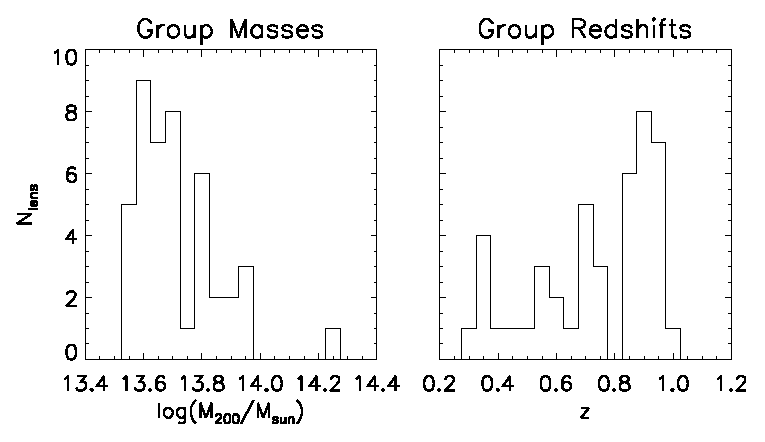
\includegraphics[scale=1.0]{plots_ch2/m200_zphot_histograms_44x.eps}
\caption[Masses and Redshifts of \ac{COSMOS} Groups]{Masses and photometric redshifts of the groups in this study.  We select the most massive groups in our sample, $M_{200} / M_\odot \ge 3.56 \times 10^{13}$. Using only the cleanest groups (characterized by having $\ge$ 4 members, well-defined centroids, and no flags on possible mergers or projection effects), and applying appropriate masking, we are left with a sample of $44$ groups for this lensing magnification analyis.}
\label{hists}
\end{center}
\end{figure*}

Any groups that have less than 4 member galaxies, that appear to be undergoing mergers, that have uncertain centroids, or that raise concerns about projection effects, are excluded from the analysis. These restrictions follow from the group catalog requirement \texttt{FLAG\_INCLUDE=1}, discussed in \citet{George11}. The remaining $44$ most massive groups have shear determined masses in the range $ 3.56 \times 10^{13} \le M_{200} / M_\odot \le 1.70 \times 10^{14} $, and we employ stacking to increase the $S/N$ of the magnification measurement.  The redshift range of the groups is $ 0.32 \le z \le 0.98 $. Figure \ref{hists} displays these lens properties.

Choosing an optimal lens centroid about which to construct angular bins is an area of ongoing research, and common choices include the brightest central galaxy or the X-ray emission peak.  If the location of the dark matter density peak were known {\it a priori}, then it would obviously be the ideal choice, but instead we must rely upon some combination of observables to approximate this position.  In this paper, we define lensing mass centers by the location of the group galaxy with highest stellar mass (MMGG$_\mathrm{scale}$) lying within a distance $ (R_{\rm s} + \sigma_{\rm x}) $ of the X-ray center, where $ R_{\rm s} $ is the group scale radius and $ \sigma_{\rm x} $ is the uncertainty in the X-ray center position \citep{George11}.  In order to be very confident about the locations of group centers, we exclude groups for which this galaxy is not the most massive member of the group.  This choice of centroid has been shown to optimally boost the measured shear signal for this group sample (M. George et al. 2011, in preparation).  

\subsection{Sources}
Background sources are \ac{LBG}s, a type of high-redshift star-forming galaxy that has been used successfully in previous magnification studies \citep[see][]{Hildebrandt09b, Hildebrandt11}. These \ac{LBG}s were selected using the typical three color dropout technique. For the $U$-, $G$-, and $R$-dropouts the selections described in \citet{Hildebrandt09a} were used, however the \ac{COSMOS} Subaru $g^+$ and $r^+$ data were used instead of the \acf{CFHTLS} $g^*$ and $r^*$ data (see \citet{Capak07} for the filter definitions). For the $B$-dropouts the selection from \citet{Ouchi04} was used.  

The appeal of using \ac{LBG}s for magnification is rooted in the fact that their \acf{LF} has been extensively studied and their redshift distributions are fairly narrow and accurate.  After all quality cuts and image masking, we are left with 45,132 \ac{LBG}s in total.  The four distinct sets are comprised of 12,980 $U$-, 22,520 $G$-, 4,870 $B$-, and 4,762 $R$-dropouts, located at redshifts of $\sim$ 3.1, 3.8, 4.0, and 4.8, respectively.

We first test our data selection by cross-correlating the foreground groups with \ac{LBG}s separated into discrete magnitude bins. Here we use the basic \citet{LandySzalay93} estimator, 
\begin{equation}
\mathrm{w}(\theta)=\frac{D_1 D_2 - D_1 R - D_2 R + RR}{RR},
\end{equation}
to simply compute cross-correlations between groups and background sources. $D_1$ and $D_2$ represent the data sets of lenses and sources, and $R$ are the {\it random objects} from a mock catalog we create, containing points uniformly distributed throughout the \ac{COSMOS} survey area. Each product of terms is the number of pairs of those objects found to lie within some angular bin, normalized by the total number of pairs found at all angular separations.  This cross-correlation estimator has been shown to be both robust and unbiased \citep{Kerscher00}.  

In any lensing study, care must be taken to ensure that regions of an image containing artifacts such as saturated pixels, satellite tracks, or other spurious effects, are masked out of the investigation.  We consistently apply the same masks to the group, source, and random catalogs, prior to the correlation analysis. Using a large number (584,586) of objects in this random catalog serves to reduce shot noise.  

We expect that the faintest (brightest) magnitude bins should yield a negative (positive) cross-correlation with the group centers, and this is exactly what we find.  Figure \ref{MagBinned} displays this anticipated result, where we simply use a number count weighted average to combine the signal of the distinct \ac{LBG} samples.  As discussed in \citet{Hildebrandt09b}, this negative correlation is one of the strongest verifications that no redshift overlap exists between lens and source populations, for no viable reason other than lensing magnification can be given for such a signal to exist.  Redshift overlap between samples must be avoided in magnification studies, as positive cross-correlations due to physical clustering would overwhelm any lensing induced signal.

%LBG MAG-BINNED CORR PLOTS
\begin{figure*}
%\centering
\begin{center}
%\vspace{-150pt}
%\vspace{-25pt}
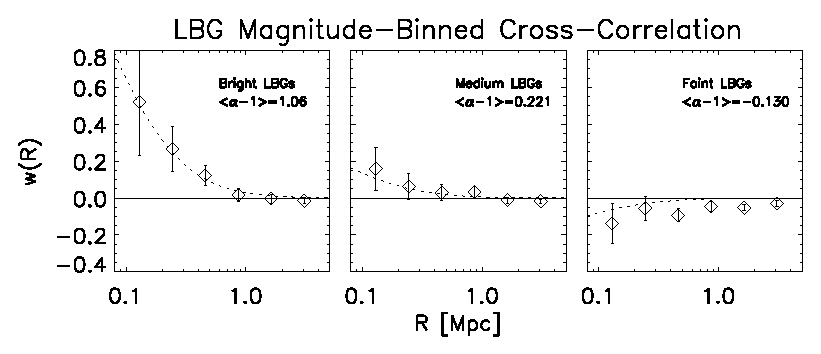
\includegraphics[scale=1.2]{plots_ch2/magbinnedLBGs_multiNFWfit.eps}
\caption[Magnitude-Binned Cross-Correlation]{Angular cross-correlation of the X-ray groups with \ac{LBG}s, the latter separated into 3 magnitude-selected samples.  The Bright sample contains $U$, $G$, $B$, $R$-dropouts in the magnitude ranges $23<r<25$, $23.5<i<25$,  $23.5<i<25$,  $24<z<25.5$, respectively. Similarly, the Medium ranges are $25<r<25.5$, $25<i<26$,  $25<i<26$,  $25.5<z<26$.  The Faint ranges are $r>25.5$, $i>26$,  $i>26$,  $z>26$. These magnitude ranges are selected to contain \ac{LBG}s for which $(\alpha-1)>0$, $\approx 0$, and $<0$.  The measured correlations for each \ac{LBG} sample are simply averaged here (weighting by the number counts) in order to more clearly display this diagnostic check.  The negative correlation observed for the faintest sample is a good indication that no redshift overlap exists between foreground lenses and background sources.}
\label{MagBinned}
\end{center}
\end{figure*}

\section{Analysis and Results}
\label{results}
\subsection{Measuring $\alpha(m)$}
Along with the mass of the lens itself, the slope of the source number counts as a function of magnitude, parameterized by the quantity $\alpha \equiv \alpha(m)$, controls the amplitude and sign of the expected magnification signal.  To interpret the correlations that we measure, and to implement an optimally-weighted procedure, we must determine the value of this quantity for every source galaxy that we intend to use in the measurement.  Fortunately, \ac{LBG}s have been extensively studied and many measurements of their \ac{LF} have been published.  

For the $U$-, $G$-, and $R$-dropouts, we use the recent measurements by \citet{vanderBurg10}. For the $B$-dropouts we use the results of \citet{Sawicki06}. These two sets of measurements both involved fitting a Schechter Function \citep{Schechter76} to their galaxy number counts, and their best fit parameters that we use here, are displayed in Table 1.  The Schechter Function is given by
\begin{equation}
\Phi(M)=0.4\ln(10)\Phi^\ast10^{0.4(\alpha_{\rm LF}+1)(M^\ast-M)} \exp [-10^{0.4(M^\ast-M)}],
\end{equation}
where $\Phi^\ast$, $M^\ast$, and $\alpha_{\rm LF}$ are the normalization, characteristic magnitude, and faint-end slope of the \ac{LF}.  Note that the $\alpha(m)$ which we want to calculate is not the same as the constant parameter $\alpha_{\rm LF}$, but approaches it in the limit of very faint magnitudes.

Solving this equation for $\alpha(m)$, we obtain
\begin{equation}
\alpha(m) = 2.5 \frac{\mathrm d}{\mathrm d \it m} \log n_0(m)= 2.5 \frac{\mathrm d}{\mathrm d \it M} \log \Phi(M) = 10^{0.4(M^\ast-M)}-\alpha_{\rm LF}-1.
\end{equation}
We convert the observed apparent magnitudes $m$ of the \ac{LBG}s to absolute magnitudes $M$ via the relationship $M = m - DM + 2.5 \log (1+z)$, where $DM$ and $z$ are the distance modulus and redshift of the galaxy in question. Since we select apparent magnitudes in the $r$, $i$, and $z$ bands for the $U$-, $G$- and $B$-, and $R$-dropouts, we probe very similar restframe wavelengths and the K-correction between the samples is negligible.  Thus we ignore it here. Using the \ac{LF} parameters in Table \ref{LFtable}, combined with the conversion to absolute magnitudes, we then obtain a robust measure of $\alpha(m)$ for every \ac{LBG} in the sample. 

\subsection{Optimally-Weighted Cross-Correlation}
We implement a modified version of the \citet{LandySzalay93} estimator for the angular cross-correlation function, in which pair counts are weighted by their expectations from the differential source number counts as a function of magnitude.  This weighted correlation function has been shown to optimally boost the magnification signal \citep{Menard03}:    
\begin{equation}
\mathrm{w}(\theta)_{\rm optimal}=\frac{S^{\alpha-1} L - S^{\alpha-1} R - \langle \alpha-1 \rangle LR}{RR} + \langle \alpha-1 \rangle .
\end{equation}
Optimal-weighting was first implemented by \citet{Scranton05} and, apart from notation, this equation is identical to the estimator used in \citet{Hildebrandt09b}.  As with the original basic estimator, each term represents the number of pairs of objects found in a given angular $\theta$ bin, normalized by the total number of pairs at all angular separations.  

$S$ stands for the {\it sources}, or background lensed galaxies, $L$ are the {\it lenses}, or X-ray groups, and once again $R$ are the {\it random objects}. The superscript $\alpha-1$ on the $S$ indicates that pair counts involving sources are to be weighted by this factor.  After removing masked objects from the catalogs, and satisfying the above selection criteria, we are left with 45,132 \ac{LBG} sources, $44$ X-ray group lenses, and 584,586 random objects for the analysis.

%LF TABLE
\begin{table}
  \begin{center}
  %\begin{table*}[h!]
    %\vspace{10pt}
   %\caption{Luminosity Function (Schechter) parameters from external LBG measurements. $^a$ LF parameters from \protect \citet{vanderBurg10}. $^b$ LF parameters from \protect \citet{Sawicki06}.}

    %\begin{tabular}{|l||c|c|c|l|}

   \caption[Luminosity Function Parameters]{\ac{LF} (Schechter) parameters from external \ac{LBG} measurements. $^a$ \ac{LF} parameters from \protect \citet{vanderBurg10}. $^b$ \ac{LF} parameters from \protect \citet{Sawicki06}.}
 \label{LFtable}
\resizebox{0.5\columnwidth}{!}{
    \begin{tabular}{lcccl}
      \hline \hline
      \ac{LBG} Sample & $M^*$ & $\alpha_{\rm LF}$ & Number \\ \hline
      U ($z \sim$ 3.1)$^a$ & -20.84 & -1.60 & 12,980 \\
      G ($z \sim$ 3.8)$^a$ & -20.84 & -1.56 & 22,520 \\
      B ($z \sim$ 4.0)$^b$ & -21.00 & -1.26 & 4,870 \\ 
      R ($z \sim$ 4.8)$^a$ & -20.94 & -1.65 & 4,762 \\
      \hline
    \end{tabular}
}
  \end{center}
\end{table}
%\vspace{-35pt}
%$^a$ LF parameters from \citet{vanderBurg10}.
%$^b$ LF parameters from \citet{Sawicki06}.


The brightest source galaxies, which are observationally found to lie in the steepest part of the \ac{LF}, are expected to be positively correlated with the group centers, have the largest value of $\alpha-1$, and so receive a relatively large weight in this correlation study.  In contrast, the faintest background galaxies are expected to be anti-correlated, on average, with the group positions, because the effects of magnification dilution should be greater than the amplification of flux can compensate for, and these galaxies thus receive a negative weight.  Sources for which $\alpha-1 \approx 0$, ought to have the effects of dilution and amplification cancel out overall, and receive very little to no weight in this analysis \citep{Scranton05}. The optimally weighted correlation function is given in Figure \ref{multisis}, and shows the measured radial profile for this stack of massive galaxy groups.

Error bars are $1 \sigma$ uncertainties, obtained by jackknife resampling of the source population.  To do this, we create 30 jackknife samples of data, each with a different $1/30$ of sources removed from it.  Then we measure the optimal correlation function for each, and from these estimate the covariance matrix through
\begin{equation}
C(\theta_1, \theta_2)= \left( \frac{N}{N-1} \right)^2 \times \sum_{j=1}^N [\mathrm{w}_j(\theta_1)-\bar{\mathrm{w}}(\theta_1)] \times [\mathrm{w}_j(\theta_2)-\bar{\mathrm{w}}(\theta_2)],
\end{equation}
where the index $j$ runs over the $N=30$ jackknife measurements.

\subsection{Halo Mass Profiles}
Measuring the magnification-induced effects on source number counts behind massive lenses allows one to estimate properties of the lens, such as the mass profile.  In this paper we use a \ac{SIS} model to find the best fit mass parameter $M_{200}$ for the groups. We choose the \ac{SIS} primarily for its simplicity as a single-parameter model, in order to demonstrate a proof-of-concept for magnification studies.  Although alternative models, e.g. \acf{NFW} \citep{nfw97}, may better represent the true shape of the halo potential, magnification measurements alone cannot distinguish between the profiles for this small sample.

The \ac{SIS} density profile is $\rho(r)=\sigma_{\rm v}^2/(2 \pi G r^2)$, where $G$ is the Gravitational constant and $\sigma_{\rm v}$ is the velocity dispersion of the lens.  The velocity dispersion can be expressed in terms of the mass and critical energy density of the universe at lens redshift $z$:
\begin{equation}
\sigma_{\rm v} =\left[ \frac{\pi}{6}200\rho_{\rm crit}(z)M_{200}^2 G^3 \right]^\frac{1}{6} .
\end{equation}

The magnification of a \ac{SIS} is given by 
\begin{equation}
\mu_{\rm SIS}(\theta)=\frac{\theta}{\theta-\theta_{\rm E}},
\end{equation}
where $\theta_{\rm E}=4\pi(\frac{\sigma_{\rm v}}{c})^2\frac{D_{\rm ls}}{D_{\rm s}}$ is the Einstein radius of the lens, and $D_{\rm ls}$ and $D_{\rm s}$ are angular diameter distances between lens and source, and observer and source, respectively.

To account for the range of lens masses and redshifts, we perform a multi-\ac{SIS} fit similar to \citet{Hildebrandt11}.  The optimally weighted correlation function is related to the magnification constrast, $\delta\mu(\theta) \equiv \mu(\theta) -1$, through
\begin{equation}
\mathrm{w}(a)_{\rm optimal}= \frac{1}{N_{\rm l}}\sum_{i=1}^{N_{\rm l}} \langle (\alpha -1)^2 \rangle_i \delta \mu_{\rm SIS} (z_i, aM_{{\rm shear},i}),
\end{equation}
where $i$ runs over all lenses. We use the minimum-$\chi^2$ method to fit the multi-\ac{SIS} profile to the magnification measurements (see Fig. \ref{multisis}). The $\chi^2/{\rm dof}$ of the multi-\ac{SIS} fit is 2.3 ($\chi^2=11.5$, ${\rm dof}=5$), and is calculated using the unbiased inverse covariance matrix, according to the prescription in \citet{Hartlap07}.

Here the fit parameter $a$ characterizes the scaling relation between the $M_{200}$ previously measured from the shear, and the best fit $M_{200}$ from magnification, so that $a \equiv M_{\rm magnification}/M_{\rm shear}$. This approach allows us to fit for a range of masses, thereby avoiding any biases that would be introduced by simply fitting to a stacked average lens profile.  We obtain a best fit value of $a=1.4 \pm 0.6$, indicating consistency between the shear and magnification mass estimates for this lens sample.

%syntax for different +/-: $a=1.12_{-0.39}^{+0.35}$

%PLOT OF LBG MULTI-SIS FIT
\begin{figure*}
\begin{center}
%NOTE: for Thesis, Latex didn't show this plot when the name contained an extra "."
% example: wopt_nfw_sis_44x_LFam1_aveErr0.7magcut.eps doesn't work!
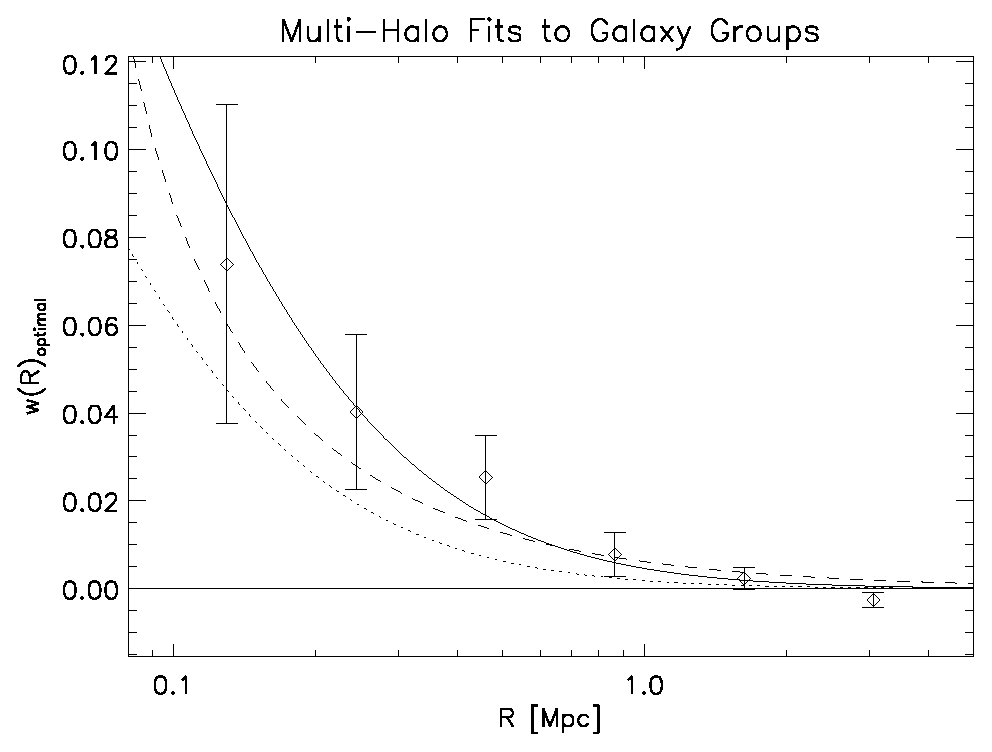
\includegraphics[scale=1.0]{plots_ch2/wopt_nfw_sis_44x_LFam1_aveErr07magcut.eps}
\caption[Optimally-Weighted Cross-Correlation]{Multi-\ac{SIS} fit to the optimally weighted correlation function, using the \ac{LBG} background source sample. The significance of the magnification detection is $4.8 \sigma$.  The dashed line shows the prediction from the shear measured values of $M_{200}$ (A. Leauthaud 2011, private communication), and the solid line is the best fit to the magnification measurement.  We find the best fit relative scaling relation to be $a= M_{\rm magnification}/M_{\rm shear}=1.4 \pm 0.6$, consistent with the shear-measured group masses.  It must be noted that the shear values for $M_{200}$ were calculated assuming an \ac{NFW} profile, but the dashed line plotted here is the resultant \ac{SIS} achieved from applying these masses in an \ac{SIS} context, for comparison.}
\label{multisis}
\end{center}
\end{figure*}

%PLOT OF LBG CORRELATION MATRIX
%\begin{figure*}
%\begin{center}
%\includegraphics[scale=0.5]{CorrMatrix_UGRBall_6R6.pdf}
%\caption{Correlation matrix (normalized covariance matrix) for the optimally weighted correlation measurement using the LBG background sample.}
%\end{center}
%\end{figure*}

\section{Summary and Conclusions}
\label{summary}
We report a $4.8 \sigma$ detection of weak lensing magnification from a population of X-ray selected galaxy groups. This is the first magnification measurement using source number densities successfully performed on low-mass groups. \citet{Schmidt12} has recently explored the magnification of these groups using source sizes and fluxes.  For comparison, the shear detection significance is $11 \sigma$ on the same selection of $44$ groups (A. Leauthaud 2011, private communication).\footnote{The significance quoted for the shear does not take into account the full covariance matrix, as we have done for the magnification measurement.  Therefore this shear significance might be a bit optimistic.}

To improve $S/N$ in this measurement, we stack the lenses, consisting of $44$ massive X-ray detected galaxy groups in the \ac{COSMOS} 1.64 deg$^2$ field.  We measure an optimally-weighted cross-correlation between the X-ray groups and high-redshift \ac{LBG}s, with $1 \sigma$ error bars determined from jackknife resampling of the sources. Performing a multi-\ac{SIS} fit to this optimally-weighted signal yields a measurement of the relative scaling between shear and magnification derived masses. Our magnification measurement yields a mass $M_{\rm magnification}=aM_{\rm shear}$ where the best fit parameter $a=1.4 \pm 0.6$, consistent with the shear mass estimates.

We claim that \ac{LBG}s are a preferred source sample when it comes to performing weak lensing magnification analyses using source number counts.  A few reasons for the superiority of the \ac{LBG} sample include more reliable redshift determinations, as well as greater lensing efficiencies and generally much higher values of the quantity $\alpha-1$.  The single most significant reason to choose \ac{LBG}s for this type of analysis, however, is for the ease of obtaining a reliable measure of $\alpha(m)$.  Previous deep measurements of \ac{LBG} \ac{LF} allow us to perform very simple calculations yielding the optimal weight factor $\alpha-1$.

Although the $S/N$ of shear is superior to magnification in general, the latter probes the surface mass density of the lens directly, while the shear measures the differential mass density.  Thus the combination of these two independent measurements is desirable, and breaks the lens mass-sheet degeneracy. In fact, \citet{RozoSchmidt10} demonstrated that joining magnification into shear analyses, independent of survey details, can improve statistical precision by up to 40-50\%. Magnification using source number densities is also far less sensitive to the effects of atmospheric seeing than either shear or magnification using source sizes.  Both of these methods require quality source images which, for very high-redshift sources, can currently only be obtained from space-based data.

Improving the overall weak lensing derived constraints on cosmological and astrophysical parameters is not the only benefit to incorporating magnification into our analyses, however. Measurements of magnification are sensitive to completely different systematics than shear, and therefore uniquely positioned to help improve calibration of these residual effects on shear measurements.  For example, magnification (using number counts) is not at all sensitive to the possible intrinsic alignment of source galaxies, since it does not use any shape information. Magnification can also be used as a simultaneous probe of intergalactic dust extinction, a small but measurable effect through its wavelength dependence \citep{Menard10}, and as a direct way to measure galaxy bias \citep{Waerbeke10}.

As one proceeds to investigate dark matter structures at increasingly high redshift, it becomes more and more important to include the magnification component of the signal.  This is a direct consequence of the fact that higher redshift lenses necessitate more distant sources, which are in turn much harder to measure shapes for. Proceeding exclusively with shear necessarily means that a high fraction of detected sources are being eliminated from the lensing analysis, and information is therefore being lost, simply because we lack the capabilities to robustly determine their shapes.  With photometric redshifts available, the possibility to do magnification studies on our shear catalogs really comes along free of charge. Upcoming projects will survey the entire extragalactic sky, and the inclusion of magnification will be a necessary component of any robust weak lensing study.
 %COSMOS Magnification
%% The following is a directive for TeXShop to indicate the main file
%%!TEX root = diss.tex

\chapter{Cluster Magnification and the Mass-Richness Relation in CFHTLenS}
\label{ch3}

%\begin{abstract}
Gravitational lensing magnification is measured with a significance of 9.7$\sigma$ on a large sample of galaxy clusters in the Canada-France-Hawaii Telescope Lensing Survey (CFHTLenS). This survey covers $\sim$154 deg$^2$ and contains over 18,000 cluster candidates at redshifts $0.2 \leq z \leq 0.9$, detected using the 3D-Matched Filter cluster-finder of \citet{Milkeraitis10}. We fit composite-NFW models to the ensemble, accounting for cluster miscentering, source-lens redshift overlap, as well as nearby structure (the 2-halo term), and recover mass estimates of the cluster dark matter halos in range of $\sim10^{13} M_\odot$ to $2\times10^{14} M_\odot$. Cluster richness is measured for the entire sample, and we bin the clusters according to both richness and redshift. A mass-richness relation $M_{200} = M_0 (N_{200} / 20)^\beta$ is fit to the measurements. For two different cluster miscentering models we find consistent results for the normalization and slope,  $M_0 = (2.3 \pm 0.2) \times 10^{13} M_\odot$, $\beta = 1.4 \pm 0.1$ and $M_0 = (2.2 \pm 0.2) \times 10^{13} M_\odot$, $\beta = 1.5 \pm 0.1$. We find that accounting for the full redshift distribution of lenses and sources is important, since any overlap can have an impact on mass estimates inferred from flux magnification.
%\end{abstract}


\section{Introduction}
Clusters of galaxies are the most massive gravitationally bound structures in the Universe today. As such they can be useful cosmological probes, as well as laboratories for all kinds of interesting physics including galaxy evolution, star formation rates, and interactions of the intergalactic medium. There are several methods commonly used to estimate cluster masses (e.g., mass-to-light ratios, Xray luminosities, the Sunyaev-Zeldovich effect), but among them gravitational lensing is unique in being sensitive to all mass along the line of sight, irrespective of its type or dynamical state \citep{BS01}.

There are multiple ways to measure the signature of gravitational lensing, and each has its own specific advantages and limitations. Observation of strong lensing arcs and multiple images is extremely useful for studying the innermost regions of clusters, and getting precise mass estimates, but can only be applied to very massive objects which are observationally limited in number. On the other hand, weak lensing shear, which measures slight deformations in background galaxy shapes, can be applied across a much wider range of lens masses. Shear studies have been used with much success to map large scale mass distributions in the nearby universe \citep{Waerbeke13, Massey07}. However, because they rely on precise shape measurements, shear faces the practical limitation of an inability to sufficiently resolve sources for lenses more distant than a redshift of about one \citep{LHJM10}.

A third approach to measuring gravitational lensing is through the magnification of background sources, observable either through source size and flux variations \citep{Schmidt12,Huff14}, or the resultant modification of source number densities \citep{Ford12, Morrison12, Hildebrandt13, Hildebrandt11, Hildebrandt09b, Scranton05}. Magnification has been recently measured using quasar variability as well \citep{Bauer11}. Although relative to the shear, magnification will tend to have a lower signal-to-noise for typical low-redshift lenses, the requirement for source resolution is completely removed. This makes magnification competitive for higher redshift lenses, and especially for ground based surveys where atmospheric seeing has a strong influence on image quality.

In this work we adopt the number density approach, known as flux magnification, using Lyman-break galaxies (LBGs) for the lensed background sources. The observed number density of LBGs is altered by the presence of foreground structure, due to the apparent stretching of sky solid angle, and the consequential amplification of source flux. Because of the variation in slope of the LBG luminosity function, magnification can either increase or decrease the number densities of LBGs, depending on their intrinsic magnitudes. By stacking many clusters we can overcome the predominant source of noise - physical source clustering \citep{Hildebrandt11}. 

In Section \ref{data} we describe the cluster and background galaxy samples. Section \ref{method} lays out the methodology for the measurement and modeling of the magnification signal. We discuss our results in Section \ref{results} and conclude in Section \ref{conc}. Throughout this paper we give all distances in physical units, and use a standard $\Lambda$CDM cosmology with $H_0 =$ 70 km s$^{-1}$ Mpc$^{-1}$, $\Omega_M = 0.3$, and $\Omega_{\Lambda} = 1 - \Omega_M = 0.7$.

%-----------------------------------------

\section{Data}
\label{data}
For the magnification results presented in this paper, we are fortunate to work with a very large sample of galaxy cluster candidates and background galaxies in the Canada-France-Hawaii-Telescope Lensing Survey (CFHTLenS\footnote[1]{www.cfhtlens.org; \\Data products available at http://www.cadc-ccda.hia-iha.nrc-cnrc.gc.ca/\-community/\-CFHTLens/\-query.html}; \citet{Erben13}; \citet{Hildebrandt12}). CFHTLenS is based on the Wide portion of the Canada-France-Hawaii Telescope Legacy Survey, with deep 5 band photometry. The survey is composed of four separate fields, in turn divided into 171 individual pointings, covering a total of 154 deg$^2$.

\subsection{3D-MF Galaxy Clusters}
\label{clusters}
The 3D-Matched-Filter (3D-MF) cluster finding algorithm of \citet{Milkeraitis10}, essentially creates likelihood maps of the sky (in discrete redshift bins) and searches for peaks of significance above the galaxy background. The likelihood is estimated assuming that clusters follow a radial Hubble profile as well as a Schechter luminosity function. A significance peak of \textgreater 3.5$\sigma$ is considered a cluster detection, since this reduces below 1\% the probability of Gaussian random noise fluctuations mimicking a true cluster. The reader is referred to \citet{Milkeraitis10} for the details of the 3D-MF algorithm; here we discuss only the essential points relevant to our purposes. 

The radial component of the 3D-MF likelihood employs a cutoff radius of 1 Mpc, which was chosen to roughly correspond to the radius $r_{200}$ of an $M_{200} \sim 3 \times 10^{13} M_{\odot}$ cluster. \citet{Milkeraitis10} motivates this choice by the desire to optimally search for relatively high mass clusters, but notes that this radius will be less ideal for low mass clusters. One should expect that random galaxy interlopers may contaminate the estimation of significance for likelihood peaks corresponding to lower mass clusters. This may be a key factor in explaining the wide range of cluster significances conferred upon low mass clusters from simulations, while high mass simulated clusters were assigned significances that correlated strongly with mass \citep[see Figure 10 in][]{Milkeraitis10}. Because peak significance may therefore not be an ideal mass proxy to use for the full cluster ensemble, in this work we rely upon a measure of the cluster richness, which is discussed in Section \ref{rich} below. Using cluster richness has the added benefit that the mass-richness relation can be measured and used as a scaling relation.

Using the 3D-MF method, a total of 18,036 galaxy cluster candidates (hereafter clusters) have been detected in CFHTLenS, at a significance of \textgreater 3.5$\sigma$ above the background. In contrast to previous cluster magnification studies, which have been limited by small number statistics, this huge sample of clusters allows us to pursue multiple avenues of investigation. In particular, we bin the clusters according to both richness and redshift, to recover trends in physical characteristics such as the mass-richness relation, and also investigate halo miscentering as a function of these parameters.

\subsubsection{Cluster Centers}
\label{centering}
Due to the nature of the method, the defined centers of the 3D-MF clusters, which are located at peaks in the likelihood map, do not necesssarily coincide with member galaxies. Hence the defined centers are notably different from many other cluster finders, which commonly choose the brightest cluster galaxy (BCG), the peak in X-ray emission, some type of (possibly luminosity-weighted) average of galaxy positions, or a combination of these, as a measure of the center of a dark matter halo.

%PofRcentoff Plot GAUSSIAN MISCENTERING
%\begin{multicols}
\begin{figure}
\begin{center}
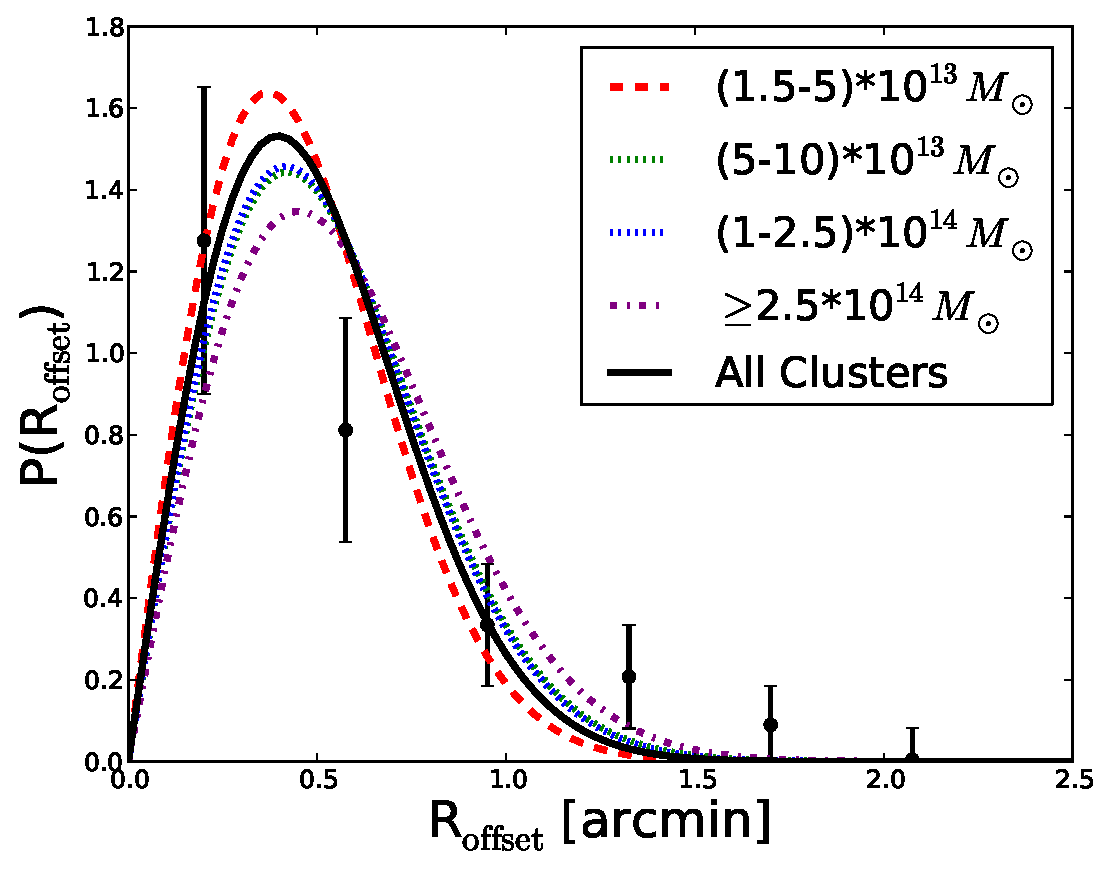
\includegraphics[scale=0.6]{plots_ch3/PofRc_bestfit_python.eps}
\caption[Centroid Offset Model]{Modeled Gaussian distribution of radial offsets between defined 3DMF centers and simulated cluster centers. The black points and solid curve is the combined data and best fit for all CFHTLenS clusters combined. The colored curves show the best fit Gaussians for separate mass bins, and colors match the empirical offsets measured and presented in Figure 13 of \citet{Milkeraitis10}. As each of these colored curve fits is consistent with the solid black curve for the entire combined sample, we choose to use this single Gaussian distribution to model miscentering for all clusters.}
\label{gauss}
\end{center}
\end{figure}
%\end{multicols}

%Sigma_centoff Table GAUSSIAN MISCENTERING
\begin{table}
  \begin{center}
    \caption[Centroid Offset Fit Parameters]{Best Fit Gaussian Distributions for the Cluster Miscentering in Figure \ref{gauss}.}
\resizebox{0.5\columnwidth}{!}{
    \begin{tabular}{llll}
      \hline
      Mass Range [$M_{\odot}$] & Color & Best fit $\sigma_{\mathrm{offset}}$ [arcmin] & $\chi^2_{red}$ \\ \hline
      (1.5-5)$\times10^{13}$ & red    & 0.37$\pm$0.06 & 1.8  \\
      (5-10)$\times10^{13}$  & green  & 0.42$\pm$0.06 & 1.4  \\
      (1-2.5)$\times10^{14}$ & blue   & 0.42$\pm$0.06 & 1.2  \\ 
      $\geq$2.5$\times10^{14}$   & purple & 0.45$\pm$0.06 & 1.4  \\ \hline
      $\geq$1.5$\times10^{13}$  & black  & 0.40$\pm$0.06 & 1.1  \\
      \hline
    \end{tabular}
}
  \end{center}
\end{table}

The choice of cluster center is always ambiguous, both observationally and in simulations. One wants to know the center of the dark matter distribution, as the point around which to measure a radially-dependent signal. Obviously the dark matter cannot be directly seen, so an observable such as galaxies or X-ray emission must be used (see \citet{George12} for an excellent review and analysis of cluster centroiding). The chosen center of the cluster can be wrong for several reasons. The observable chosen (e.g. the BCG) may simply be offset from the true center of the dark matter potential. Misidentification of the BCG can be a significant problem for this particular example as well \citep{Johnston07}. 

Perhaps a more interesting source for miscentering comes from the fact that clusters halos are not perfectly spherical, and exhibit substructure and irregularities caused by their own unique mass assembly histories. Especially for very massive halos, which have formed more recently and in many cases are still undergoing mergers and have yet to virialize, we really should not expect a clear center to exist. Following visual inspection, \citet{Mandelbaum08b} chose to exclude the most massive clusters from their weak lensing analysis for this very reason. Instead of throwing away the highest mass halos in our sample, we include them in this study, but take care to account for possible miscentering effects. 

\citet{Milkeraitis10} tested for centroid offsets in 3D-MF by running the cluster-finder on simulations and comparing detected cluster centers to known centers. The simulations used were the mock catalogs of \citet{KW07}, which were created from a semi-analytic galaxy catalog \citep{DeLucia07} derived from the Millenium Simulation \citep{Springel05}. Figure 13 of that work shows the number of clusters detected as a function of distance from true cluster center. Because 3D-MF was optimized to produce cluster catalogs that are as complete as possible (in contrast to, e.g. \citet{Gillis11}, which is designed to maximize purity), the trade-off is the presence of some contamination with false-detections, especially at the low mass end.

We use the numbers of clusters at each offset, and the contamination from \citet{Milkeraitis10}, to estimate the probability of radial offsets $P(R_{\mathrm{offset}})$. We fit the result for each mass bin with a 2-dimensional Gaussian distribution:
\begin{equation}
P(R_{\mathrm{offset}}) = \frac{R_{\mathrm{offset}}}{\sigma_{\mathrm{offset}}^2} \exp \left[ -\frac{1}{2}\left( \frac{R_{\mathrm{offset}}}{\sigma_{\mathrm{offset}}} \right)^2 \right].
\label{PofRc}
\end{equation}
This resulting curves are presented in Figure \ref{gauss} (colors are selected to match those in Figure 13 of \citet{Milkeraitis10}), and for clarity we only show the data points for the bin that combines all clusters. We find consistent fits for the separate mass bins, which we list in Table 1, and therefore use the combined distribution (black curve) to model the effects of miscentering in our measurements.


\subsubsection{Cluster Richness}
\label{rich}
We define the richness parameter $N_{200}$ in this work to be the number of galaxies within a radius $r_{200}$, and redshift $\Delta z$, of a cluster candidate center (both points discussed below). Member galaxies are also required to be brighter than $i$-band absolute magnitude -19.35. This cut-off is chosen to correspond to the limiting {\it apparent} magnitude of CFHTLenS ($i \sim 24$) at the highest redshift clusters that we probe, $z \sim 1$. So at the expense of removing many galaxies from the richness count, we hope to largely avoid the effect of incompleteness on the number of galaxies per cluster. Then clusters of the same intrinsic richness at high and low redshift should have comparable observed $N_{200}$, within the expected scatter of the mass-richness relation.

For the line-of-sight dimension, we require galaxies to fall within $\Delta z < 0.08(1+z)$ of the cluster redshift. This $\Delta z$ is the 2$\sigma$ scatter of photometric redshifts in the CFHTLenS catalog, chosen so that we reduce the probability of galaxies in a cluster being missed due to errors in their photo-$z$ estimation. Of course this comes at the expense of counting galaxies within a quite broad line-of-sight extent, especially for the higher redshift clusters. This effect should cancel out though, since we also use the same $\Delta z$ range in calculating the galaxy background density, which is subtracted to yield $N_{200}$ as an overdensity count of cluster galaxy members.

%CLUSTER HISTOGRAM (in a single column)
%\begin{multicols}
\begin{figure}
\begin{center}
%\vspace{0.5 cm}
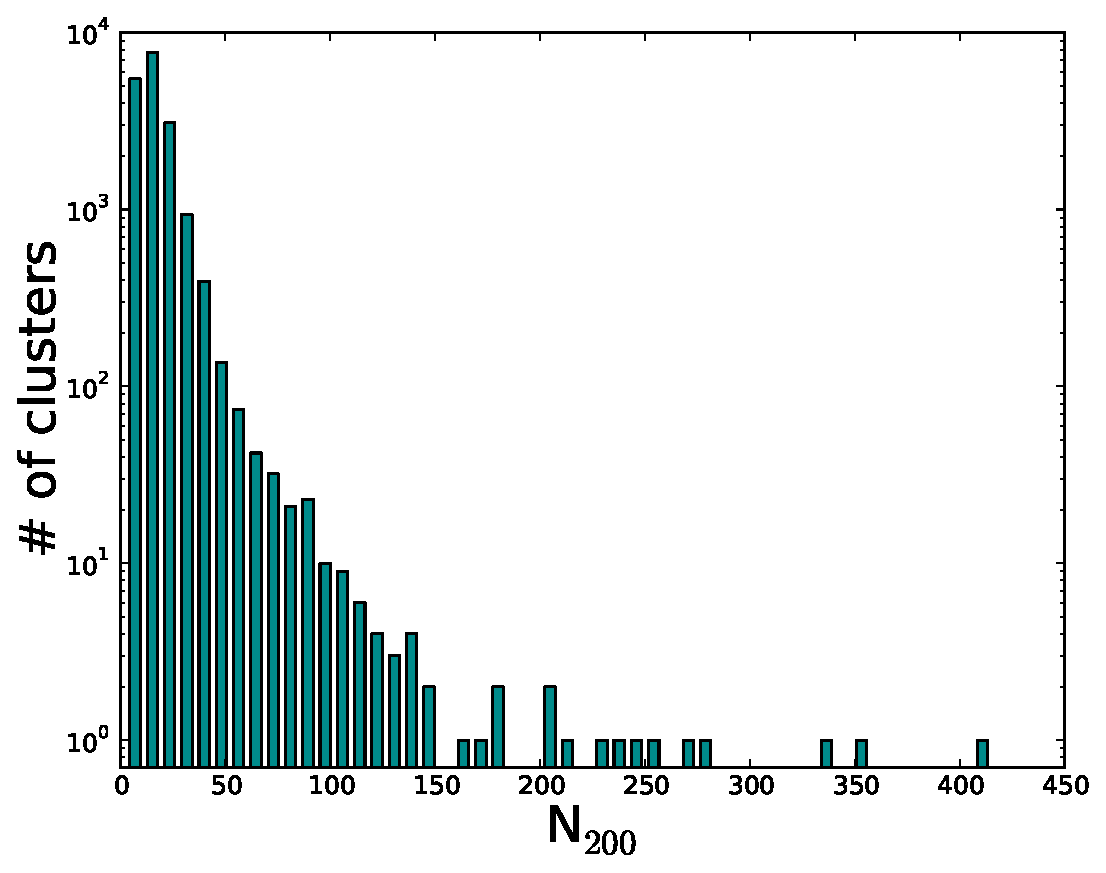
\includegraphics[scale=0.6]{plots_ch3/N200histogram.eps}
\caption[3D-MF Cluster Richness Distribution]{Distribution of richness ($N_{200}$) values for clusters in this study.}
\label{hist}
\end{center}
\end{figure}
%\end{multicols}

In the plane of the sky, galaxies must lie within a projected radius $r_{200}$ of the cluster center (defined above). $r_{200}$ is defined as the radius within which the average density is 200 times the critical energy density of the universe, $\rho_{crit}(z)$, evaluated at the redshift of the cluster. However, since $r_{200}$ itself is unknown, we require some kind of assumption about radius or mass in order to proceded with the galaxy counting. There is no unique way to do this. We begin by making an initial approximation of the masses using a best fit power-law relation between mass and cluster peak significance, for 3D-MF clusters \citep{MMthesis11}:
\begin{equation}
\mathrm{log}(M_{200}) = 0.124 \sigma + \mathrm{log}(10^{14} M_{\odot}) - 1.507.
\end{equation}

As discussed in \ref{clusters}, 3D-MF tests on simulations suggested that peak significance was a good mass proxy for high, but not low, mass clusters. In light of this, we merely employ the above relation as a starting point for calculating the radii from mass,
\begin{equation}
r_{200} = \left[ \frac{3 M_{200}}{4 \pi (200) \rho_{crit}(z)} \right] ^ {1/3}.
\end{equation}
These $r_{200}$ estimates are then used for counting galaxies for cluster richness. Richness $N_{200}$ is the variable of choice used as a mass proxy for binning the magnification measurement. The distribution of these richness values is shown in Fig. 2.

%-----------------------------------------

\subsection{Sources}
We use Lyman-break galaxies (LBGs) as the magnified background sources. LBGs are high-redshift star-forming galaxies \citep{Steidel98}, that have been succesfully employed in past magnification studies \citep[see][]{Hildebrandt09b, Hildebrandt11, Morrison12, Ford12} due to the fact that their redshift distributions and luminosity functions are reasonably well understood. Knowledge of the intrinsic source luminosity function allows for an interpretation of the magnification signal, which depends sensitively on the slope of the number counts as a function of magnitude. In addition, the high-redshift nature of LBGs is important to reduce redshift overlap between lenses and sources. Any source galaxies in the redshift range of the cluster lenses will contaminate the lensing-induced cross-correlation signal, with correlations due to physical clustering.

The LBG sample is selected with the color selection criteria of \citet{Hildebrandt09a} (see Sect.~3.2 of that paper). It is composed of 122,144 $u$-dropouts with 23 \textless $r \leq$ 24.5, located at redshift $\sim$3.1. We choose this magnitude range to avoid as much potential low-redshift contamination as possible. See Section \ref{contam} for our modeling of the residual contamination. The detailed properties of this LBG population will be described in a forthcoming paper (Hildebrandt et al. in prep.).

%-----------------------------------------

\section{Magnification Methodology}
\label{method}

\subsection{The Measurement}

The magnification factor, $\mu$, of a gravitational lens can be expressed in terms of the change from intrinsic ($n_0$) to observed ($n$) differential number counts of background sources:
\begin{equation}
n(m)dm = \mu^{\alpha-1} n_0(m)dm 
\end{equation}
\citep{Narayan89}. Here $m$ is apparent magnitude, and $\alpha \equiv \alpha(m)$ is proportional to the logarithmic slope of the source luminosity function. Depending on the luminosity function's slope in a given magnitude bin, it is possible to observe either an increase or a decrease in source number counts, as demonstrated in Figure 2 of \citet{Ford12}. 

In practice the magnification signal is easily measured using the optimally-weighted cross-correlation function of \citet{Menard03}:
\begin{equation}
\mathrm{w}_{\mathrm{opt}}(R)=\frac{S^{\alpha-1} L - S^{\alpha-1} R - \langle \alpha-1 \rangle LR}{RR} + \langle \alpha-1 \rangle.
\end{equation}
In this expression, the terms are normalized pair counts in radial bins, where $L$ stands for the lenses, and $S^{\alpha-1}$ are the optimally-weighted sources. $R$ represents objects from a random catalog more than ten times the size of the source catalog, with the same masks applied.

In order to determine the optimal weight factor $\alpha-1$, for both the measurement and the interpretation, we require knowledge of the source luminosity function. As done in \citet{Ford12} we determine the LBG luminosity function slope from the Schechter Function \citep{Schechter76}, giving
\begin{equation}
\alpha = 2.5 \frac{\mathrm{d}}{\mathrm{d}m}\log n_0(m) = 10^{0.4(M^\ast-M)}-\alpha_{\mathrm{LF}}-1,
\end{equation}
and rely on externally measured luminosity functions for the characteristic magnitude $M^\ast$ and faint end slope $\alpha_{\mathrm{LF}}$. We use the LBG luminosity function of \citet{vanderBurg10}, measured using much deeper data from the CFHTLS Deep fields. For $u$-dropouts $M^\ast$ is -20.84 and $\alpha_{\mathrm{LF}}$ is -1.6. Thus every source galaxy is assigned a weight factor of $\alpha-1$ according to its absolute magnitude $M$.

The magnification signal, $\mathrm{w}_{\mathrm{opt}}(R)$, is measured in logarithmic radial bins of physical range 0.09 -- 4 Mpc (in contrast to angle), so that we can stack clusters at different redshifts without mixing very different physical scales. Each cluster's signal is measured separately before stacking the measured $\mathrm{w}_{\mathrm{opt}}(R)$, and full covariance matrices are estimated from the different measurements. 


\subsection{The Modeling}
\label{model}

The magnification is a function of the halo masses, and to first order it is proportional to the convergence $\kappa$. In this work, however, we will use the full expression for $\mu$ to account for any deviations from weak lensing in the inner regions of the clusters:
\begin{equation}
\mu = \frac{1}{(1-\kappa)^2 - \left|\gamma\right|^2}
\end{equation}
\citep{BS01}.

We assume a spherical Navarro-Frenk-White (NFW) model \citep{nfw97} for the dark matter halos, along with the mass-concentration relation of \citet{Prada12}. The convergence is modeled as the sum of three terms,
\begin{equation}
\kappa = \left[p_{\mathrm{cc}}\Sigma_{\mathrm{NFW}} +(1-p_{\mathrm{cc}})\Sigma_{\mathrm{NFW}}^{smoothed} + \Sigma_{\mathrm{2halo}} \right]/\Sigma_{\mathrm{crit}},
\label{modelEQ}
\end{equation}
where $p_{\mathrm{cc}}$ is the fraction of clusters correctly centered (i.e. with $R_{\mathrm{offset}}=0$), and $\Sigma_{\mathrm{crit}}(z)$ is the critical surface mass density at the lens redshift. The expression for the shear, $\gamma$, is identical with $\kappa \rightarrow \gamma$, and $\Sigma \rightarrow \Delta\Sigma$. Note that the first term in Equation \ref{modelEQ} is equivalent to adding a delta function to the miscentered distribution of Figure \ref{gauss}, to represent clusters with perfectly-identified centers. As discussed in Section \ref{results}, the fits do not give strong preference to miscentering in the measurement, but in future work (in particular with weak lensing shear) it will be useful to constrain the degree of miscentering using the data, instead of relying solely on simulations.

We assume both lenses and sources are located at known discrete redshifts. This is $z \sim$ 3.1 for the LBGs. Since they are at very high redshift the effect of any small offsets from this has negligible effect on the angular diameter distance, the relevant distance measure for lensing. The clusters, on the other hand, have redshift uncertainties of 0.05 (due to the shifting redshift slices employed by 3D-MF \citep{Milkeraitis10}). This translates into an uncertainty on the mass estimates ranging from less than a percent up to $\sim$17\% (depending on cluster $z$), and is included in the reported mass estimates.

$\Sigma_{\mathrm{NFW}}$ is the standard surface mass density for a perfectly centered NFW halo, calculated using expressions for $\kappa$ (and $\gamma$) in \citet{Wright00}. $\Sigma_{\mathrm{NFW}}^{smoothed}$ on the other hand, is the expected surface mass density measured for a miscentered NFW halo:

\begin{equation}
\Sigma_{\mathrm{NFW}}^{smoothed}(R)  = \int_0^\infty \Sigma_{\mathrm{NFW}}(R \vert R_{\mathrm{offset}}) P(R_{\mathrm{offset}}) \mathrm{d}R_{\mathrm{offset}}.
\end{equation}
The distribution of offsets $P(R_{\mathrm{offset}})$ is given by Equation \ref{PofRc}, and the other factor in the integrand is
\begin{equation}
\Sigma_{\mathrm{NFW}}(R \vert R_{\mathrm{offset}}) = \frac{1}{2\pi} \int_0^{2\pi} \Sigma_{\mathrm{NFW}}(R') \mathrm{d}\theta,
\end{equation}
where $R' = \sqrt{R^2 + R_{\mathrm{offset}}^2 + 2RR_{\mathrm{offset}}\cos\theta}$ \citep{Yang06}.

The 2-halo term $\Sigma_{\mathrm{2halo}}$ accounts for the fact that the halos we study do not live in isolation, but are clustered as all matter in the universe is. We account for neighboring halos following the prescription of \citet{Johnston07}:

\begin{equation}
\Sigma_{\mathrm{2halo}}(R,z) = b_{l}(M_{200},z) \Omega_M \sigma_8^2 D(z)^2 \Sigma_l(R,z)
\end{equation}
\begin{equation}
\Sigma_l(R,z) = (1+z)^3 \rho_{crit,0} \int_{-\infty}^\infty \xi\left( (1+z)\sqrt{R^2 + y^2} \right) \mathrm{d}y
\end{equation}
\begin{equation}
\xi(r) = \frac{1}{2\pi^2} \int_0^\infty k^2 P(k) \frac{\sin{kr}}{kr} \mathrm{d}k
\end{equation}
Here small $r$ is comoving distance, $D(z)$ is the growth factor, $P(k)$ is the linear matter power spectrum, and $\sigma_8$ is the amplitude of the power spectrum on scales of 8 $h^{-1}$Mpc. For the lens bias factor $b_{l}(M_{200},z)$ we use Equation 5 of \citet{Seljak04}.


\subsubsection{Composite-Halo Fits}
\label{multihalo}
The part of the optimal correlation function which is caused by gravitation lensing is related to the magnification contrast $\delta\mu \equiv \mu-1$ through
\begin{equation}
\label{wmodel}
\mathrm{w}_{\mathrm{lensing}}(R) = \frac{1}{N_{lens}} \sum_{i=1}^{N_{lens}} \langle(\alpha-1)^2\rangle_i \delta\mu(R,M_{200})_i.
\end{equation}
Here the sum is over the number of lenses in a given stacked measurement, and $\langle(\alpha-1)^2\rangle_i$ refers to the average of the weight factor squared in the pointing of a given cluster.

We perform composite-halo fits using the above prescription, in which we allow for the fact that the clusters in a given measurement have a range of masses and redshifts. We do not fit a single average mass. Instead, we calculate $\delta\mu(R,M_{200})_i$ for each individual cluster using a scaling relation between mass and richness,
\begin{equation}
\label{mr}
M_{200} = M_0 \left( \frac{N_{200}}{20} \right)^\beta.
\end{equation}
The fit parameters are the normalization, $M_0$, and (log-) slope, $\log\beta$, of the assumed power-law relation. From this we calculate the optimal correlation $\mathrm{w}_{\mathrm{opt}}(R)$ according to Equation \ref{wmodel}. The best-fit relation is determined by minimizing $\chi^2$, which is calculated using the full covariance matrix. We apply the correction factor from \citet{Hartlap07} to the inverse covariance matrix; this corrects for a known bias (related to the number of data sets and bins) which would otherwise lead to our error bars being too small.


\subsubsection{LBG Contamination}
\label{contam}
An important source of systematic error for magnification comes from low-redshift contamination of the sources, leading to physical clustering between the lens and source populations. The cross-correlation that results from contamination can easily overwhelm the measurement of magnification, making redshift overlap far more important for magnification than for shear. Past studies sought to minimize this effect, for example by checking for the negative cross-correlation that should exist between lenses and very faint sources with shallow number count \citep{Ford12, Hildebrandt09b}. Here we incorporate this clustering into the model, using a similar approach to \citet{Hildebrandt13}.

\begin{figure}
\begin{center}
%\vspace{0.5cm}
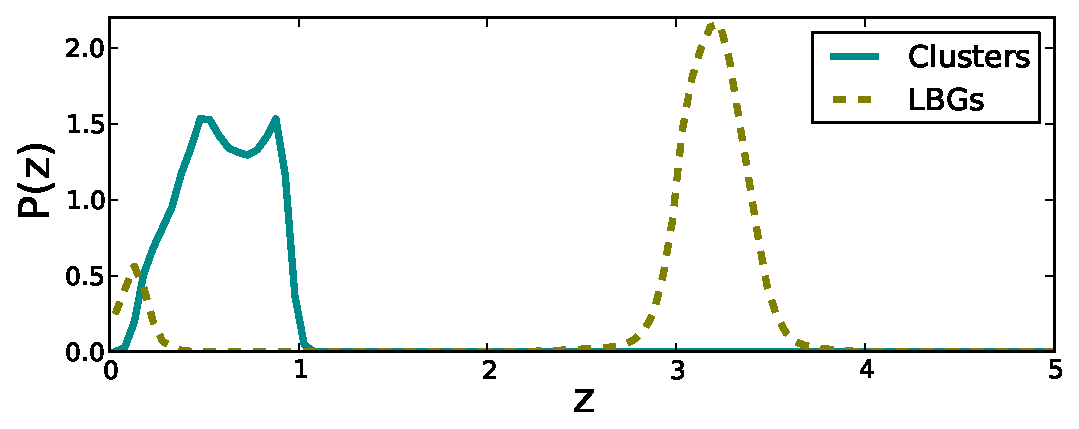
\includegraphics[scale=0.7]{plots_ch3/PofZ_clustersNudrops.eps}
\caption[Redshift Distributions of Clusters and Sources]{Redshift probability distribution functions for the clusters and the LBG sources. Low-redshift contamination of the LBGs will lead to physical clustering correlations where overlap with the cluster redshifts occurs.}
\label{pofz}
\end{center}
\end{figure}

Figure \ref{pofz} shows the redshift probability distributions, $P(z)$, for the clusters and the LBGs. The LBG redshift distribution is based on the stacked posterior $P(z)$ put out by the BPZ redshift code \citep[for details on the CFHTLenS photo-$z$ see][]{Hildebrandt12}. Since the BPZ prior is only calibrated for a magnitude limited sample of galaxies we can not expect the stacked $P(z)$ to reflect the real redshift distribution of the color-selected LBGs. Hence we use the location and shape of the primary (high-$z$) and secondary (low-$z$) peaks but adjust their relative heights separately. This can be done with a cross-correlation technique similar to \citet{Newman08}. Details of this technique will be presented in Hildebrandt et al. (in prep.).

Despite our efforts to avoid contamination, there is obviously some redshift overlap with the clusters. We use the products of the lens and source $P(z)$ to define selection functions, and calculate the expected angular correlations using the code from \citet{Hamana04}. The weighted correlation function that we measure is the sum of the correlations due to lensing magnification and clustering contamination:
\begin{equation}
\mathrm{w}_{\mathrm{opt}}(R,z) = f_{\mathrm{lensing}}\mathrm{w}_{\mathrm{lensing}} + f_{\mathrm{clustering}}\mathrm{w}_{\mathrm{clustering}}.
\end{equation}
Note that $f_{\mathrm{lensing}}+f_{\mathrm{clustering}} \leq 1$, since some of the contaminants may be neither in the background and lensed, nor close enough in redshift to be clustered with the lenses.

The clustering contamination fraction $f_{\mathrm{clustering}}(z)$ for each cluster redshift is defined as the fraction of each source $P(z)$ that lies within 0.1 in redshift (twice the cluster redshift uncertainty). The part of the source $P(z)$ that lies at higher redshift than the lens is then the lensed fraction $f_{\mathrm{lensing}}(z)$, and the part at lower redshift (i.e. in {\it front} of the lens) has no contribution to the signal.

The factor $f_{\mathrm{clustering}}(z)$ itself is generally very small for the LBGs used in this work, only really non-negligible for cluster redshifts $z \sim$ 0.2-0.3, which can be seen in Figure \ref{pofz}. The more significant effect on the estimated masses is that $f_{\mathrm{lensing}}(z) \sim$0.9 across all redshift bins, because about 10\% of the sources are not really being lensed. We tested our results for robustness against uncertainties in the contamination fraction. When we vary the total low-$z$ contamination fraction by $\pm1\sigma$ ($\sim$4\%), the best fit cluster mass estimates remain within the stated error bars.


We explore three ways of determining $\mathrm{w}_{\mathrm{clustering}}$. Because of the weighting applied to LBGs in our measurement (which is optimal for the lensed sources, and should suppress contributions from redshift overlap), there will always be a prefactor of $\langle \alpha-1 \rangle$ in each estimation of clustering. The first method uses the dark matter angular auto-correlation, $\mathrm{w}_{\mathrm{dm}}$, and estimates of the galaxy and cluster bias to calculate:
\begin{equation}
\mathrm{w}_{\mathrm{clustering}}(R,z) = \langle \alpha-1 \rangle b_{l} b_{s} \mathrm{w}_{\mathrm{dm}}(R,z).
\label{model1}
\end{equation}
We set the bias factor for the galaxy contaminants $b_s$=1 for this analysis, which is reasonably consistent with the bias relation of \citet{Seljak04} that is employed for the cluster bias ($b_{l}$).


We also calculate both the 1- and 2-halo terms for NFW halos, w$_{\mathrm{1halo}}$ and w$_{\mathrm{2halo}}$ \citep[again using the code and methods described in][]{Hamana04}. Here the expression for physical clustering takes the form:
\begin{equation}
\mathrm{w}_{\mathrm{clustering}}(R,z) = \langle \alpha-1 \rangle b_{s} \left[\mathrm{w}_{\mathrm{1halo}}(R,z)+\mathrm{w}_{\mathrm{2halo}}(R,z)\right].
\end{equation}
This method requires knowledge of the occupation distribution of the low-$z$ galaxy contaminants in the cluster dark matter halos, which is not well determined. As a first approximation we use the simple power-law form described in \citet{Hamana04},
\begin{equation}
N_g(M) = \begin{cases} (M/M_1)^\alpha & \text{for $M > M_{\mathrm{min}}$} \\ 0 & \text{for $ M < M_{\mathrm{min}}$} \end{cases}.
\end{equation}
Since these parameters are unknown, we use the values for $M_1$ and $\alpha$ measured for galaxies in the SDSS \citep[see Table 3 of][]{Zehavi11}. We choose $M_{\mathrm{min}}$ to correspond to the minimum mass measured for cluster halos, and assume that halos above this mass always host a detected cluster. As a final check, we also ask what the clustering signal would be if every halo above $M_{\mathrm{min}}$ hosted both a cluster and a single low-$z$ galaxy contaminant (so that $N_g = 1$ for $M > M_{\mathrm{min}}$).

This final method yields the largest estimates of $\mathrm{w}_{\mathrm{clustering}}$, and therefore a smaller estimate of cluster masses. The former (using SDSS parameters) gives the highest mass estimates, and the simple biasing approach of Equation \ref{model1} yields intermediate results. We use the range of these results to estimate an uncertainty in mass estimates coming from lack of knowledge about the nature of the low-$z$ galaxies that contaminate our LBG source sample. This additional systematic error affects only the clusters at low redshift, where the source and lens $P(z)$ distributions overlap, and is reported on the mass estimates given in Table 3. All best fit mass values reported in the tables of this work are calculated using the contamination approach of Equation \ref{model1}, since this method relied on the fewest assumptions about the nature of the galaxy contaminants.


Accounting for redshift distributions in this particular source sample effectively means that cluster masses are {\it higher} than one would naively guess by fitting for only the magnification signal. However, note that in a case with more significant redshift overlap, so that $f_{\mathrm{clustering}}$ was large, the opposite statement would be true, and mass estimates that included the full $P(z)$ distribution would be smaller than than the naive magnification-only approach. These are important effects to consider, and future flux magnification studies should be careful to use full redshift distributions in modeling the measured signal.



%ALL CLUSTERS COMBINED PLOT
\begin{figure}
\begin{center}
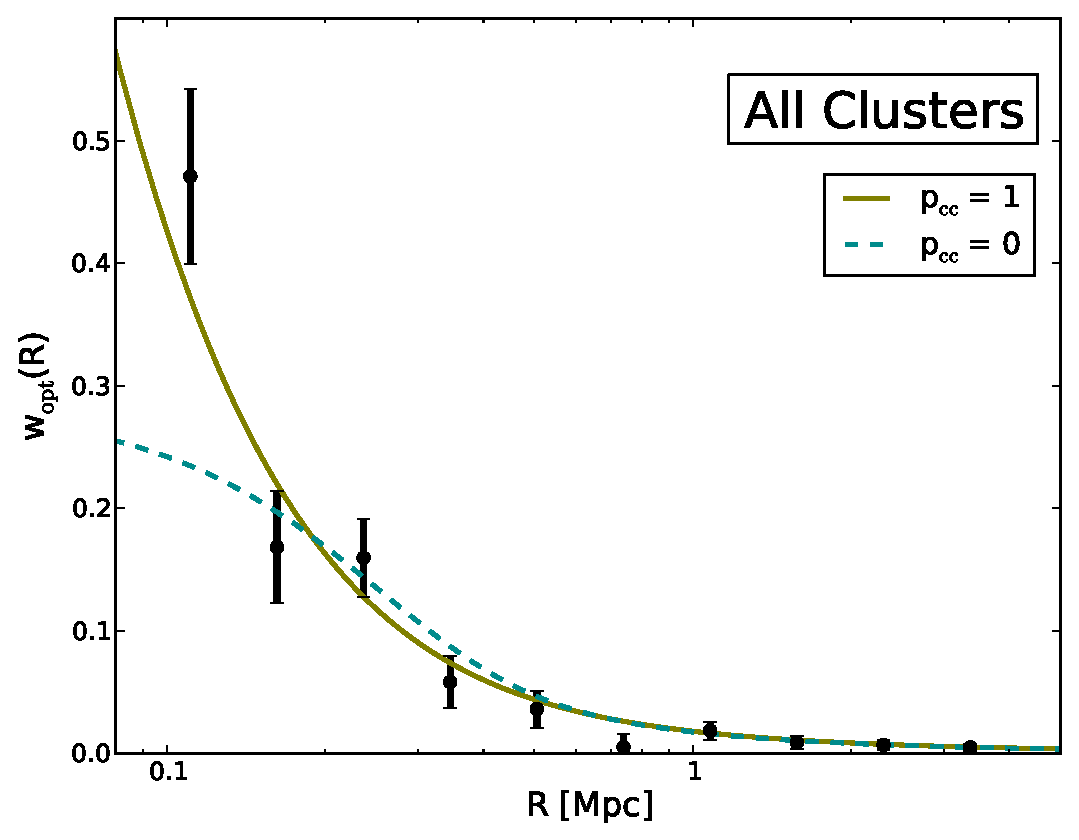
\includegraphics[scale=0.7]{plots_ch3/wopt_allClusters_U.eps}
\caption[Magnification for all Stacked 3D-MF Clusters]{Optimal cross-correlation signal measured for the entire stacked sample of 18,024 clusters. The model fits are both composite-NFW (see text for all terms in the fit). The solid line assumes the clusters are perfectly centered on the peak likelihood of the 3DMF cluster detection, while the dashed line includes the effects of cluster miscentering.}
\label{w_all}
\end{center}
\end{figure}

%-----------------------------------------

\section{Results}
\label{results}

Stacking the entire set of 18,036 clusters gives a total significance of 9.7$\sigma$ for the combined detection, shown in Figure \ref{w_all}. The perfectly centered model is a better fit to the overall measurement, with $\chi^2_{red}$ $\sim$ 1.2, while the miscentered model gives $\chi^2_{red}$ of 2.3. For both models, there are two free parameters ($M_0$ and $\log\beta$), leading to 8 degrees of freedom. To investigate miscentering and mass-richness scaling, we divide the clusters into six richness bins, and measure the optimal cross-correlation in each. 

We measure the characteristic signature of magnification in every richness bin with significances between 4.6 and 5.9$\sigma$. These results are shown in Figure \ref{binned}, where we try fitting both a perfectly centered model ($p_{\mathrm{cc}}=1$) and a model where every cluster is affected by centroid offsets ($p_{\mathrm{cc}}=0$). Details of the fits, including reduced $\chi^2$ and the average of the best fit mass values $\langle M_{200} \rangle$, are given in Table \ref{richtable}.

The lowest mass (richness) bin is not well fit by either model. Overall there is not a strong preference for either perfectly centered ($p_{\mathrm{cc}}=1$) or miscentered ($p_{\mathrm{cc}}=0$) clusters, and both are reasonably good fits. Generally, the miscentered model yields slightly higher masses for the clusters (though it is sensitive to the shape of the data), due to the Gaussian smoothing applied, which lowers the model amplitude in the innermost regions. However this is easily within the uncertainty on the mass estimates, so the results are in agreement.


%PANELS: N200 BINS
\begin{figure}
\begin{center}
%\vspace{1cm}
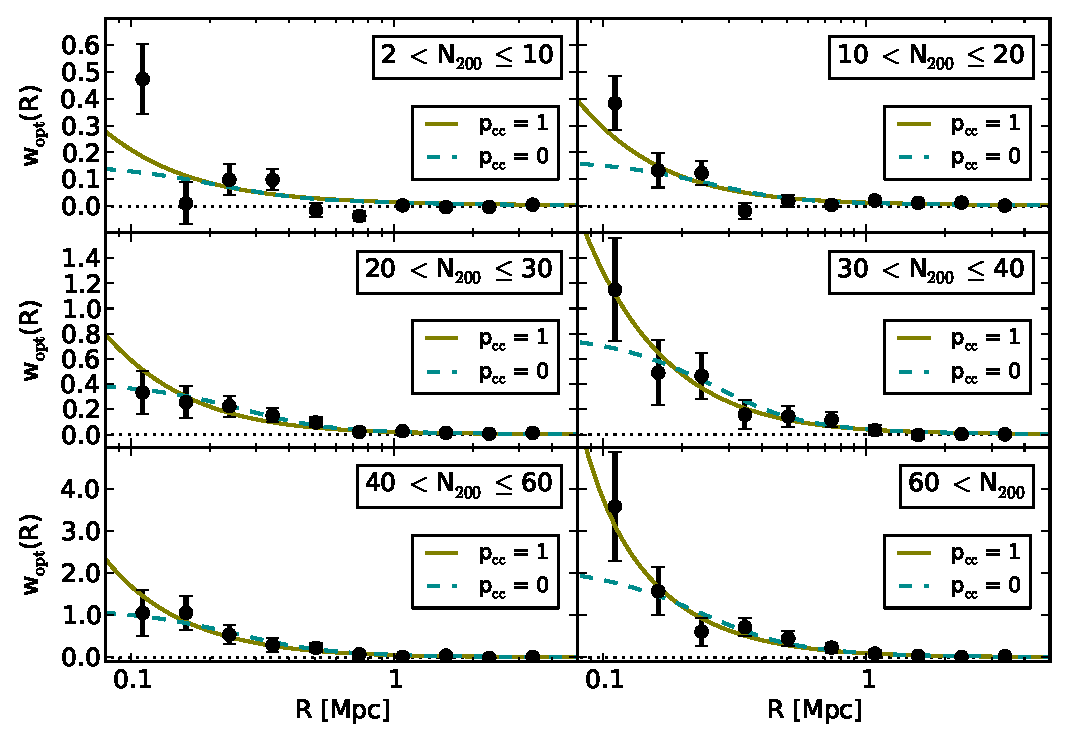
\includegraphics[scale=0.9]{plots_ch3/wopt_panel_fcc0and1_U.eps}
\caption[Magnification for Richness-Binned Clusters]{Optimal cross-correlation signal measured for each $N_{200}$ (richness) bin. Two composite-NFW fits are shown. The solid curve assumes clusters are perfectly centered, while the dashed curve accounts for cluster miscentering, using the gaussian offset distribution modeled in Figure \ref{gauss} and discussed in Section \ref{model}.}
\label{binned}
\end{center}
\end{figure}

The issue of cluster miscentering is interesting in its own right as discussed in Section \ref{centering}. It is tempting to try and fit for the parameter $p_{\mathrm{cc}}$, describing the fraction that are actually correctly centered, or else for the miscentering Gaussian width $\sigma_{\mathrm{offset}}$, as done in \citet{Johnston07}. The issue here is a strong degeneracy between $p_{\mathrm{cc}}$, $\sigma_{\mathrm{offset}}$, and cluster concentration. Increasing the number of clusters that have offset centers produces essentially the same results as leaving $p_{\mathrm{cc}}$ fixed and increasing $\sigma_{\mathrm{offset}}$, an effect that can be mimicked by a lower concentration in the NFW model. We run the risk of overfitting to the results. 

In fact, \citet{Johnston07} found very little constraining power on the miscentering width and the fraction of miscentered MaxBCG clusters, and applied strong priors to these distributions. \citet{George12} performed an extensive weak lensing miscentering study of groups in the Cosmological Evolution Survey (COSMOS), and chose to forgo the additional parameter $p_{\mathrm{cc}}$, as they achieved sufficiently good fits without it. \citet{Mandelbaum08b} performed a lensing analysis of the MaxBCG clusters, and found that including miscentering effects with the \citet{Johnston07} prescription strongly affected the resultant fits for concentration, again asserting the degeneracies of these parameters. \citet{Mandelbaum08b} conclude that this method of accounting for miscentering depends heavily on the mock catalogs from which the input parameters are generated, and in the case of MaxBCG clusters likely overcompensates. 

In a forthcoming paper, we will present weak lensing shear measurements of these clusters, as well as a more detailed investigation of the centroiding. Shear, being proportional to the differential surface mass density, is more affected by offset centers than magnification \citep{Johnston07}, and will be a better probe of miscentering.




%MASS-RICHNESS RELATION
\begin{figure}
\begin{center}
%\vspace{0.5 cm}
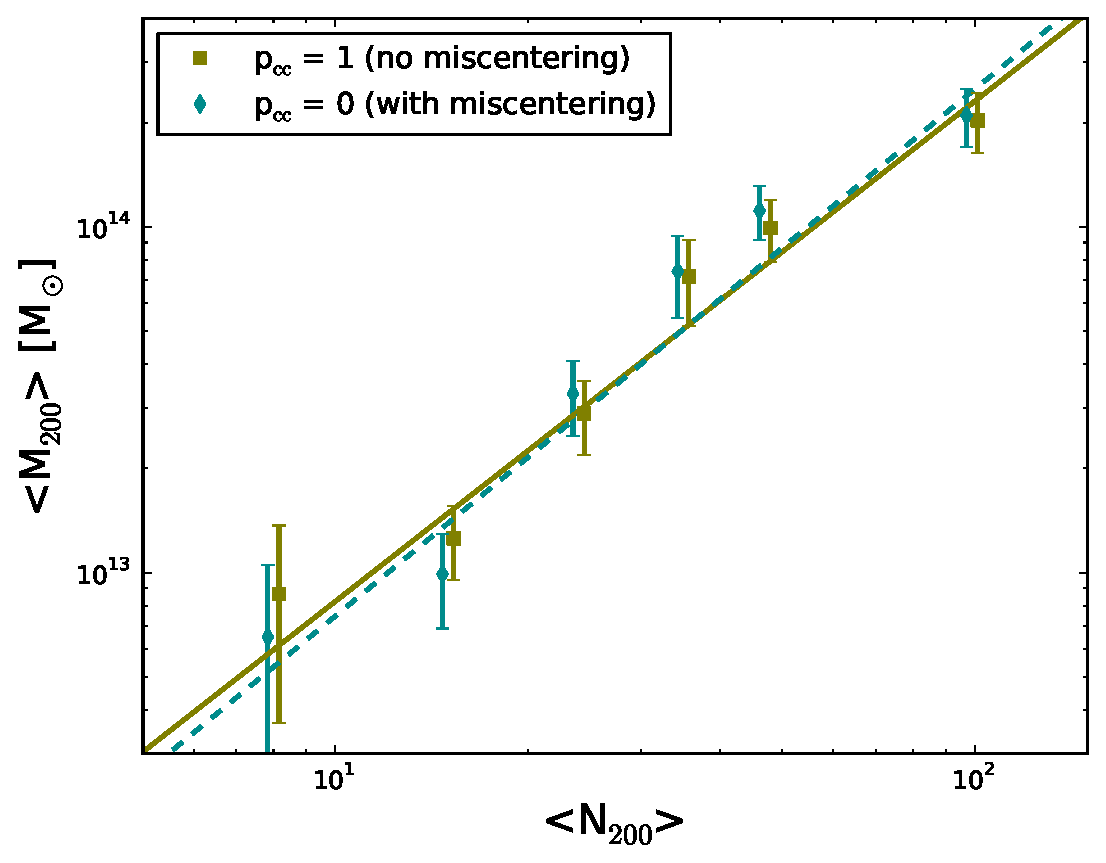
\includegraphics[scale=0.7]{plots_ch3/MassRich_2to1000_U.eps}
\caption[Mass-Richness Relation from Magnification]{Cluster mass-richness relation, using the same $N_{200}$ bins as in Figures \ref{binned}. Power law fits to the data are presented for both cases of with (blue diamonds and dashed line) and without (green squares and solid line) the effects of miscentering. Points are slightly offset horizontally for clarity.}
%\vspace{1 cm}
\label{massrich}
\end{center}
\end{figure}

\subsection{The Mass-Richness Relation}

We observe a prominent scaling of best fit mass to richness, across the six richness bins (although the first two bins do generally have overlapping error bars). We plot this trend in Figure \ref{massrich}, showing the average of the fit masses as a function of average cluster richness in each bin. Note that the distribution of $N_{200}$ in a bin is not uniform, and in the case of the highest richness bin the distribution is highly skewed (see Figure \ref{hist}).

We fit a simple power-law, Equation \ref{mr}, to these points, using the same plotted color and line schemes for perfectly centered and miscentered clusters. For this cluster sample, we find the best fit gives the normalization and slope of the mass-richness relation to be
\begin{equation}
M_0 = (2.3 \pm 0.2) \times 10^{13} M_\odot, \beta = 1.4 \pm 0.1
\end{equation}
for the perfectly centered $p_{\mathrm{cc}}=1$ case, and
\begin{equation}
M_0 = (2.2 \pm 0.2) \times 10^{13} M_\odot, \beta = 1.5 \pm 0.1
\end{equation}
for the miscentered $p_{\mathrm{cc}}=0$ case. The reduced $\chi^2$ are 0.9 and 1.7, respectively (4 degrees of freedom), and there is good agreement between the two different centering scenarios explored here.

%----------------
%LANDSCAPE TABLES
\begin{landscape}

%TABLE FOR RICHNESS-BINNED PLOTS
\begin{table}
  \centering
    \caption[Magnification Results for Richness-Binned Clusters]{Details of fits for richness-binned measurements in Figure \ref{binned}. We list the richness range selected, the number of clusters in that bin, the detection significance, the average richness of the bin, and the mass estimates and reduced $\chi^2$ for both the centered and miscentered models fit to the data. Note that the average mass given is not the value fit itself, but the average of all resulting masses fit using the composite-halo approach discussed in Section \ref{multihalo}.}
    \label{richtable}
    \begin{tabular}{llllllll}
      \hline
       %&  &  &  &   p$_{cc}$=1: & &   p$_{cc}$=0: & \\
      Richness & \# Clusters & Significance & $\langle N_{200} \rangle$ & p$_{cc}$=1: $\langle M_{200} \rangle$ & $\chi^2_{red}$ & p$_{cc}$=0: $\langle M_{200} \rangle$ & $\chi^2_{red}$ \\ \hline
      2 $<N_{200}$ & 18036 & 9.7$\sigma$ & 17 & (2.0$\pm$0.3)$\times10^{13} M_{\odot}$ & 1.2 & (1.8$\pm$0.3)$\times10^{13} M_{\odot}$ & 2.3  \\
      2 $<N_{200}<$ 10 & 4453 & 5.3$\sigma$ & 8 & (0.9$\pm$0.5)$\times10^{13} M_{\odot}$ & 3.0 & (0.7$\pm$0.4)$\times10^{13} M_{\odot}$ & 3.2  \\
      10 $<N_{200}<$ 20 & 9398 & 5.9$\sigma$ & 15 & (1.3$\pm$0.3)$\times10^{13} M_{\odot}$ & 1.6 & (1.0$\pm$0.3)$\times10^{13} M_{\odot}$ & 2.2  \\
      20 $<N_{200}<$ 30 & 2967 & 5.4$\sigma$ & 24 & (2.9$\pm$0.7)$\times10^{13} M_{\odot}$ & 0.7 & (3.3$\pm$0.8)$\times10^{13} M_{\odot}$ & 0.3  \\
      30 $<N_{200}<$ 40 & 695 & 5.0$\sigma$ & 35 & (7$\pm$2)$\times10^{13} M_{\odot}$ & 0.3 & (7$\pm$2)$\times10^{13} M_{\odot}$ & 0.5  \\
      40 $<N_{200}<$ 60 & 351 & 4.6$\sigma$ & 47 & (1.0$\pm$0.2)$\times10^{14} M_{\odot}$ & 0.4 & (1.1$\pm$0.2)$\times10^{14} M_{\odot}$ & 0.3  \\
      60 $<N_{200}$ & 172 & 5.5$\sigma$ & 99 & (2.0$\pm$0.4)$\times10^{14} M_{\odot}$ & 0.5 & (2.1$\pm$0.4)$\times10^{14} M_{\odot}$ & 0.6  \\
      \hline
    \end{tabular}
\end{table}

%TABLE FOR REDSHIFT-BINNED PLOTS
\begin{table}
  \centering
    \caption[Magnification Results for Redshift-Binned Clusters]{Details of fits for redshift-binned measurements in Figure \ref{zbinw}. We list the same bin properties and fits given in Table \ref{richtable}, as well as $f_{clustering}$, which is the total fraction of LBGs expected to lie within $\Delta z \sim$0.1 of the cluster z.}
    \label{ztable}
    \begin{tabular}{lllllllll}
      \hline
      Redshift & $f_{clustering}$ & Clusters & Significance & $\langle N_{200} \rangle$ & p$_{cc}$=1: $\langle M_{200} \rangle$ & $\chi^2_{red}$  & p$_{cc}$=0: $\langle M_{200} \rangle$ & $\chi^2_{red}$ \\ \hline
      $z$ $\sim$ 0.2 & 0.07 & 1157 & 12.5$\sigma$ & 11.6 & (9$\pm$2$\pm$2$^{sys}$)$\times10^{13} M_{\odot}$ & 3.6 & (9$\pm$2$\pm$2$^{sys}$)$\times10^{13} M_{\odot}$ & 3.4  \\
      $z$ $\sim$ 0.3 & 0.02 & 1515 & 8.0$\sigma$ & 14.4 & (6$\pm$1$\pm$1$^{sys}$)$\times10^{13} M_{\odot}$ & 2.2 & (6$\pm$1$\pm$1$^{sys}$)$\times10^{13} M_{\odot}$ & 2.1  \\
      $z$ $\sim$ 0.4 & 3$\times10^{-3}$ & 2242 & 4.6$\sigma$ & 15.2 & (1.9$\pm$0.7)$\times10^{13} M_{\odot}$ & 1.4 & (1.6$\pm$0.7)$\times10^{13} M_{\odot}$ & 1.6  \\
      $z$ $\sim$ 0.5 & 4$\times10^{-4}$ & 2932 & 4.0$\sigma$ & 15.9 & (0.3$\pm$0.4)$\times10^{13} M_{\odot}$ & 1.9 & (0.2$\pm$0.5)$\times10^{13} M_{\odot}$ & 1.9  \\
      $z$ $\sim$ 0.6 & 1$\times10^{-4}$ & 2455 & 4.6$\sigma$ & 18.0 & (2.2$\pm$0.8)$\times10^{13} M_{\odot}$ & 1.5 & (2.0$\pm$0.8)$\times10^{13} M_{\odot}$ & 1.6  \\
      $z$ $\sim$ 0.7 & 2$\times10^{-5}$ & 2331 & 4.5$\sigma$ & 19.3 & (1.2$\pm$0.7)$\times10^{13} M_{\odot}$ & 1.7 & (1.1$\pm$0.7)$\times10^{13} M_{\odot}$ & 1.9  \\
      $z$ $\sim$ 0.8 & 2$\times10^{-5}$ & 2364 & 4.9$\sigma$ & 19.9 & (2.5$\pm$0.9)$\times10^{13} M_{\odot}$ & 1.5 & (2.2$\pm$0.9)$\times10^{13} M_{\odot}$ & 1.7  \\ 
      $z$ $\sim$ 0.9 & 2$\times10^{-5}$ & 3040 & 2.6$\sigma$ & 17.6 & (0.5$\pm$0.5)$\times10^{13} M_{\odot}$ & 0.6 & (0.3$\pm$0.6)$\times10^{13} M_{\odot}$ & 0.8  \\
      \hline
    \end{tabular}
\end{table}
\end{landscape}
%----------------


It is difficult to directly compare the results for the mass-richness relation in this work to other studies. The main reason is that the richness $N_{200}$ we use is different than other definitions, which often count only red-sequence galaxies. Some uncertainty exists in the measure of richness as well, which we do not include in the analysis. Alternative measures of cluster richness would yield different scaling relations. Another factor is the cluster sample, which was compiled using a novel cluster-finder, and may well have different characteristics than other samples in the literature. In a follow-up paper we will present a shear analysis of the CFHTLenS clusters, and compare the mass-richness relation obtained using that complementary probe of halo mass.


\subsection{Redshift Binning}
\label{zbin}

%Z BINNED HISTOGRAM
\begin{figure}
\begin{center}
%\vspace{1 cm}
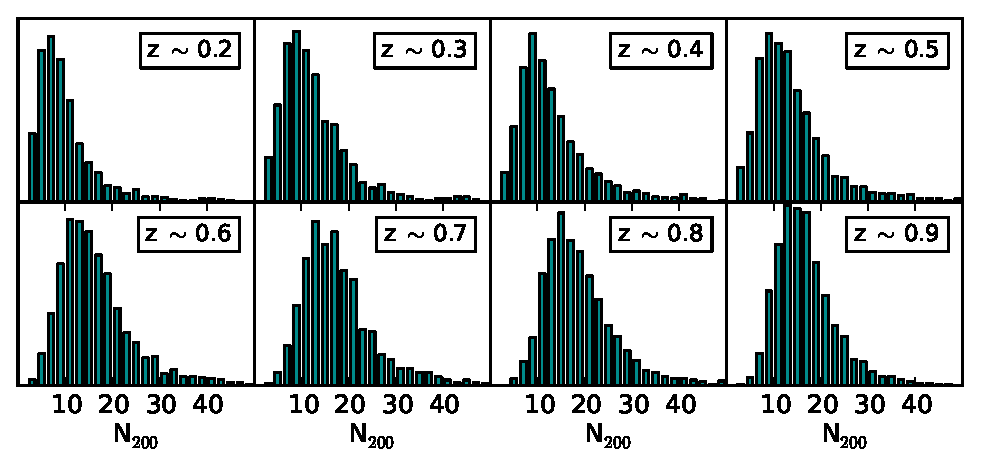
\includegraphics[scale=1.0]{plots_ch3/zbin_histograms.eps}
\caption[Richness Distributions in Redshift Bins]{$N_{200}$ distributions as a function of cluster redshift.}
%\vspace{1 cm}
\label{zbinhist}
\end{center}
\end{figure}

Finally, we investigate the magnification as a function of redshift. We stack clusters of all richnesses, at each redshift in the catalog, $0.2 \leq z \leq 0.9$, and measure the optimal correlations in each. This is displayed in Figure \ref{zbinw}. We observe a steady decrease in measured signal as the cluster redshift increases from $z \sim$0.2 to 0.5, then roughly consistent measurements from 0.6$\leq z \leq$0.8, followed by rather low signal at $z \sim$0.9. 

The $N_{200}$ distributions in Figure \ref{zbinhist} show that these trends cannot be caused by deviations in richness between these different cluster redshifts. This is difficult to reconcile with the clear mass-richness scaling observed when all redshifts are combined. Table 3 shows that detection significance for each reshift bin is more tightly linked to mass than the $\langle N_{200} \rangle$. Perhaps the richness estimates used in this work are not optimized for use as a mass proxy at all redshifts. Another possibility is that we have not correctly accounted for redshift overlap between samples. If the contamination fraction is higher than estimated, this could lead to a boost in correlation strength at low redshift, as well as a depletion at higher redshift. However it is still very difficult to explain the anomalously low measurement at intermediate redshift, $z \sim$0.5, with this reasoning.

One factor that we have not accounted for is possible cluster false detections in our sample. Since 3D-MF was optimized to produce cluster catalogs that are as complete as possible, false detection rates could be quite high. In particular, we would expect these rates to increase at high redshift, which would also weaken those measured correlations. We note in particular that cluster redshift bins $z \sim$ 0.5 and 0.9, which yield relatively low cluster masses, are seen in Figure \ref{pofz} to have excess numbers of detected clusters, possibly an indication of higher false detection rates at these redshifts.


%Z BINNED WOPT
\begin{figure}
\begin{center}
%\vspace{1 cm}
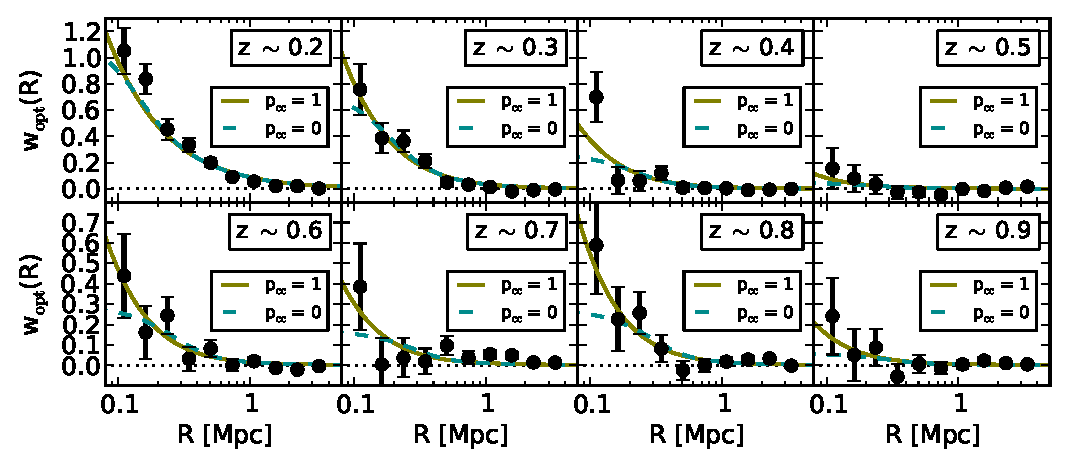
\includegraphics[scale=0.9]{plots_ch3/wopt_z_panels_U.eps}
\caption[Magnification for Redshift-Binned Clusters]{Optimal correlation for clusters binned in redshift.}
%\vspace{1 cm}
\label{zbinw}
\end{center}
\end{figure}
%\vspace{1 cm}


%-----------------------------------------

\section{Conclusions}
\label{conc}
We present the most significant magnification-only cluster measurement to date, at 9.7$\sigma$. A sample of 18,036 cluster candidates has been detected using the 3D-MF technique in the $\sim$154 deg$^2$ CFHTLenS survey. In this analysis we have investigated the mass of cluster dark matter halos, from flux magnification, as a function of both richness and redshift. A forthcoming paper will present the weak lensing shear analysis of these clusters as well.

We fit a composite-NFW model that accounts for the full redshift and mass ranges of the cluster sample, as well as redshift overlap with low-$z$ source contaminants, cluster halo miscentering, and the 2-halo term. We find that the entire cluster sample is marginally better fit by the model that does not include miscentering, but do not see a strong preference either way across richness bins. In the future, shear measurements, which are more sensitive to miscentering, may illuminate this aspect of the investigation.

We observe a strong scaling between measured mass and cluster richness, and fit a simple power-law relation to the data. The two miscentering models explored in this work yield consistent values for the normalization and slope of the mass-richness relation.

We have attempted to account for the contamination of our background sources with low-$z$ galaxies. This is a serious systematic effect for magnification, as redshift overlap between lenses and sources will lead to physical clustering correlations, swamping the lensing-induced correlations that we want to measure. We use the full stacked redshift probability distributions for the lens and source populations, and include the expected clustering contribution in our model. In spite of this we see unexpected features in the redshift-binned measurements. Part of the reason could come from cluster false detections, which can be high for the 3D-MF method which is optimized for completeness. Another contribution could come from errors in the source redshift distributions. Accounting for redshift overlap is imperative if significant overlap exists between the lens and source distributions, or else mass estimates can end up very biased.

This is the first analysis presented of the 3D-MF clusters in CFHTLenS, but much more science is left to do with the sample. In particular, a more thorough investigation of the miscentering problem will be carried out in the forthcoming shear analysis, where it will be possible to compare different candidate centers. Another interesting question is whether dust can be detected on cluster scales by simulataneously measuring the chromatic extinction along with flux magnification. Finally different background source samples may be employed to improve signal-to-noise, but only if their redshift distributions can be well determined. We leave these tasks to future work.

This work has been an important step in the development of weak lensing magnification measurements, and the progression from signal detection to science. Many upcoming surveys will benefit from the inclusion of magnification in their lensing programs, as the technique offers a very complimentary probe of large scale structure. Since measuring flux magnification is not a strong function of image quality, it is especially useful for ground-based surveys which must deal with atmospheric effects. Next generation surveys like the Large Synoptic Survey Telescope (LSST), the Wide-Field Infrared Survey Telescope (WFIRST), and Euclid, will have greater numbers of sources, and improved redshift probability distribution estimates, so we can expect future magnification studies to yield important contributions to weak lensing science and cosmology.


 %CFHTLenS Magnification
\chapter{CFHTLenS: A Weak Lensing Shear Analysis of the 3D-Matched-Filter Galaxy Clusters}


%\begin{abstract} 
We present the cluster mass-richness scaling relation calibrated by a weak lensing analysis of $>$18000 galaxy cluster candidates in the Canada-France-Hawaii Telescope Lensing Survey (CFHTLenS). Detected using the 3D-Matched-Filter cluster-finder of Milkeraitis et al., these cluster candidates span a wide range of masses, from the small group scale up to $\sim10^{15} M_{\odot}$, and redshifts 0.2 $\leq z\leq$ 0.9. The total significance of the stacked shear measurement amounts to 54$\sigma$. We compare cluster masses determined using weak lensing shear and magnification, finding the measurements in individual richness bins to yield 1$\sigma$ compatibility, but with magnification estimates biased low. This first direct mass comparison yields important insights for improving the systematics handling of future lensing magnification work. In addition, we confirm analyses that suggest cluster miscentring has an important effect on the observed 3D-MF halo profiles, and we quantify this by fitting for projected cluster centroid offsets, which are typically $\sim$ 0.4 arcmin. We bin the cluster candidates as a function of redshift, finding similar cluster masses and richness across the full range up to $z \sim$ 0.9. We measure the 3D-MF mass-richness scaling relation $M_{200 } = M_0 (N_{200} / 20)^\beta$. We find a normalization $M_0 \sim (2.7^{+0.5}_{-0.4}) \times 10^{13} M_{\odot}$, and a logarithmic slope of $\beta \sim 1.4 \pm 0.1$, both of which are in 1$\sigma$ agreement with results from the magnification analysis. We find no evidence for a redshift-dependence of the normalization. The CFHTLenS 3D-MF cluster catalogue is now available at \url{cfhtlens.org}.
%\end{abstract}


%==========================================================================

\section{Introduction}
\label{intro}
The evolution of large scale structure is overwhelmingly driven by the invisible components which make up the majority of the present day energy density of the Universe. In order to probe these structures we are forced to rely on biased tracers of the underlying density field that we can actually observe, such as galaxies. Large galaxy cluster surveys are invaluable in providing sufficient statistics for classifying and analysing the most massive gravitationally bound systems that have had time to form in our cosmic history. In addition to providing a cosmological probe, they are interesting laboratories for the evolution of individual galaxies and the intracluster medium \citep{Voit05}.

Several methods have been developed for identifying clusters in optical galaxy surveys, including the red sequence technique \citep{Gladders00}, density maps \citep{Adami10}, redMaPPer \citep{Rykoff14}, and matched-filter methods \citep{Postman96}. An extension of the latter, 3D-Matched-Filter (3D-MF), is described in \citet{Milkeraitis10} and used in this work. This cluster finder attempts to circumvent the common issue of line-of-sight projections by using photometric redshift information to identify clusters in redshift slices. Beyond the use of photometric redshifts, 3D-MF does not apply any additional colour-selection criteria for identifying clusters (e.g. that cluster members must fall on the red sequence). A similar algorithm tuned for galaxy groups was introduced by \citet{Gillis11}. Every cluster-finding technique will pick out clusters with somewhat distinct characteristics because of different assumptions that are made in the algorithm, and it is therefore important to characterize and contrast independent samples of clusters \citep{Milkeraitis10}.

Among the broad array of analysis tools employed by the galaxy cluster research community, gravitational lensing is a crucial technique for obtaining masses and density profiles, independent of assumptions regarding cluster dynamical state. In the weak regime, lensing provides robust measurements of stacked cluster samples (and individual masses for very massive clusters), affording a statistical view of average galaxy cluster properties \citep{Hoekstra13}. The majority of weak lensing studies measure the shear, or shape distortion, of lensed source galaxies. The complementary magnification component of the lensing signal has more recently been measured with increasing precision \citep{Scranton05,Hildebrandt09b,Ford12,Ford14,Morrison12,Hildebrandt13,Bauer14}, and has been combined with shear in joint-lensing analyses \citep{Umetsu11,Umetsu14}. When combined with other cluster observables, lensing yields useful scaling relations that can be extrapolated with some caution to wider cluster populations, or cross-examined to characterize intrinsic disparities that may distinguish catalogues compiled using different cluster-finding techniques \citep{Hoekstra07,Johnston07,Leauthaud10,Hoekstra12,Covone14,Oguri14}.

Section 2 of this paper describes the data, Section 3 gives the formalism of the weak lensing measurement, and Section 4 presents the results. We then discuss and compare our findings to other results, including our previous magnification measurements of the same lens sample, in Section 5. We finish with conclusions in Section 6. Throughout this work we use a concordance $\Lambda$ cold dark matter cosmology with $\Omega_M$ = 0.3, $\Omega_{\Lambda}$ = 0.7, and H$_0$ = 70 km/s/Mpc.

%==========================================================================

\section{Data}
\label{data}

%-----------------------------------------------

\subsection{The Canada-France-Hawaii Telescope Legacy Survey Wide}

The Canada-France-Hawaii Telescope Legacy Survey (CFHTLS) is a multi-component optical survey conducted over more than 2300 h in 5 yr ($\sim450$ nights) using the wide field optical imaging camera MegaCam on the CFHT's imaging system MegaPrime. The Wide survey is composed of four patches ranging from 25-72 deg$^2$, together totalling an effective survey area of $\sim$ 154 deg$^2$. The data were acquired through five filters: $u$*, $g'$, $r'$, $i'$, $z'$, and has a 5$\sigma$ point source $i'-$band limiting magnitude of 24.5. The breadth of CFHTLS-Wide was intended for the study of large scale structure and matter distribution in the Universe.

The CFHTLS-Wide optical multi-colour catalogues used in this work were created from stacked images of the aforementioned Wide fields \citep[see][for details on the data processing and multi-colour catalogue creation]{Erben09, Hildebrandt09a, Hildebrandt12, Erben13}. Basic photometric redshift ($z_{\mathrm{phot}}$) statistics were determined by \citet{Hildebrandt12}. In this work we restrict ourselves to a redshift range of 0.1 $\leq z \leq$ 1.2, which has outlier rates $\leq$ 6\% and scatter $\sigma \leq$ 0.06.

%----------------------------------------------

\subsection{CFHTLenS Shear Catalogue}

The Canada-France-Hawaii Telescope Lensing Survey (CFHTLenS) reduced CFHTLS-Wide data for weak lensing science applications \citep{Heymans12,Erben13}. Many factors affect high-precision weak lensing analyses, including correlated background noise, PSF measurement, and galaxy morphology evolution for example \citep[for a more detailed list and study, see][]{step2,Heymans12}. The efforts of CFHTLenS have led to new reduction methodologies with reduced systematic errors and a more thorough understanding of the PSF and its variation in the CFHTLS-Wide images. As part of this pipeline, {\em lens}fit was used to measure galaxy shapes \citep{Miller13}, which were tested for systematics in \citet{Heymans12}. The galaxy shear measurements and photometric redshifts used in this work are publicly available.\footnote[1]{\url{www.cfhtlens.org}; Data products are made available at \url{http://www.cadc-ccda.hia-iha.nrc-cnrc.gc.ca/community/CFHTLens/query.html}}
%{www.cfhtlens.org; Data products are made available at http://www.cadc-ccda.hia-iha.nrc-cnrc.gc.ca/\-community/\-CFHTLens/\-query.html}
%\footnote[1]{www.cfhtlens.org; Data products are made available at http://www.cadc-ccda.hia-iha.nrc-cnrc.gc.ca/\-community/\newline CFHTLens/\-query.html}

%----------------------------------------------

\subsection{3D-MF Clusters}\label{3DMF}

Here we give a brief overview of the 3D-MF galaxy cluster-finding algorithm. For additional background and details on the algorithm, including extensive testing on the Millennium Simulation data set, and information on the completeness and purity of a 3D-MF derived galaxy cluster catalogue, the reader is directed to \citet{Milkeraitis10}.

3D-MF searches survey data for areas that maximally match a given luminosity and radial profile for a fiducial galaxy cluster, similar to the technique used by \citet{Postman96}.  For the luminosity profile we use an integrable Schechter function, given by
\begin{equation}
\Phi(M)=0.4 \ \ln(10) \ \Phi^* 10^{0.4(\alpha + 1)(M^*-M)} \exp \left[ -10^{0.4(M^*-M)} \right],
\end{equation}
where $\Phi$ is the galaxy luminosity function, $\Phi^*$ sets the overall normalization, $M$ is absolute magnitude, $M^*$ is a characteristic absolute magnitude, and $\alpha$ is the faint end slope of the luminosity function. As discussed in \citet{Milkeraitis10}, the multiplicative term, exp$[-10^{0.4(M^{*}-M)}]$, keeps this function from diverging when $\alpha < -1$ and $M < M^*$. For the radial profile we use a truncated Hubble profile, given by
\begin{equation}
P \left ( \frac{r}{r_c} \right )=\frac{1}{\sqrt{1+ \left ( \frac{r}{r_c} \right ) ^2}} - \frac{1}{\sqrt{1+ \left ( \frac{r_{co}}{r_c} \right ) ^2}},
\end{equation}
where $r_c$ is the cluster core radius, and $r_{co} \gg r_c$ is the cutoff radius. In an attempt to match both of the above profiles, 3D-MF creates likelihood maps of the sky survey area. Peaks in this map are possible cluster detections, and are each assigned a significance $\sigma_{\rm cl}$ relative to the background signal \citep[$\sigma_{\rm cl}$ is calculated using Equation 5 of][which the reader is referred to for more details]{Milkeraitis10}. The cluster centres are defined to be the locations of the likelihood peaks; see Section \ref{sec:miscentring} for how uncertainties in the centres are dealt with.

An important characteristic of this cluster-finding algorithm is the fact that the described process is carried out in discrete redshift bins to avoid spurious false-detections due to line-of-sight projections. 3D-MF was run on the CFHTLS-Wide catalogues with redshift slices of width $\Delta z = 0.2$, which are then shifted by 0.1, and the finder is run again on the overlapping redshift slices. Clusters are assigned a final redshift estimate (of bin width $\Delta z = 0.1$) by using the centre of the slice that maximizes cluster detection significance. 3D-MF was run using the same run-time parameters listed in table~2 in \citet{Milkeraitis10}, with the exception of an absolute $i'-$band magnitude of $M^*_{i'-\mathrm{band}}=-23.22 \pm 0.01$ and slope of the Schechter luminosity function, $\alpha=-1.04 \pm 0.01$, derived from the Wide data \citep{MMthesis11}.

Excluding possible multiple detections, a total of 22,694 galaxy cluster candidates were found in the CFHTLS-Wide data set with detection significance $\sigma_{\rm cl} \ge 3.5$. Using 3D-MF's multiple detection criteria, there were $34.4\%$ additional duplicate detections of galaxy clusters. This is comparable to the $\sim 36\%$ multiple detection rate found from Millennium Simulation tests and $37.6\%$ found in the CFHTLS-Deep galaxy cluster catalogue in \citet{Milkeraitis10}. Using the Millennium Simulation, \citet{Milkeraitis10} determined that there are potentially $\sim 16\%-24\%$ false positives in 3D-MF-derived galaxy cluster catalogues, distributed mostly in the lower significance ranges \citep[see Table~3 in][]{Milkeraitis10}.

Following the 3D-MF methodology for galaxy cluster catalogue generation, the significance of galaxy cluster detections was used to select the best galaxy cluster candidate among multiple detections, and the remaining multiple detections were rejected from the analysis. A single detection of each cluster candidate then makes up the CFHTLS-Wide galaxy cluster candidate catalogue. We restrict our analysis herein to a cluster redshift range of 0.2 $\leq z \leq$ 0.9, where 3D-MF detections are the most reliable.

%MASS-SIG RELATION
\begin{figure}
\begin{center}
%\vspace{0.2cm}
  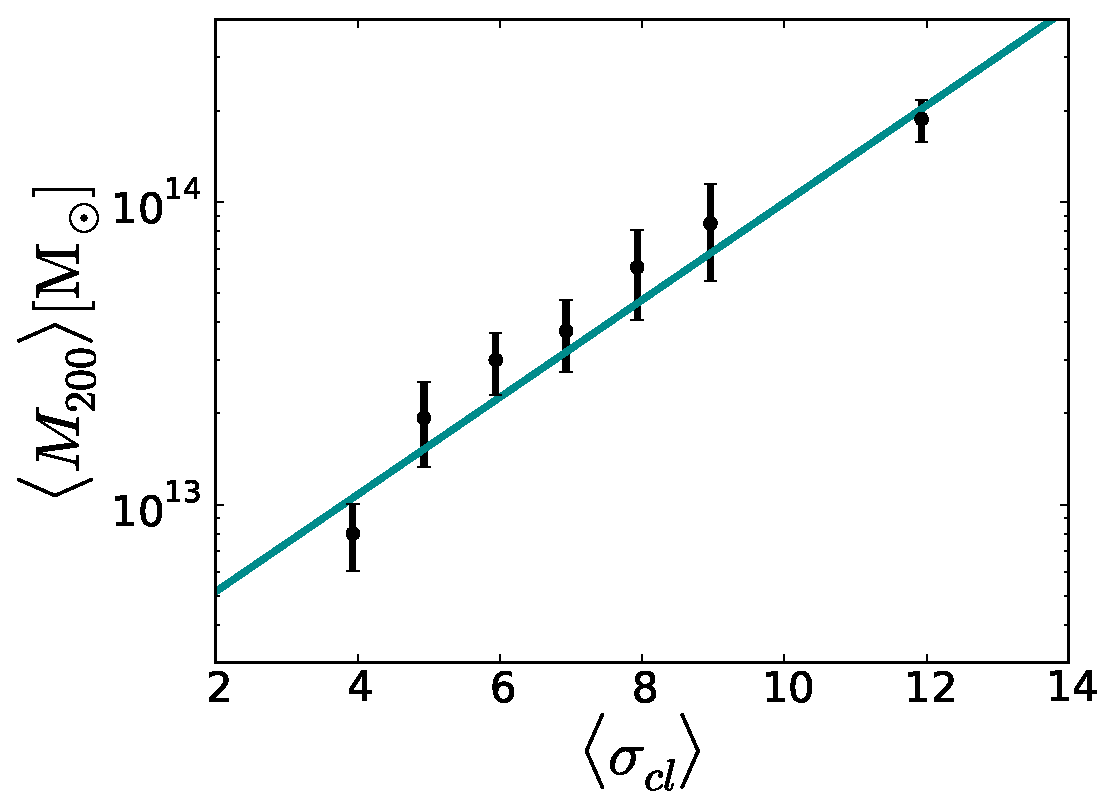
\includegraphics[scale=0.7]{plots_ch4/MassSig_relation.eps}
  \caption[Mass-Significance Relation]{Scaling of shear-measured mass $M_{200}$ with the 3D-MF cluster detection significance $\sigma_{\rm cl}$. Since we find significance to be a good proxy for mass, we use the derived mass-significance relation to estimate a radius $r_{200}$ for each cluster candidate, within which we count galaxies for richness $N_{200}$, as described in the Section \ref{3DMF}.}
\label{plot:masssig} %labels must be after caption
\end{center}
\end{figure}

%CLUSTER HISTOGRAMS
\begin{figure}
\begin{center}
\vspace{0.5cm}
  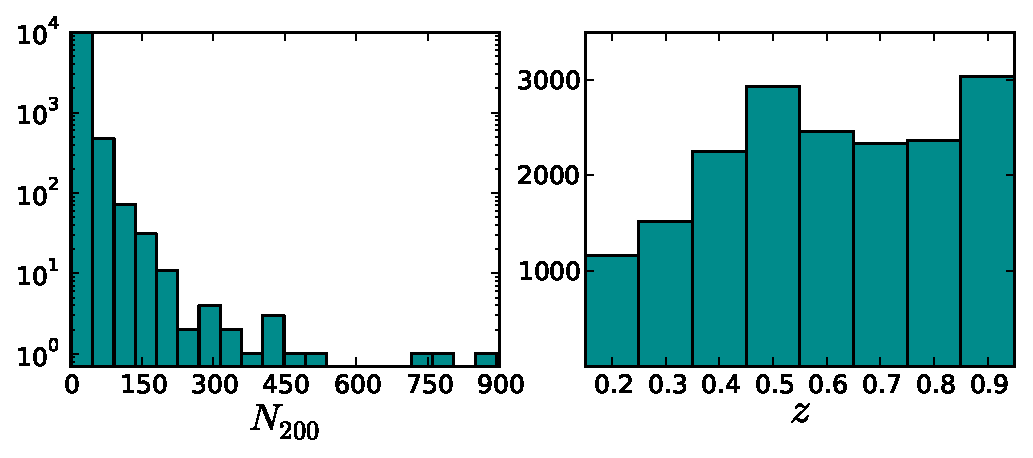
\includegraphics[scale=0.9]{plots_ch4/hists_N200_z_NoGaps.eps}
  \caption[Richness and Redshift Distributions of 3D-MF Clusters]{Number of 3D-MF cluster candidates as a function of richness $N_{200}$ and redshift $z$.}
\label{plot:hists}
\end{center}
\end{figure}

In \citet{Ford14}, we described our method of calculating richness for each of these candidate clusters. $N_{200}$ is defined to be the number of member galaxies brighter than absolute magnitude $M_i \ge -19.35$, which is chosen to match the limiting magnitude at the furthest cluster redshift that we probe ($N_{200}$ is background-subtracted; there is no correction for passive evolution). To be considered a cluster member, a galaxy must lie within a projected radius $R_{200}$ of a cluster centre, and have $\Delta z < 0.08(1+z)$ \citep[based on the photometric errors of the CFHTLenS catalogue; for details regarding $N_{200}$ see][]{Ford14}. $R_{200}$ is defined as radius within which the average density is 200 times the critical energy density of the Universe ($M_{200}$ is the total mass inside $R_{200}$), and in this work has been re-estimated from the data as follows. 

Initially cluster candidates were stacked in bins of cluster detection significance $\sigma_{cl}$, which was found to correlate well with the amplitude of the measured shear profiles, and therefore with mass (see Figure \ref{plot:masssig}). These preliminary masses were estimated using the same method described in Section \ref{method}. A new mass-significance relationship,
\begin{equation}
\label{eqn:masssig}
\mathrm{log}\left[ \frac{M_{200}^{\rm prelim}}{M_{\odot}} \right] = \left( 0.161^{+0.006}_{-0.009} \right) \sigma_{\rm cl} + 12.39^{+0.05}_{-0.08},
\end{equation}
was derived from this result and the preliminary mass values converted into the corresponding radii, which were used to count galaxies for richness ($\sigma_{\rm cl} \rightarrow M_{200}^{\rm prelim} \rightarrow R_{200} \rightarrow N_{200}$). Compared with the richness estimates used in \citet{Ford14}, which were based on a preliminary shear analysis using a more basic cluster modelling approach \citep{MMthesis11}, the updated richnesses are larger in most cases (see the Full Model description in Section \ref{sec:halomodel} for improvements). For the log-normal curve in Figure \ref{plot:masssig}, as well as for all models fit in this work, the best fit is the curve that minimizes $\chi^2$, using a downhill simplex algorithm to search parameter space.

%N200-SIG RELATION
\begin{figure}
\begin{center}
\vspace{0.2cm}
  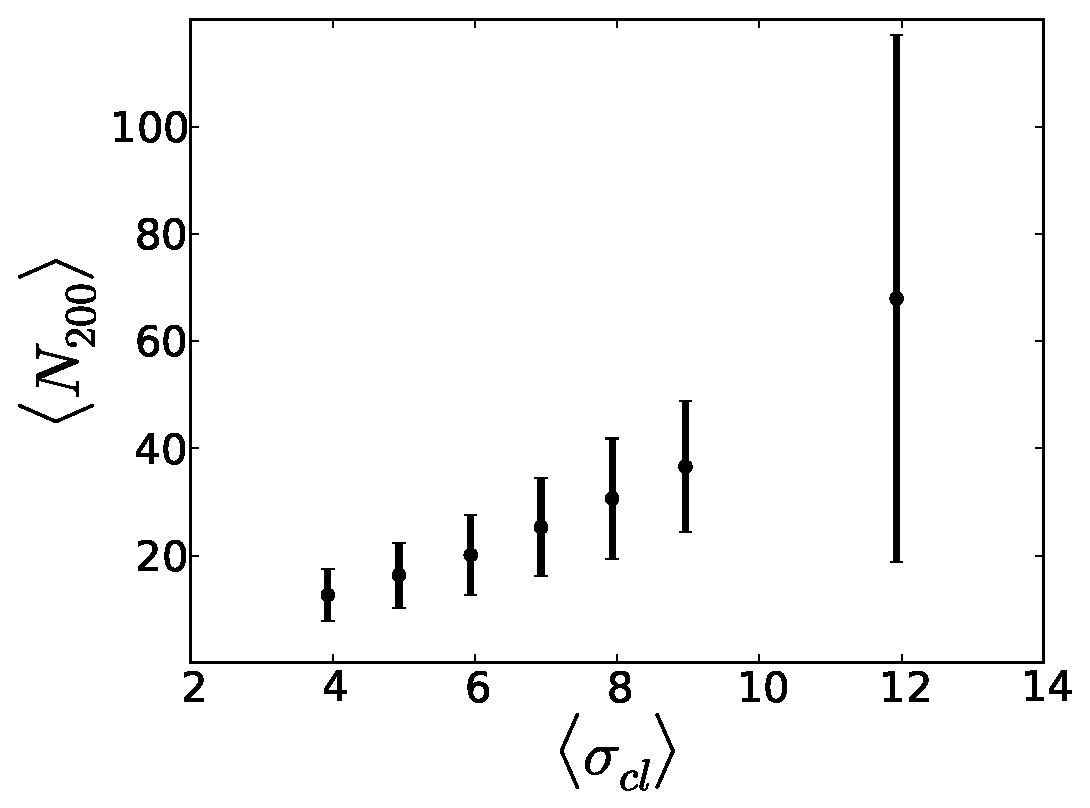
\includegraphics[scale=0.7]{plots_ch4/N200vsSig.eps}
  \caption[Richness-Significance Scaling]{Scaling of richness $N_{200}$ with the 3D-MF cluster detection significance $\sigma_{\rm cl}$. Error bars denote the standard deviation of the ensemble of $N_{200}$ values in each $\sigma_{\rm cl}$ bin. Since $N_{200}$ is estimated using individual cluster radii calculated from the mass-significance relation (Equation \ref{eqn:masssig}), this figure confirms what we would expect -- a strong scaling between richness and significance.}
\label{plot:n200sig} %labels must be after caption
\end{center}
\end{figure}

Cluster candidates used in this work are required to have at least $N_{200} > 2$, and a detection significance $\ge 3.5$. The richness and redshift distributions are summarized in Figure \ref{plot:hists}. Figure \ref{plot:n200sig} shows the relative scaling between richness and detection significance. The final catalogue contains the same 18036 cluster candidates used in \citet{Ford14}, now with updated richness estimates based on the shear mass-significance scaling just described. There are also 20 additional low-significance cluster candidates whose revised $N_{200}$ now survive the cuts -- these systems have negligible impact on the overall results, but do increase the total number of clusters to 18056. The full 3D-MF catalogue is available at \url{cfhtlens.org}.  


%==========================================================================

\section{Method}
\label{method}
%----------------------------------------------

\subsection{Stacking Galaxy Clusters}

The mass of a galaxy cluster can be determined by measuring shear in binned annuli out from the cluster centre, and fitting this with a theoretical density profile. For the most massive galaxy clusters, this is relatively straightforward. However, for most galaxy clusters (especially given the high number of lower mass galaxy cluster candidates explored in this work), the background noise overwhelms the measurable shear.  Fortunately, stacking many individual galaxy clusters together improves the signal-to-noise ratio, enabling the measurement of a statistically significant signal, averaged over a cluster ensemble.

To obtain a meaningful average for a property of an ensemble of galaxy clusters, similar clusters must clearly be chosen for a stack. It is desirable to stack clusters of very similar mass (and thus clusters of roughly the same size and profile), as an average mass measurement of the cluster stacks is the goal. In fitting models to the stacked weak lensing measurements in this work, we assume that the haloes are spherical on average. However, recent studies have explored halo orientation bias in simulations, demonstrating that optically-selected clusters will tend to be aligned along the line-of-sight, and this effect could lead to our mass estimates being biased high by $3-6$\% \citep{Dietrich14}.

For this analysis, the cluster candidates are stacked in bins of richness $N_{200}$ as well as redshift, identical to those used in \citet{Ford14}. The overall approach is conceptually very similar to that used in galaxy-galaxy lensing \citep[see][]{Velander14}, except we replace the galaxy lenses with cluster lenses.

%----------------------------------------------

\subsection{Measuring $\Delta\Sigma$}
\label{sec:measure}

We measure the radial profile of the tangential shear, $\gamma_t(R)$, around each cluster candidate in bins of projected {\it physical} distance $R$, extending from 0.09 to 5 Mpc. The logarithmically-spaced radial bins are chosen to match those used in \citet{Ford14}, which we compare results to in Section \ref{sec:magn}, and the resulting mass measurements are insensitive to small adjustments in the innermost radii. To select background galaxies for measuring shear, we use their redshift probability distributions $P(z_s)$, where $z_s$ is the source redshift. Relative to a given cluster redshift ($z_l$), we require both that (1) the peak of a galaxy's $P(z_s)$ distribution is at higher redshift, and (2) at least 90\% of a galaxy's $P(z_s)$ is at higher redshift. The second requirement is designed to account for the occasional galaxy with an odd $P(z_s)$, which may peak at high redshift (and so would be included in many conventional shear analyses), but could perhaps have a non-negligible tail extending to low $z$, or even be bimodal.

From the individual shear profiles we construct $\Delta\Sigma$, the differential surface mass density, for each stacked cluster candidate sample: 
\begin{equation}
\label{eqn:deltasig}
\Delta\Sigma(R) \equiv \overline{\Sigma}(<R)-\Sigma(R) = \langle \gamma_t(R) \rangle \Sigma_{\mathrm{crit}}.
\end{equation}
Here $\Sigma(R)$ is the surface mass density of a lens, and $\Sigma_{\mathrm{crit}}$ is the critical surface mass density, which depends on the geometry of the lens-source pairs. It is given by
\begin{equation}
\label{eqn:sigcrit}
\Sigma_{\mathrm{crit}} = \frac{C^2}{4 \pi G} \frac{D_s}{D_l D_{ls}},
\end{equation}
where $C$ is the speed of light and $D_s$, $D_l$, and $D_{ls}$, are the angular diameter distances to the source, to the lens, and between the lens and source, respectively. 

In computing $\Sigma_{\mathrm{crit}}$ for {\it each lens-source pair}, we treat the individual lens $z_l$ as fixed, and integrate over the full source $P(z_s)$, for $z_s > z_l$, to compute the distances:
\begin{equation}
D_s = \int_{z_l}^{\infty} D_{ang}(0,z_s) P(z_s) {\rm d}z_s
\end{equation}
\begin{equation}
D_{ls} = \int_{z_l}^{\infty} D_{ang}(z_l,z_s) P(z_s) {\rm d}z_s
\end{equation}
Here $D_{ang}$ is the angular diameter distance between two redshifts (and $D_l$ is simply $D_{ang}(0,z_l)$). The source redshift probability distribution is renormalized behind the lens, so that $\int_{z_l}^{\infty} P(z_s) {\rm d}z_s = 1$. Using the full $P(z_s)$ distribution should improve any residual photo-$z$ calibration bias in the lensing measurement \citep{Mandelbaum08a}.

We follow the same procedure described in detail in \citet{Velander14}, wherein we combine shear profiles using the $lens$fit source weighting \citep[Equation 8 of][]{Miller13}, and apply a correction for multiplicative bias \citep{Miller13}, so that the $\langle \gamma_t(R) \rangle$ appearing in Equation \ref{eqn:deltasig} is the average {\it calibrated} tangential shear. We estimate a covariance matrix for each stacked sample, by running 100 sets of bootstrapped cluster measurements, and calculating the covariance as:
\begin{equation}
\begin{split}
%C(R_i,R_j) = \left[ \frac{N^2}{(N-1)^2} \right] \frac{1}{N} \sum_{k=1}^{N} \left[\Delta\Sigma_k(R_i) - \overline{\Delta\Sigma}(R_i)\right] \\
C(R_i,R_j) = \left[ \frac{N}{N-1} \right]^2 \frac{1}{N} \sum_{k=1}^{N} \left[\Delta\Sigma_k(R_i) - \overline{\Delta\Sigma}(R_i)\right] \\
\times \left[\Delta\Sigma_k(R_j) - \overline{\Delta\Sigma}(R_j)\right]
\end{split}
\end{equation}
Here $N$ is the number of bootstrap samples, $R_i$ and $R_j$ denote specific angular bins, and $\overline{\Delta\Sigma}(R_i)$ is the differential surface mass density at $R_i$, averaged across all bootstrap realizations. The square-root of the diagonal of this matrix yields the error bars displayed on the weak lensing measurements in Section \ref{sec:results}. We confirm that $N=100$ bootstrap realizations of the data is sufficient by tracking the covariance estimated from different numbers of bootstrapped samples and checking for convergence, which typically occurs at around 40 realizations. We use the full covariance matrices when fitting to the data, as will be described in Section 4.1.

We test our $\Delta\Sigma$ measurements for systematics by measuring the rotated shear $\gamma_r(R)$ (where each galaxy ellipticity is rotated by 45$^{\circ}$), finding a signal consistent with zero. We also check that masked areas and edge effects are not affecting our measurement, by measuring $\Delta\Sigma$ around many randomly chosen points ($>$ 50 times the number of cluster candidates), and we find no significant signal here either.

\subsubsection{The NFW model}
\label{sec:nfw}

We use the Navarro, Frenk and White (NFW) dark matter density profile \citep{nfw97} for modelling $\Delta\Sigma$. As demonstrated by numerical simulations, the dissipationless collapse of density fluctuations under gravity produces overdensities that are approximated well by the NFW profile
\begin{equation}
\rho_{\mathrm{NFW}}(r) = \frac{\delta_c \rho_{\mathrm{crit}}(z)}{(r/r_s)(1+r/r_s)^2},
\end{equation}
where $\delta_c$ is the characteristic overdensity of a halo, and $\rho_{\mathrm{crit}}(z)$ is the critical energy density of the Universe at that redshift. The scale radius is $r_s = R_{200}/c$, where $c$ is the concentration parameter (not to be confused with the speed of light $C$ in Equation \ref{eqn:sigcrit}). $R_{200}$ is the cluster radius, and the total mass within that radius is known as $M_{200}$. \citet{Wright00} derived the NFW forms of the projected mass density profiles in Equation \ref{eqn:deltasig}, which we make use of in this work.

In general, the NFW profile is a two parameter model for the halo density, commonly parametrized in terms of $M_{200}$ and $c$. However, there is a well-established correlation between these two parameters, and it is common to introduce a mass-concentration relation to reduce the dimensionality of the problem (note that concentration itself may be degenerate with cluster centroid offsets, which will be discussed in Section \ref{sec:miscentring}). In this work we invoke the mass-concentration relation recently presented by \citet{Dutton14} for the Planck cosmological parameters, which successfully characterizes the profiles of simulated haloes spanning a wide range of masses and redshifts. Given a cluster mass, the concentration is then fixed, and we have just a single mass-related fit parameter to deal with.



%MISCENTERING EXAMPLE
\begin{figure}
\begin{center}
%\vspace{0.8cm}
  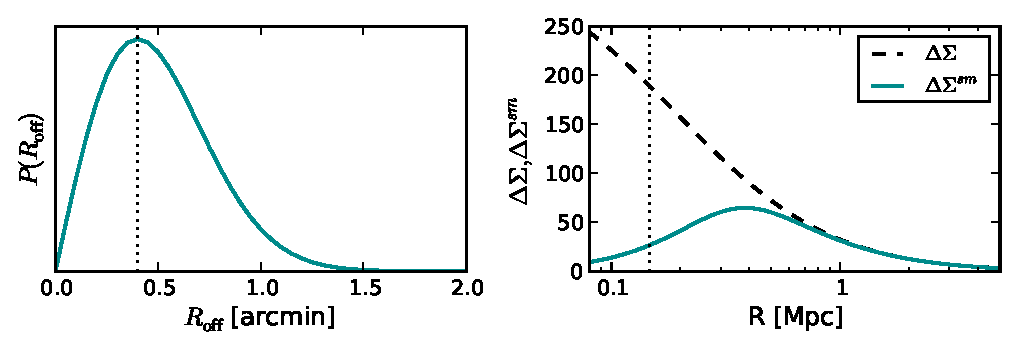
\includegraphics[scale=1.0]{plots_ch4/PofRc_DeltaSigma_example.eps}
  \caption[Example of Miscentering Effect on Shear Profile]{This figure is an illustrative example of typical $\Delta\Sigma(R)$ and $\Delta\Sigma^{\rm sm}(R)$ profiles, to demonstrate the effects of cluster miscentring (Equations 7 -- 11) on measured shear density profiles. The left-hand panel shows a typical probability distribution of centroid offsets, $P(R_{\mathrm{off}})$, modelled via a 2D Gaussian with $\sigma_{\mathrm{off}}$ = 0.4 arcmin. The right-hand panel demonstrates the effect of this offset distribution on the measured shear profile (in vertical axis units of [$M_{\odot}$/pc$^2$]) of a fiducial halo of mass $M_{200}=10^{14} M_{\odot}$, located at $z=0.5$. The dashed black curve shows the perfectly centred $\Delta\Sigma(R)$ profile, and the solid blue curve shows the miscentred profile $\Delta\Sigma^{\rm sm}(R)$. In both panels, the vertical dotted line marks the location of the miscentring offset $\sigma_{\mathrm{off}}$, to guide the eye in the comparison.}
\label{plot:miscentring}
\end{center}
\end{figure}


\subsubsection{Non-weak shear corrections}

The gravitational lensing observable is galaxy shapes. From these, we measure the reduced shear $g = \gamma / (1-\kappa)$ about the lens, where $\gamma$ is the true shear and $\kappa = \Sigma / \Sigma_{\mathrm{crit}}$ is the convergence \citep[as before, calculated using the NFW halo formalism in][]{Wright00}. At the innermost radii that we probe ($\sim$ 0.1 Mpc) the common weak lensing assumption that $g \approx \gamma$ may break down for the more massive clusters. We account for the difference between true and reduced shear using the correction factor from \citet{Johnston07}, which was worked out in detail in \citet{Mandelbaum06}. The differential surface mass density corrected for non-weak shear is given by:
\begin{equation}
\widehat{\Delta\Sigma} = \Delta\Sigma + \Delta\Sigma \ \Sigma \ \mathcal{L}_z,
\end{equation}
where $\mathcal{L}_z = \langle \Sigma_{\mathrm{crit}}^{-3} \rangle / \langle \Sigma_{\mathrm{crit}}^{-2} \rangle$ is calculated for each cluster redshift, using the full distribution of background galaxies satisfying the same redshift requirements outlined in Section \ref{sec:measure}. Similar to \citet{Leauthaud10}, we ignore any radial variations of $\mathcal{L}_z$, but do account for the variation with redshift, as our cluster sample spans a large $z$ range. The entire correction term $\Delta\Sigma \ \Sigma \ \mathcal{L}_z$ is negligible at all radii except for the innermost bin, where it typically makes up a few percent (at most $\sim$10\%) of the measured signal.

%----------------------------------------------

\subsection{Miscentring Formalism}
\label{sec:miscentring}

As was shown in \citet{Milkeraitis10}, 3D-MF does not always determine the exact correct centre for a galaxy cluster, and clusters may not always have a well-defined centre. This is a problem with all galaxy cluster finders and dealing with it properly involves understanding and quantifying its effects, such as including the uncertainty of the centre in calculations. The amplitude of measured shear profiles is absolutely dependent on the declared centre of the profile, so miscentring can potentially have a large impact on results. Offset cluster centres that are mistakenly modelled as being the true centres of the gravitational potentials will lead to underestimates in the inferred lens masses.

In our first analysis of the 3D-MF cluster candidates, we found modest evidence for cluster centroid errors \citep{Ford14}. However, that work relied on the lensing magnification technique, which is less sensitive to these effects than the shear, since magnification directly probes $\Sigma(R)$, while it is $\Delta\Sigma(R)$ that is more drastically reduced by a misplaced centre. See, for example, fig. 4 in \citet{Johnston07}, for a nice illustration of the comparative effect of miscentring on these two lensing profiles. 

In this work, we are able to directly quantify the presence of cluster miscentring by fitting for the offsets in our measurements of $\Delta\Sigma$. As will be shown in Section 4, we find that the best-fitting distribution of centroid offsets is in agreement with the following distribution based on simulations, which we assumed in \citet{Ford14}. 

The distribution of cluster offsets can be modelled as a two-dimensional Gaussian, by using a uniform angular distribution and the following radial profile:
\begin{equation}
P(R_{\mathrm{off}})=\frac{R_{\mathrm{off}}}{\sigma_{\mathrm{off}}^2}\ \mathrm{exp}\bigg[-\frac{1}{2}\bigg(\frac{R_{\mathrm{off}}}{\sigma_{\mathrm{off}}}\bigg)^2\ \bigg].
\end{equation}
Here, $R_{\mathrm{off}}$ is the projected offset of the 3D-MF derived galaxy cluster centre from the true galaxy cluster centre, and $\sigma_{\mathrm{off}}$ is the width of the distribution and one of the miscentring parameters which we fit to the stacked shear measurement. An example $P(R_{\mathrm{off}})$ curve is plotted in the left-hand panel of Figure \ref{plot:miscentring}, for $\sigma_{\mathrm{off}}$=0.4 arcmin. Note that we use physical units (e.g. Mpc) for most distances in this work, the exception being $\sigma_{\mathrm{off}}$ which we report in angular size (arcmin). The reason for this choice is that we believe a significant contribution to miscentring derives from 3D-MF's cluster characterization, which does not for example select a member galaxy as the centre (this choice of angular size is a matter of taste, since complex cluster physics certainly contributes to ambiguous halo centres). 

The effect of this offset distribution $P(R_{\mathrm{off}})$ is to reduce the ideal $\Sigma(R)$ to a smoothed profile \citep[see e.g.][]{Johnston07,George12}
\begin{equation}
\label{EQ:sigsmooth}
\Sigma^{\rm sm}(R)=\int_{0}^{\infty} \Sigma(R|R_{\mathrm{off}})\ P(R_{\mathrm{off}})\ \mathrm{d}R_{\mathrm{off}},
\end{equation}
which is illustrated in the right-hand panel of Figure \ref{plot:miscentring}. Equation \ref{EQ:sigsmooth} is an integration over all possible values of $R_{\mathrm{off}}$ in the distribution. The expression for the surface mass density at a single $R_{\mathrm{off}}$ is
\begin{equation}
\Sigma(R|R_{\mathrm{off}})=\frac{1}{2\pi}\int_{0}^{2\pi}\Sigma(r) \mathrm{d}\theta,
\end{equation}
where $r = \sqrt{R^2+R_{\mathrm{off}}^2-2RR_{\mathrm{off}}\cos(\theta)}$ and $\theta$ is the azimuthal angle \citep{Yang06}. From the smoothed $\Sigma^{\rm sm}(R)$ profile, we can obtain the smoothed shear profile:
\begin{equation}
\Delta\Sigma^{\rm sm} = \overline{\Sigma^{\rm sm}}(<R) - \Sigma^{\rm sm}(R)
\end{equation}
\begin{equation}
\overline{\Sigma^{\rm sm}}(<R) = \frac{2}{R^2} \int_{0}^{R} \Sigma^{\rm sm}(R')R'\mathrm{d}R'
\end{equation}

See \citet{George12} for a discussion of the effects of cluster miscentring on measured shear profiles. There are several different approaches in the literature for actually applying this formalism to data. For example, in some work authors apply the same smoothing to all clusters in a stack \citep{George12}, whereas others apply a two-component smoothing profile \citep{Oguri14}, or chose a uniform distribution of offsets instead of the Gaussian \citep{Sehgal13}. In our previous analysis of this cluster candidate sample, the magnification technique did not give significant constraining power for additional parameters, so we simply compared fits for both a perfectly centred and miscentred model, using estimates of $\sigma_{\mathrm{off}}$ obtained from running 3D-MF on simulations \citep{Ford14}. Both \citet{Johnston07} and \citet{Covone14} applied a combination of perfectly centred and miscentred haloes, thus fitting for the fraction of offset clusters in addition to the magnitude of the offset distribution $\sigma_{\mathrm{off}}$. We follow this latter approach in the current analysis.

As a caveat, we note that the degree of miscentring is fairly degenerate with the cluster concentration parameter, as both can have an effect on the amplitude of the inner shear profile. For example, we tried using the mass-concentration relation of \citet{Prada12}, which yields higher concentration for a given mass than the \citet{Dutton14} relation used here, and results in a best fit with larger centroid offsets. For the lower mass (richness) clusters this change is negligible, but for the most massive clusters in this study, the choice of concentration-mass relation can affect the miscentring fit parameters by as much as 40\%. Importantly, however, the best-fitting cluster mass is the {\it same} in both cases (within the stated 1$\sigma$ uncertainties). The degeneracy of cluster concentration and miscentring would be important to consider in a study seeking to constrain cluster mass-concentration relations. The measured concentrations will be biased low if cluster centroid offsets are significant and not fully accounted for.


%----------------------------------------------

\subsection{The Halo Model}
\label{sec:halomodel}
Weak lensing measurements are sensitive to the fact that structures in the Universe are spatially correlated. We account for this large scale clustering using the halo model, which provides a useful framework for modelling the clustered and complex dark matter environments that we probe in gravitational lensing studies. This phenomenological approach places all the matter in the Universe into spherical haloes, which are clustered according to their mass. Observables such as galaxies and clusters are considered biased tracers of the underlying dark matter distribution, with a bias factor that has been constrained in many numerical simulations \citep[e.g.][]{Mo96,Sheth99,Tinker10}. See \citet{Cooray02} for an extensive review of the halo model.

We follow an approach similar to \citet{Johnston07}, in considering a two-halo term in addition to the main NFW halo fit to our weak lensing shear measurement. Calculation of the two-halo term is identical to our approach in \citet{Ford14}, and we refer the reader there for explicit details. The two-halo term is proportional to a cluster bias factor which depends on mass, and for this we continue to use the $b(M)$ relation of \citet{Seljak04}. The full model including the two-halo term is:
\begin{equation}
\Delta\Sigma(R) = p_{\mathrm{cc}}\Delta\Sigma_{\mathrm{NFW}} +(1-p_{\mathrm{cc}})\Delta\Sigma_{\mathrm{NFW}}^{\rm sm} + \Delta\Sigma_{\mathrm{2halo}}
\label{modelEQ}
\end{equation}

The fraction of cluster candidates that is {\it correctly centred} on their parent dark matter haloes, $p_{\mathrm{cc}}$, is a parameter that we fit to the data. $p_{\mathrm{cc}}$ is a continuous variable, bounded between 0 and 1, fit separately for each stacked weak lensing measurement. Thus we have two cluster-centring-related parameters ($p_{\mathrm{cc}}$ and $\sigma_{\mathrm{off}}$), as well as one mass-related parameter ($M_0$), in the final modelling of the data.


%==========================================================================

\section{Galaxy Cluster Weak Lensing Shear Results}
\label{sec:results}

%----------------------------------------------
%RICHNESS-BINNED PLOTS
\begin{figure}
\begin{center}
%\vspace{2.cm}
  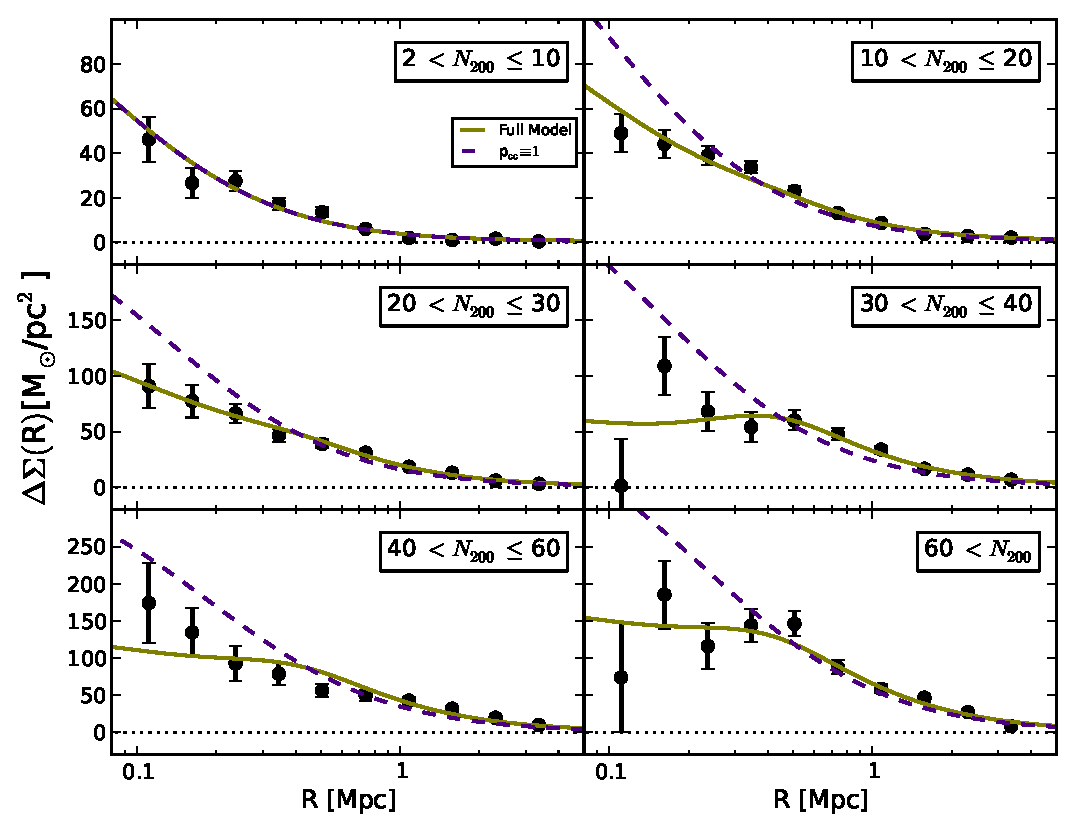
\includegraphics[scale=0.9]{plots_ch4/shearFit_panel_fcc0and1_slopeMN1p5_DuttonMaccio.eps}
  \caption[Shear for Richness-Binned Clusters]{Best-fitting models for each richness-binned stack of cluster candidates. The solid green curves are the best fits to the full model given by Equation \ref{modelEQ}. The dashed purple curves are the best-fitting models which assumes that every cluster centre identified by 3D-MF is perfectly aligned with the dark matter halo centre. With the exception of the lowest richness bin, where the best-fitting curves coincide, the perfectly centred model does not provide a good fit to the data at small $R$. Tables \ref{richbintable1} and \ref{richbintable2} summarize the results of both fits.}
\label{plot:nbinned}
\end{center}
\end{figure}

%M200 HISTS FOR N200 BINS
\begin{figure}
\begin{center}
%\vspace{1.2cm}
  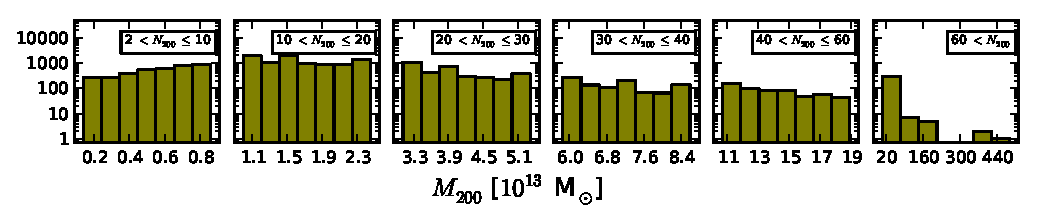
\includegraphics[scale=1.0]{plots_ch4/m200panels_NoGaps.eps}
  \caption[Cluster Mass Distributions for each Richness Bin]{The underlying distribution of cluster candidate masses, within each of the six richness bins in Figure \ref{plot:nbinned}, for the full miscentred model. Because the parameters fit to the shear measurements are the normalization of the mass-richness relation (Equation \ref{MNeq}) and the miscentring parameters $p_{\mathrm{cc}}$ and $\sigma_{\mathrm{off}}$, the full ({\it not binned}) set of cluster $N_{200}$ values are each converted to an individual cluster mass. We bin these masses for presentation in the above histograms only, but emphasize that the composite-halo modelling approach in this work treats every cluster candidate as having an individual mass (richness) and redshift. This figure is also a visual representation of the 3D-MF cluster mass function, as obtained from weak lensing shear.}
\label{plot:multimass}
\end{center}
\end{figure}


%----------------
%LANDSCAPE TABLES
\begin{landscape}

%TABLE FOR RICHNESS-BINNED PLOTS - FULL MODEL
\begin{table}
\centering
    \caption[Shear Results for Richness-Binned Clusters (Full Model)]{Details of the ``Full Model'' fits for the richness-binned measurements (Equation \ref{modelEQ}, green curves in Figure \ref{plot:nbinned}). This model has 7 degrees of freedom. We list the richness range selected, the number of cluster candidates in that bin, the shear detection significance, and the average richness and redshift of clusters in the bin. Fitted parameters include the centring-related parameters $p_{\mathrm{cc}}$ and $\sigma_{\mathrm{off}}$, and the normalization of the mass-richness relation $M_0$, from which the average mass in each bin $\langle M_{200} \rangle$ is derived. Note that the average mass given is not the value fit itself, but the average of all resulting masses fit using the composite-halo approach discussed in Section \ref{sec:nfw}. See Figure \ref{plot:multimass} for a summary of the mass distributions within each $N_{200}$ bin. Reduced generalized $\chi^2$ are given for each bin, and should be compared with the corresponding fits listed in Table \ref{richbintable2}, for the simple one-parameter model assuming perfect centres.}
    \begin{tabular}{llllllllll}
      \hline
      Richness & Clusters & Significance & $\langle N_{200} \rangle$ & $\langle z_l \rangle$ & $p_{\mathrm{cc}}$ & $\sigma_{\mathrm{off}}$ & $M_0 \left[ 10^{13} M_{\odot}\right]$ & $\langle M_{200} \rangle \left[ 10^{13} M_{\odot}\right]$ & $\chi^2_{\mathrm{red}}$ \\ \hline
      2 $<N_{200}\leq$ 10 & 3745 & 14.2$\sigma$ & 8 & 0.45 & 1.0$_{-0.2}$ & \---- & $2.4^{+0.9}_{-1.0}$ & $0.6^{+0.2}_{-0.3}$ & 2.1  \\
      10 $<N_{200}\leq$ 20 & 9034 & 22.8$\sigma$ & 15 & 0.63 & 0.5$\pm$0.1 & $(0.40^{+0.06}_{-0.2})'$ & $2.4\pm0.6$ & 1.6$\pm$0.4 & 2.3 \\
      20 $<N_{200}\leq$ 30 & 3409 & 25.6$\sigma$ & 24 & 0.67 & 0.5$\pm$0.1 & $(0.4^{+0.2}_{-0.1})'$ & $2.9\pm0.5$ & 3.9$\pm$0.7 & 0.8 \\
      30 $<N_{200}\leq$ 40 & 986 & 23.4$\sigma$ & 35 & 0.65 & 0.5$\pm$0.2 & $(0.4\pm0.1)'$ & $3.0\pm0.7$ & 7$\pm$2 & 2.6 \\
      40 $<N_{200}\leq$ 60 & 568 & 22.2$\sigma$ & 48 & 0.60 & 0.54$\pm$0.08 & $(1.3^{+0.5}_{-0.4})'$ & $3.6^{+0.8}_{-1.0}$ & $14^{+3}_{-4}$ & 0.3 \\
      60 $<N_{200}$ & 314 & 22.5$\sigma$ & 114 & 0.55 & 0.5$\pm$0.2 & $(0.4^{+0.2}_{-0.1})'$ & $1.6^{+0.4}_{-0.5}$ & 26$^{+6}_{-7}$ & 3.4 \\
      \hline
    \end{tabular}
\label{richbintable1}
\end{table}

%TABLE FOR RICHNESS-BINNED PLOTS - Pcc=1 MODEL
\begin{table}
\centering
    \caption[Shear Results for Richness-Binned Clusters (Perfectly Centred Model)]{This table is a companion to Table \ref{richbintable1}, giving details of the $p_{\mathrm{cc}} \equiv 1$ model fits for the richness-binned measurements (purple dashed curves in Figure \ref{plot:nbinned}). This model has 9 degrees of freedom. We list the richness range selected (the reader can refer to Table \ref{richbintable1} for the number of clusters, shear significance, and average richness and redshift). For this model, there is a single fit parameter, the normalization of the mass-richness relation $M_0$, from which $\langle M_{200} \rangle$ is derived (again see Figure \ref{plot:multimass} for the full distribution of masses in each richness bin).}
    \begin{tabular}{llll}
      \hline
      Richness & $M_0 \left[ 10^{13} M_{\odot}\right]$ & $\langle M_{200} \rangle \left[ 10^{13} M_{\odot}\right]$ & $\chi^2_{\mathrm{red}}$ \\ \hline
      2 $<N_{200}\leq$ 10 & 2.4$^{+0.4}_{-0.6}$ & 0.6$\pm$0.1 & 1.6  \\
      10 $<N_{200}\leq$ 20 & 1.8$\pm$0.2 & 1.2$\pm$0.2 & 4.8  \\
      20 $<N_{200}\leq$ 30 & 2.2$^{+0.2}_{-0.3}$ & 3.0$^{+0.3}_{-0.4}$ & 5.3  \\
      30 $<N_{200}\leq$ 40 & 2.4$\pm$0.3 & 5.5$\pm$0.8 & 4.4  \\
      40 $<N_{200}\leq$ 60 & 2.1$\pm$0.3 & 8$\pm$1 & 4.7  \\
      60 $<N_{200}$ & 1.4$\pm$0.2 & 23$\pm$3 & 4.4  \\
      \hline
    \end{tabular}
\label{richbintable2}
\end{table}

%TABLE FOR Z-BINNED PLOTS - FULL MODEL
\begin{table}
\centering
    \caption[Shear Results for Redshift-Binned Clusters (Full Model)]{Details of the ``Full Model'' fits for the redshift-binned measurements (green curves in Figure \ref{plot:zbinned}). This model has 7 degrees of freedom. We list the same bin properties and fits given in Table \ref{richbintable1}. The systematic errors listed on some cluster masses stem from uncertainties on the exact redshift of the cluster candidate. The fits in this table should be compared with the corresponding values in Table \ref{ztable2}, which represents the perfectly centred model.}
    \begin{tabular}{lllllllll}
      \hline
      Redshift & Clusters & Significance & $\langle N_{200} \rangle$ & $p_{\mathrm{cc}}$ & $\sigma_{\mathrm{off}}$ & $M_0 \left[ 10^{13} M_{\odot}\right]$ & $\langle M_{200} \rangle \left[ 10^{13} M_{\odot}\right]$ & $\chi^2_{\mathrm{red}}$ \\ \hline
      $z$ $\sim$ 0.2 & 1161 & 13.8$\sigma$ & 14 & 0.3$\pm$0.3 & $(0.4^{+0.3}_{-0.1})'$ & 3$\pm$1 & 2.3$^{+0.9}_{-1.0}\pm$0.4$^{\mathrm{sys}}$ & 0.6 \\
      $z$ $\sim$ 0.3 & 1521 & 15.7$\sigma$ & 17 & 0.8$^{+0.2}_{-0.3}$ & $(0.4^{+1}_{-0.4})'$ & 2.3$^{+0.7}_{-0.9}$ & 2.6$^{+0.8}_{-0.9}\pm$0.2 & 0.4 \\
      $z$ $\sim$ 0.4 & 2248 & 17.0$\sigma$ & 18 & 0.7$\pm$0.2 & $(0.4^{+0.3}_{-0.2})'$ & 2.6$\pm$0.9 & 3$\pm$1$\pm$0.1$^{\mathrm{sys}}$ & 0.8 \\
      $z$ $\sim$ 0.5 & 2935 & 20.2$\sigma$ & 18 & 0.8$\pm$0.2 & $(0.4^{+0.2}_{-0.3})'$ & 2.5$^{+0.6}_{-0.8}$ & 3.0$^{+0.7}_{-1.0}$ & 1.7 \\
      $z$ $\sim$ 0.6 & 2456 & 14.7$\sigma$ & 20 & 0.4$\pm$0.2 & $(0.4\pm0.1)'$ & 3$\pm$1 & 4$\pm$1 & 1.1 \\
      $z$ $\sim$ 0.7 & 2331 & 11.9$\sigma$ & 22 & 0.7$\pm$0.3 & $(0.4^{+0.6}_{-0.4})'$ & 2.1$^{+0.9}_{-1.0}$ & 3$\pm$1 & 0.8 \\
      $z$ $\sim$ 0.8 & 2364 & 8.7$\sigma$ & 22 & 0.2$\pm$0.2 & $(0.4\pm0.2)'$ & 3$^{+1}_{-3}$ & 4$^{+2}_{-3}$ & 1.9 \\ 
      $z$ $\sim$ 0.9 & 3040 & 6.8$\sigma$ & 19 & 0.6$\pm$0.4 & $(0.4^{+1}_{-0.4})'$ & 1.8$^{+0.8}_{-1.7}$ & 1.9$^{+0.9}_{-1.8}$ & 0.5 \\
      \hline
    \end{tabular}
    \label{ztable1}
\end{table}

%TABLE FOR Z-BINNED PLOTS - Pcc=1 MODEL
\begin{table}
\centering
    \caption[Shear Results for Redshift-Binned Clusters (Perfectly Centred Model)]{This table is a companion to Table \ref{ztable1}, giving details of the $p_{\mathrm{cc}} \equiv 1$ model fits for the redshift-binned measurements (purple dashed curves in Figure \ref{plot:zbinned}). This model has 9 degrees of freedom. For this model, there is a single fit parameter, the normalization of the mass-richness relation $M_0$, from which $\langle M_{200} \rangle$ is derived.}
    \begin{tabular}{llll}
      \hline
      Redshift & $M_0 \left[ 10^{13} M_{\odot}\right]$ & $\langle M_{200} \rangle \left[ 10^{13} M_{\odot}\right]$ & $\chi^2_{\mathrm{red}}$ \\ \hline
      $z$ $\sim$ 0.2 & 2.6$\pm$0.6 & 2.0$\pm$0.5$\pm$0.3$^{\mathrm{sys}}$ & 2.1  \\
      $z$ $\sim$ 0.3 & 2.1$\pm$0.4 & 2.4$\pm$0.4$\pm$0.2$^{\mathrm{sys}}$ & 0.4  \\
      $z$ $\sim$ 0.4 & 2.2$\pm$0.4 & 2.7$\pm$0.5$\pm$0.1$^{\mathrm{sys}}$ & 1.4  \\
      $z$ $\sim$ 0.5 & 2.2$\pm$0.3 & 2.7$\pm$0.4 & 1.6  \\
      $z$ $\sim$ 0.6 & 2.4$\pm$0.6 & 2.9$\pm$0.7 & 4.5  \\
      $z$ $\sim$ 0.7 & 1.9$^{+0.4}_{-0.5}$ & 2.4$^{+0.6}_{-0.7}$ & 0.8  \\
      $z$ $\sim$ 0.8 & 1.4$\pm$0.6 & 1.8$\pm$0.8 & 3.3  \\ 
      $z$ $\sim$ 0.9 & 1.3$\pm$0.6 & 1.4$\pm$0.6 & 0.6  \\
      \hline
    \end{tabular}
    \label{ztable2}
\end{table}

\end{landscape}
%----------------

\subsection{Fits to $\Delta\Sigma$}
\label{fits}

%MASS-RICHNESS PLOT
\begin{figure}
\begin{center}
%\vspace{0.5cm}
  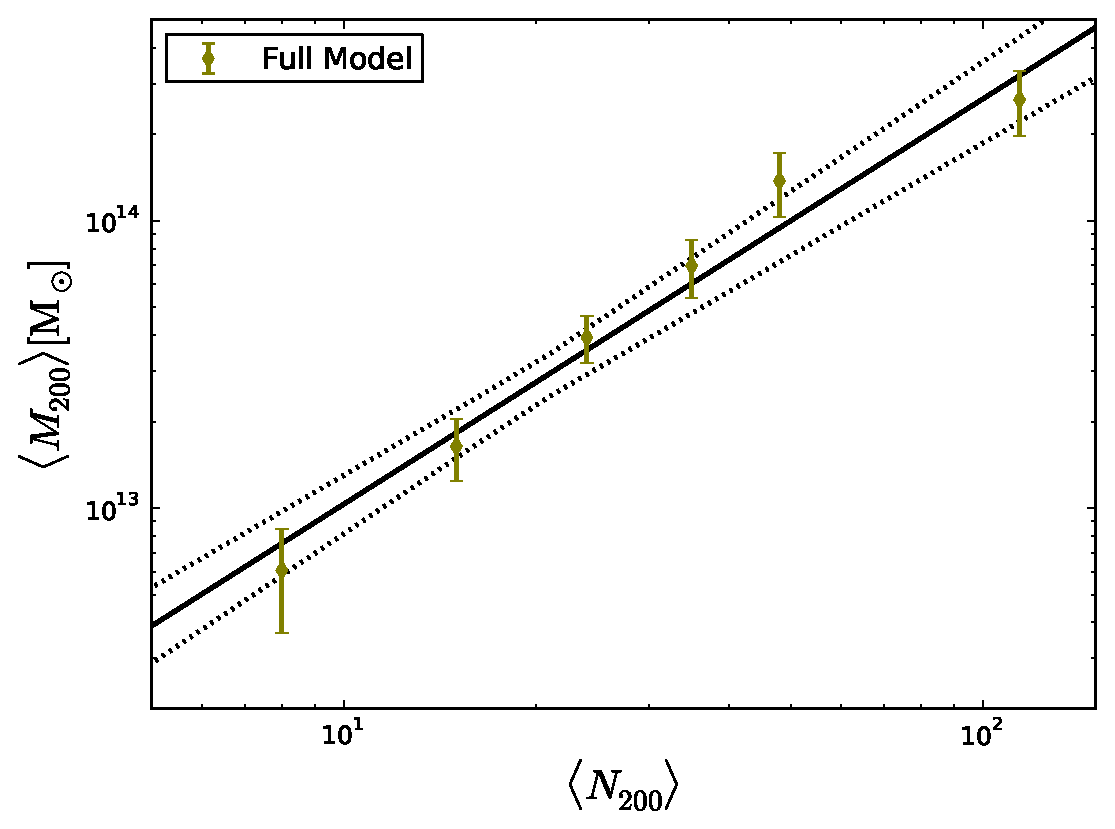
\includegraphics[scale=0.7]{plots_ch4/MassRich_shear_FullModelOnly_DuttonMaccio_IntrinsicScatter.eps}
  \caption[Mass-Richness Relation from Shear]{Power law best fit to mass-richness relation (Equation \ref{MNeq}) obtained from average masses measured for the individual $N_{200}$ bins in Figure \ref{plot:nbinned} and Table \ref{richbintable1}, for the full model which accounts for miscentring, and including the (very small) correction for intrinsic scatter. The dotted lines show the 1$\sigma$ limits on this relation. As discussed in Section \ref{sec:MN} the simple $p_{\mathrm{cc}} \equiv 1$ model, which assumes perfect cluster centres, yields the same slope, but a slightly lower overall normalization.}
\label{plot:massrich}
\end{center}
\end{figure}


We divide our cluster candidate catalogue into six richness bins, and measure the differential surface mass density as described in Section \ref{sec:measure}. The significances of the separate stacked measurements of $\Delta\Sigma(R)$ shown in Figure \ref{plot:nbinned} range from 14.2$\sigma$ to 25.6$\sigma$, calculated using the full covariance matrices to include correlation between radial measurement bins. Error bars are calculated as the square root of the diagonal of the covariance matrices. These values, along with details of the richness bins and fits are given in Table \ref{richbintable1}. This yields a total 3D-MF cluster shear significance of $\sim$54$\sigma$. 

In modelling the halo mass, we use a composite-halo approach, which allows for the fact that the cluster candidates in a given stacked measurement may have a range of individual masses and redshifts. We emphasize that instead of fitting a single average mass (and also avoiding a single effective cluster redshift), we actually fit to the normalization of the mass-richness relation, $M_0$. We convert the array of cluster $N_{200}$ values into masses with the equation
\begin{equation}
\label{MNeq1.5}
M_{200} = M_0 \left( \frac{N_{200}}{20} \right)^{1.5}.
\end{equation}

In each separate stacked weak lensing measurement, we keep the slope of this mass-richness relation fixed, to avoid over-fitting to each stack with parameters that are quite degenerate within a narrow cluster bin. The NFW mass of each individual cluster is given by Equation \ref{MNeq1.5}, with the fixed slope of 1.5 from \citet{Ford14}, which will be shown to be consistent with the global mass-richness relation, measured and discussed in Section \ref{sec:MN} of this current work. We note that because of the free normalization $M_0$, this approach does neither impose the form of the richness distribution (Figure \ref{plot:hists}) nor does it set a prior on the individual mass.

We fit the halo model given in Equation \ref{modelEQ} to the data, employing the downhill simplex method to minimize the generalized $\chi^2$, using the full covariance matrices estimated from bootstrap resampling. The results are displayed as the green curves in Figure \ref{plot:nbinned} (labelled ``Full Model''), and summarized in Table \ref{richbintable1}. The number of degrees of freedom for the model is 7 (10 radial bins minus 3 fit parameters). 

To emphasize the importance of cluster miscentring, we also plot the best-fitting model where $p_{\mathrm{cc}} \equiv 1$ (i.e. perfect cluster centres) for comparison. This is shown as the dashed purple curves in Figure \ref{plot:nbinned} (with a single fit parameter, $M_0$, this model has 9 degrees of freedom). Visual inspection reveals poor fits to the data at small radii for this model, and this fact is quantified by the reduced generalized $\chi^2$ statistic ($\chi^2_{\mathrm{red}}$) values in Table \ref{richbintable2}. These results imply that cluster centroiding is an important component in the modelling of the 3D-MF weak lensing shear mass profiles, especially at the high mass (richness) end. For the majority of the rest of this work we will focus our attention on the results of the full model, which accounts for offset cluster centres.

The ensemble of cluster masses that result from the composite-halo modelling approach are displayed in Figure \ref{plot:multimass}, where each panel represents a single stacked weak lensing measurement, congruent with Figure \ref{plot:nbinned}. This visual representation of the cluster mass function is largely distinct from the $N_{200}$ histogram in Figure \ref{plot:hists}, because these masses are dependent upon the mass-richness normalization, as well as the miscentring parameters, which are fit to the measurements.


%Z-BINNED PLOTS
\begin{figure}
\begin{center}
%\vspace{1cm}
  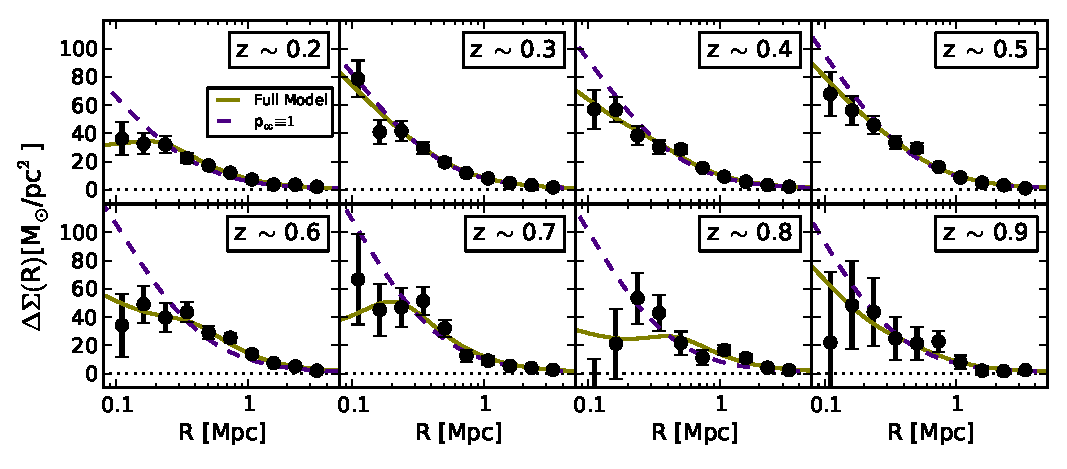
\includegraphics[scale=1.0]{plots_ch4/shearFit_zpanels_fcc0and1_slopeMN1p5_DuttonMaccio.eps}
  \caption[Shear for Redshift-Binned Clusters]{Best-fitting models for each stack of cluster candidates, this time binned in redshift. As in Figure \ref{plot:nbinned}, the solid green curves are the best fits to the full model given by Equation \ref{modelEQ}. The dashed purple curves are the best-fitting models which assumes that every cluster centre identified by 3D-MF is perfectly aligned with the dark matter halo centre. Tables \ref{ztable1} and \ref{ztable2} summarize the results of these fits.}
\label{plot:zbinned}
\end{center}
\end{figure}

%----------------------------------------------

\subsection{The Mass-Richness Relation}

\label{sec:MN}
The results of the previous section demonstrate a strong scaling of mass with richness. In Figure \ref{plot:massrich} we plot the average mass $M_{200}$ measured in each richness bin, as a function of richness $N_{200}$, and fit the power law scaling relation:
\begin{equation}
\label{MNeq}
M_{200} = M_0 \left( \frac{N_{200}}{20} \right)^\beta.
\end{equation}
This is similar to Equation \ref{MNeq1.5}, but the slope $\beta$ is now a free parameter, and the mass-richness normalization $M_0$ is fit across the full distribution of clusters. We note that the choice of $\beta=1.5$ in Equation \ref{MNeq1.5} does not have a significant effect on the $\beta$ measured here. Because of the degeneracy between $\beta$ and $M_0$ in each narrow cluster bin, a different choice of slope for the measurements in Section \ref{fits} still yields essentially the same mass estimates $M_{200}$, and thus the same global mass-richness relation.

Since galaxy clusters exhibit a natural intrinsic scatter between halo mass and richness (or other mass proxy), a bias in scaling relations can result if this scatter is ignored \citep{Rozo09a}. The idea here is that while galaxy clusters at a given richness will scatter randomly with regard to their average mass, because of the shape of the cluster mass function, the net effect is to scatter from low to high mass. This can lead to a biased mass estimate in a given richness bin, as well as affect the global result for the mass-richness relation. We correct for intrinsic scatter using the data itself, following a procedure inspired by \citet{Velander14}, which is as follows.

We first fit Equation \ref{MNeq} to the uncorrected raw mass estimates from each richness bin, and use this power law relation to assign an individual mass to each cluster, based on its value of $N_{200}$. We then draw many ``simulated'' clusters from the observed cluster mass function (i.e. the $N_{200}$ histogram in Figure \ref{plot:hists}), taking 1000 times as many ``simulated'' as observed clusters. We then scatter their masses by values drawn from a Gaussian in $\ln (M_{200})$, with width $\sigma_{\ln M|N}$, centred on the particular $N_{200}$. For the width of the intrinsic scatter, we use values estimated by \citet{Rozo09a} for the MaxBCG clusters in the Sloan Digital Sky Survey (SDSS). This is $\sigma_{\ln M|N} \sim 0.45$, which is the scatter in the natural logarithm of mass, at fixed richness.

The resulting mass estimates are then used to calculate the corrected arithmetic mean mass in each of the richness bins, which are plotted in Figure \ref{plot:massrich} and used to re-fit Equation \ref{MNeq}, yielding the final mass-richness relation reported below. The corrections applied to the mass estimates are at the sub-percent level, and therefore negligible compared to other sources of uncertainty in this work. Nevertheless, we include these small corrections when fitting for the mass-richness relation. We note that increasing $\sigma_{\ln M|N}$ up to the 95\% confidence limit reported by \citet{Rozo09a} still does not affect the conclusions drawn in this work. A glance at Figure \ref{plot:multimass} justifies the low-impact of the intrinsic scatter correction, as most richness bins do not exhibit a very strong slope, which would otherwise lead to a larger effect on average mass in each bin.

In this work we measure $M_0$ = $(2.7^{+0.5}_{-0.4}) \times 10^{13} M_{\odot}$ and $\beta$ = $1.4 \pm 0.1$ for the full model (Figure \ref{plot:massrich}), with a $\chi^2_{\mathrm{red}}$ of 0.9. For the perfectly centred model, we get $M_0$ = $(2.2 \pm 0.2) \times 10^{13} M_{\odot}$ and $\beta$ = $1.4 \pm 0.1$, with a $\chi^2_{\mathrm{red}}$ of 1.0. (Note that uncertainties are larger on parameters estimated from the full model, both here and throughout this work, since there are simply more parameters than the perfectly-centred model). These results demonstrate that not including the centroid uncertainty in our analysis would lead us to systematically underestimate the cluster masses as well as the mass-richness normalization. Section \ref{sec:magn} contains a thorough comparison of these results with our previous magnification measurements of these cluster candidates.


%----------------------------------------------

%Mo VS Z
\begin{figure}
\begin{center}
%\vspace{0.2cm}
  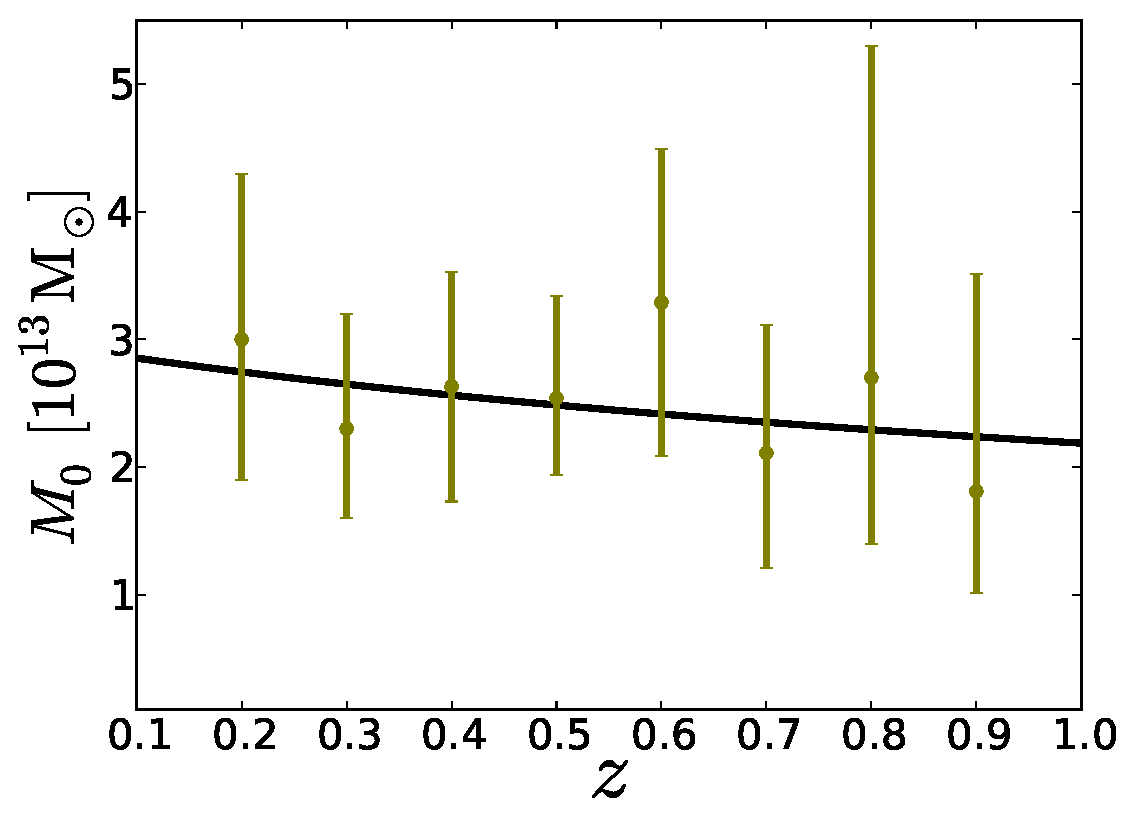
\includegraphics[scale=0.7]{plots_ch4/Mo_vs_z_DuttonMaccio_powerlaw.eps}
  \caption[Redshift Dependence of Mass-Richness Normalization]{Normalization of the mass-richness relation $M_0$ as a function of redshift $z$. The evidence for redshift evolution is not significant: the mildly negative slope is consistent with zero.}
\label{plot:MoVSz} %labels must be after caption
\end{center}
\end{figure}

\subsection{Results of Binning Clusters in Redshift}
We also investigate the weak lensing shear measurement of 3D-MF cluster candidates as a function of cluster redshift. 3D-MF sorts candidate clusters into bins of width $\Delta z \sim$ 0.1, so these are natural bin choices, and the same used in our previous analysis \citep{Ford14}. Figure \ref{plot:zbinned} shows the measurements and fits to $\Delta \Sigma$, with error bars again obtained from the covariance matrices (Section \ref{sec:measure}). The significance of the shear measurements reaches $\sim$ 20$\sigma$ at $z \sim$ 0.5, where there is an abundance of 3D-MF cluster candidates, and drops to $\sim$ 7$\sigma$ at the highest redshifts, where shear signal-to-noise is depleted. 

In Figure \ref{plot:zbinned} (similar to Figure \ref{plot:nbinned}), we plot the full model in solid green, and the perfectly centred model in dashed purple. Table \ref{ztable1} and Table \ref{ztable2} display the results and fit parameters for these two models, respectively. The measurements at lower redshifts have an additional systematic error listed, which stems from uncertainties on the cluster redshifts, due to the way the 3D-MF method slices in redshift space \citep{Ford14}. The 3D-MF cluster candidates are found to be quite similar in average mass across the range of redshift probed -- we consistently obtain measurements of a few $10^{13} M_{\odot}$. The best-fitting miscentring parameter $p_{\mathrm{cc}}$ varies somewhat erratically as a function of redshift, but the error bars are too large to infer any significance from this. The width of the offset distribution on the other hand remains squarely at $\sigma_{\mathrm{off}} \sim$ 0.4 arcmin. We discuss this result in relation to other cluster miscentring studies in Section \ref{sec:centres}.

We investigate possible redshift evolution of the mass-richness relation (given by Equation \ref{MNeq}) in Figure \ref{plot:MoVSz}, which shows the normalization of this scaling relation, $M_0$, as a function of redshift (with $\beta$ = 1.5 fixed), as listed in Table \ref{ztable1}. We fit a powerlaw relation of the form
\begin{equation}
\label{MoZeq}
M_0 (z) = M_0 (z=0) \cdot \left[ 1+z \right] ^{\gamma}.
\end{equation}
We find a normalization $M_0 (z=0) = (3.0 \pm 0.6) \times 10^{13} M_{\odot}$, and a powerlaw slope $\gamma = -0.4^{+0.5}_{-0.6}$. The slope is consistent with zero, so no significant redshift-evolution is detected for the 3D-MF mass-richness scaling relation.


%==========================================================================

\section{Discussion}

%----------------------------------------------

\subsection{Interpretation of the Results}

The 3D-MF clusters represent a wide range of halo masses and impose a significant shear signal on background galaxies. The measured $\Delta \Sigma$ profiles from different stacked subsamples of clusters yield an important glimpse at the state of the dark matter haloes. We fit a model that includes parameters designed to distinguish the fraction of well-centred versus offset haloes, and the width of the offset distribution. The latter is consistently measured to peak at an offset of $\sim$ 0.4 arcmin, except for the richness bin 40 $< N_{200} \leq$ 60, for which we find a larger best fit of 1.3 arcmin (this much larger offset is puzzling, and will require follow-up to determine whether it is physical or perhaps a spurious effect of overfitting). The fraction of clusters that are not correctly centred is generally about 50\% across richness bins, but has large error bars that do not allow us to distinguish interesting features at a statistically significant level. Nonetheless, we do find overall that the 3D-MF cluster halo profiles are better fitted by not enforcing perfect centroiding.

This study comprises several novel components, which will be discussed in more detail below. The large number of clusters, and the fact that 3D-MF does not assume anything about cluster galaxy colours, makes the uniqueness of the data set valuable in its own right.  Evolution of the normalization of the mass-richness relation across a wide span of redshift has only been constrained previously by \citet{EdoThesis12} and \citet{Andreon14}. The direct comparison between shear and magnification measured masses is a first for a cluster catalogue of this volume. There are several caveats to the implications of this work, notably the very likely presence of false-detections at the low-significance (low-richness) end of the cluster candidate spectrum.


%----------------------------------------------

\subsection{Comparisons of Cluster Catalogue Volume}

The most noteworthy aspect of the CFHTLS-Wide 3D-MF cluster catalogue is its sheer size. With over 100 cluster candidates per square degree (18056 clusters in 154 deg$^2$), spanning redshifts up to $z \sim$ 0.9, this compilation of cluster candidates is one of the most complete available. We encourage others to utilize this catalogue, available from \url{cfhtlens.org}, as there are an abundance of scientific investigations now possible with it. 

The current widest survey with a galaxy cluster catalogue is SDSS. The SDSS collaboration found 13823 galaxy groups and clusters spread over 7500 deg$^2$, using their maxBCG method \citep{Koester07}. This amounts to less than two clusters per deg$^2$, and is restricted to lower redshifts (0.1 $< z <$ 0.3). The maxBCG technique relies on finding potential bright galaxies and searching around them for the presence of a red sequence in colour-magnitude space (which would indicate the presence of red, elliptical galaxies, common in galaxy clusters). 

Interestingly, visual inspection of 3D-MF galaxy cluster candidates shows that the lower redshift clusters often do have a bright central galaxy, but this is less true at higher redshifts. It would be interesting to quantify this aspect in future work, especially when an opportunity presents itself to compare 3D-MF to other algorithms directly, by running both on the same optical data set. Galaxy clusters do not always have one brightest central galaxy, and if they do have one, it is not always exactly in the centre of the galaxy cluster, so comparing the biases of both methods could ultimately result in a more complete cluster list, or could potentially show the limitations of methods like maxBCG. 

Several cluster catalogues have been compiled in the CFHTLS-Wide. \citet{Durret11} used photometric redshift information to construct galaxy density maps in CFHTLS, building upon earlier work by \citet{Adami10} and \citet{Mazure07}. They found 4061 cluster candidates in the Wide fields, with masses greater than about 10$^{14} M_{\odot}$, spanning redshifts 0.1 $\le z \le$ 1.15. \citet{Shan12} used a 3D-lensing approach, with convergence maps and galaxy photometric redshifts, to detect 85 clusters at $\langle z \rangle \sim$ 0.36 in the W1 field of the CFHTLS-Wide.

\citet{Wen12} compiled an optical cluster catalogue from SDSS-III, using galaxy photometric redshifts and a friends-of-friends algorithm. They found an impressive 132684 clusters over 14000 deg$^2$ in a redshift range 0.05 $\leq z <$ 0.8. A recent cluster shear analysis was done by \citet{Covone14}, using the overlapping portion of the \citet{Wen12} catalogue, with the CFHTLenS shear catalogue. To date, this is the most complete cluster catalogue analysed in the context of CFHTLenS, but still the cluster density is $\leq$ 1/10th of that achieved with 3D-MF. A comparison of 3D-MF with the cluster catalogues compiled using these different techniques will be presented in a future analysis.

%----------------------------------------------

\subsection{Comparison with other Mass-Richness Relations}

The 3D-MF cluster finder presents us with a sample of cluster candidates which, like every other cluster-finder, are drawn from a somewhat unique distribution defined by its particular selection function. Despite the difficulties inherent to making exact comparisons between scaling relations measured on disparate cluster samples, we attempt a broad look at how the 3D-MF mass-richness scaling compares to other relations in the literature.

\citet{Wen09} defined a measure of richness $R$ for their SDSS clusters, which is somewhat similar to the $N_{200}$ used in this work. They counted all galaxies brighter than absolute magnitude $M_r \leq -21$, within a 1 Mpc radius and $\Delta z < 0.04(1+z)$. Converting their mass-richness relation to the form of ours (Equation \ref{MNeq}), they obtained a somewhat steeper slope $\beta \sim$ 1.9, and a higher normalization $M_0 \sim 2.5\times10^{14} M_{\odot}$ than the best-fitting models presented in this work ({\it Full Model}: $M_0 \sim 2.7\times10^{13} M_{\odot}$, $\beta \sim$ 1.4). We tried measuring richness for the 3D-MF clusters following the same prescription as \citet{Wen09}, but found the one-size-fits-all radius to be a serious limitation for our sample, since the 3D-MF cluster candidates span a wide range of masses and therefore characteristic radii. The resulting richness estimates had greatly enhanced scatter and did not scale well with mass at the more massive end of the cluster catalogue.

In a follow-up paper, \citet{Wen12} defined a new richness $R_{L*}$ -- the total r-band luminosity within $R_{200}$ in units of $L_{\odot}$. For the portion of clusters with previously measured masses (weak lensing or X-ray), a scaling between the radius $R_{200}$ derived from these masses and the luminosity within 1 Mpc was measured, and this was used to estimate radii for calculating $R_{L*}$ for the full sample of 132684 clusters. For the subsample with existing mass estimates, \citet{Wen12} found a mass-richness relation with normalization $M_0 \sim 1.1 \times 10^{14} M_{\odot}$ and slope $\beta \sim$ 1.2 (again converting to the form of our Equation \ref{MNeq}). \citet{Covone14} measured weak lensing masses for 1176 of the clusters from \citet{Wen12}, which overlapped with CFHTLenS. They found a very similar mass-richness scaling, with $M_0 \sim 10^{14} M_{\odot}$ and $\beta \sim$ 1.2. 

The mass-richness slope of the 3D-MF cluster candidates sits squarely between the results of \citet{Wen09}, using the $R$ richness, and \citet{Wen12} and \citet{Covone14}, which used the $R_{L*}$ measure. The 3D-MF normalization is lower than the other cluster catalogues, which could partly be a result of 3D-MF detecting more lower mass clusters missed by other finders. However, the different definition of richness, namely the fainter limit on galaxies contributing to $N_{200}$, means that the same mass cluster will have a larger measured richness in this work, implying a lower mass-richness normalization. Finally, the presence of false detections in the 3D-MF catalogue (estimated from simulations to be at the level of $16-24$\%) would certainly bias the mass estimates low.

\citet{Johnston07} used a quite different definition of richness for the maxBCG clusters, counting only red-sequence galaxies brighter than 0.4$L_*$, within an $R_{200}^{\rm gals}$ that was estimated from the number of galaxies within 1 Mpc \citep[following a prescription in][]{Hansen05}. Weak lensing masses were used to find a normalization $M_0 \sim 1.3 \times 10^{14} M_{\odot}$ and slope $\beta \sim$ 1.3. \citet{Rozo09b} created updated richness estimates of the maxBCG clusters by applying an improved colour modelling of cluster members, and allowing individual cluster radii to vary until the scatter between richness and X-ray luminosity was minimized.

\citet{Andreon10} defined a measure of richness for the Cluster Infall Regions in SDSS catalogue, for which masses $M_{200}$ and radii $R_{200}$ were already available (from application of the caustic technique). They studied a sample of 53 low-redshift clusters, in the range $0.03 < z < 0.1$, and their $N_{200}$ included all red galaxies brighter than $M_V = -20$ within the radius $R_{200}$. In a follow-up analysis they measured a tight mass-richness scaling relation with normalization $M_0 \sim 1.4 \times 10^{11} M_{\odot}$ and slope $\beta \sim 2.1$ \citep{Andreon12}.

The addition of the galaxy colour information in the richness estimate of the previous three examples, in particular, creates difficulty in drawing meaningful comparisons between their mass-richness scaling relation and the 3D-MF scaling relation. We emphasize that the value of any mass-richness relation is limited to the particular cluster sample for which it was derived, which in turn depends on the cluster-finding algorithm and details of the survey on which the catalogue was compiled. As discussed in \citet{Rozo09b}, the simple fact that estimates of richness are readily available in an optical cluster survey, and that they can be applied to clusters of virtually any mass, nevertheless makes richness a worthwhile parameter to measure. So although richness has many different definitions, and some unavoidable scatter in its scaling relations with various cluster mass estimates, it remains a useful tool for characterizing galaxy clusters. 

%----------------------------------------------

\subsection{Comparisons with other Cluster Centroid Analyses}
\label{sec:centres}
We find the distribution of centroid offsets to be well characterized by a Gaussian of width $\sigma_{\mathrm{off}} \sim$ 0.4 arcmin,\footnote[2]{For comparisons, 0.4 arcmin $\sim$ 147 kpc at redshift 0.5} and that this miscentring has an effect on a significant portion of the candidate clusters (up to $\sim$ 80\% of them are affected, see Table \ref{richbintable1}). Interestingly, previous studies applying 3D-MF to simulations yielded an average $\sigma_{\mathrm{off}}=0.40 \pm 0.06$ arcmin \citep[see Figure 1 in][]{Ford14}, which is easily consistent with the best-fitting offset measured on the real 3D-MF cluster candidates in this work.

%MAGNIFICATION COMPARISON PLOT
\begin{figure}
\begin{center}
%\vspace{1cm}
  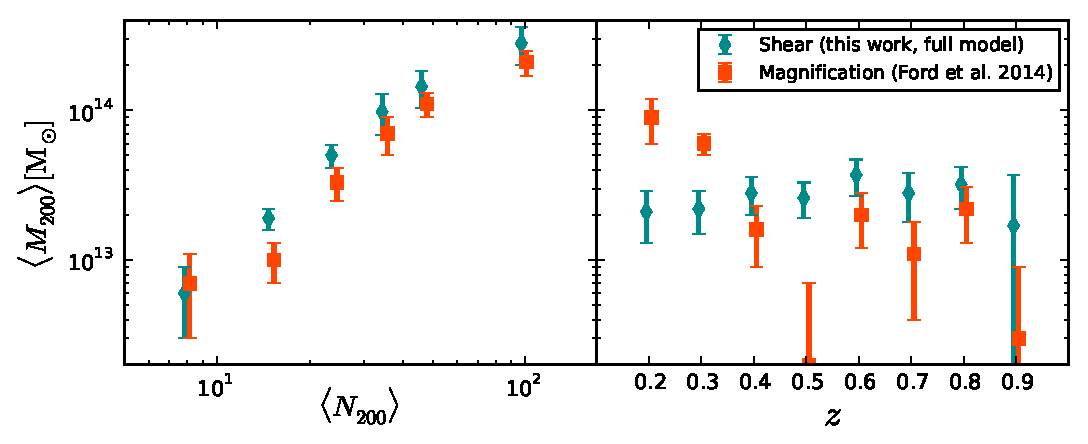
\includegraphics[scale=0.9]{plots_ch4/shearVSmag_N200_z.eps}
%\vspace{0.2cm}
  \caption[Comparison of Magnification and Shear Masses]{Here we compare the mass measurements obtained for the 3D-MF cluster candidates using weak lensing shear (i.e. this work) with the results obtained measuring the masses with the lensing magnification technique \citep[the $N_{200}$ estimates from that work, ][are used in this plot for the purposes of comparison]{Ford14}. The first panel compares mass measurements when cluster candidates are binned in richness $N_{200}$, and the second panel shows the redshift $z$ binning. Bins are identical for magnification and for shear, but the points are slightly offset horizontally for clarity. Blue diamonds represent the shear, and orange squares are for magnification.}
\label{plot:magshear}
\end{center}
\end{figure}

The maxBCG clusters were found to have centroid offsets around 0.42 $h^{-1}$Mpc, based on simulations \citep{Johnston07}, which is several times larger than the ones measured for the 3D-MF cluster candidates. There were large uncertainties associated with the probability of a cluster having a correct centroid selected, but this was determined to be approximately $\ge$50\% \citep[see Figure 5 in][]{Johnston07}, which is similar to $p_{cc}$ found in this work. \citet{George12} performed a miscentring analysis of X-ray groups in the COSMOS field. They found offsets of $\sim 20-70$ kpc, for different candidate centres, which are smaller than measured for 3D-MF clusters. 

It is worth noting that candidate cluster centres that are coincident with a member galaxy have been found to better trace the halo's centre of mass, relative to other types of centroids such as X-ray, or various weighted centres of galaxy positions \citep{George12}. See also \citet{Bildfell08} for a study of massive X-ray clusters. 3D-MF centres (peaks in the likelihood map) do not necessarily coincide with a cluster galaxy member, so future work should investigate various possible candidate centres to find the one that best traces the centre of mass for 3D-MF cluster haloes.

%----------------------------------------------

\subsection{Comparison with Magnification Results}
\label{sec:magn}

One of the most interesting aspects of this work is the direct comparison between magnification and shear mass estimates, which is now made possible in the context of a very large lens sample. Prior to this work, the only observational magnification--shear direct cluster mass comparison in the literature was \citet{Ford12}. That study demonstrated a 1$\sigma$ consistency between masses measured with the two techniques, but applied to a small sample of just 44 galaxy groups, so any trends in cluster size or redshift were unable to be explored. \citet{Huff14} compared magnification and shear masses for SDSS galaxy lenses, using a different and novel approach to measuring lensing magnification, and found mass profiles to be within a factor 3 of agreement.

Important work related to the {\it joint} analysis of shear and magnification has been developed in \citet{Umetsu11} and \citet{Umetsu13}. \citet{Umetsu14} combined shear and magnification to measure the mass profiles of 20 massive X-ray-selected clusters. This work demonstrated that the geometric mean mass of the shear+magnification measurement was consistent with the shear-only measurement, but did not show magnification results on their own. Earlier work in \citet{Umetsu11} compared the signal-to-noise of the magnification and shear, but did not present mass estimates from separate analyses. 

In this work we exploit the volume of the 3D-MF cluster catalogue to fully compare masses determined with each of the independent techniques, as a function of both candidate cluster richness and redshift. The findings are summarized in Figure \ref{plot:magshear}. For consistency in the comparison, this plot uses the original $N_{200}$ estimates from \citet{Ford14}, so that the cluster candidate stacks in each richness bin are identical. Also, in this section only, we use the mass-concentration relation of \citet{Prada12}, in identical fashion to the magnification work. The \citet{Prada12} relation is in excellent agreement with recent measurements by \citet{Covone14} of the masses and concentrations of a cluster sample in CFHTLenS, although it is in tension with other measurements such as \citet{Merten14}. 

The left-hand panel of Figure \ref{plot:magshear} displays the results when 3D-MF cluster candidates are stacked across all redshifts. The average of the composite-halo masses fit to each stack is comparable between the two methods, but the magnification estimates are systematically lower than the shear estimates. This yields a mass-richness normalization which is about 2$\sigma$ higher for the shear method, although the slope of the relation recovered with the two techniques is essentially identical. The magnification measurements yielded $M_0 = (2.2 \pm 0.2) \times 10^{13} M_{\odot}$ and $\beta = 1.5 \pm 0.1$ \citep[see the miscentred model in][]{Ford14}, while the shear measurements here give $M_0 = (3.1 \pm 0.5) \times 10^{13} M_{\odot}$ and $\beta = 1.5 \pm 0.2$. We note that the mass-richness relation parameters obtained from the shear measurements in Figure \ref{plot:magshear} are consistent within 1$\sigma$ with the new mass-richness parameters obtained with shear in Figure \ref{plot:massrich} and discussed in Section \ref{sec:MN}. We reiterate that the slight difference between the shear measurements in Figures \ref{plot:massrich} and \ref{plot:magshear} is due to a recalibration of the cluster $N_{200}$ estimates (see Section \ref{3DMF}) and a different choice of mass-concentration relation.

It is important to note that in both of the aforementioned magnification studies \citep{Ford12,Ford14}, the background source sample is completely distinct from the background sources used to measure shear. Indeed, both magnification results used magnified Lyman-break galaxies, which are point-like sources whose negligible apparent size would not permit a measurement of the shear. In this sense, the magnification results are largely independent from the shear measurements to which they are compared, having only the lens population in common. We note that alternative methods of measuring magnification using source size information would instead tend to use the same source sample employed for measuring shear.

The comparison becomes more interesting as a function of redshift, shown in the right-hand panel of Figure \ref{plot:magshear}. Here we see that the shear-measured average mass of cluster candidates does not vary as a function of redshift, while the magnification masses fluctuate. In \citet{Ford14}, we discussed this behaviour of the magnification signal, but without an alternative mass determination were not able to conclude whether this variation communicated an intrinsic property of the 3D-MF cluster candidates, or was an artefact of the magnification measurement. We are still unable to say with certainty whether the masses of the 3DMF cluster sample truly are constant or evolving across the redshift range, as suggested by the conflicting shear and magnification measurements. Here, we discuss several possible reasons for these discrepant redshift-binned results. 

First of all, the distributions of richness values for the separate $z$ slices are very similar, with the lower redshift slices containing relatively higher fractions of low-richness cluster candidates \citep[see Figure 7 in][]{Ford14}. So if (1) richness is a good estimator for mass, which it appears to be given the strong scaling, and (2) the mass-richness relation does not evolve strongly with redshift over the range $z \sim 0.5 \rightarrow 0.2$, then we would expect similar masses across this range, or for masses to actually decrease at lower redshift in concordance with the lower mean cluster $N_{200}$ (i.e. the opposite of the trend suggested by magnification).

As discussed in detail in \citet{Ford14}, at $z \sim 0.2-0.3$ the magnification measurement is expected to be affected by some low-$z$ contamination in the Lyman-break galaxy source sample. In that work we attempted to compensate for this effect by including a term in the modelling of the measured signal, to account for physical clustering where the populations overlapped. A crucial assumption was the actual fraction of contaminated sources, which was estimated using a cross-correlation technique with foreground galaxies (Hildebrandt et al., in preparation). If these fractions were biased low, then much of the physical clustering signal would have been interpreted as due to magnification, leading to mass estimates that were too high (at low-$z$).

Currently, we are also investigating the influence of several other systematic effects on our magnification measurements. In particular, we are studying how the varying depth and the varying seeing of the survey affect different lens and source samples, and how stellar contamination (or also just the light haloes of stars) and galactic dust can alter the magnification signal. This in-depth analysis of systematic effects will be presented in a forthcoming paper (Morrison et al., in preparation) and might provide additional insight into the apparent redshift dependence of the cluster magnification signal reported in \citet{Ford14}. Another possibility may be related to the masking effect of cluster galaxy members, which is survey dependent and can affect both magnification and shear measurements \citep{Simet14}. This sky obscuration could lead to our magnification masses being biased low, but our shear measurements should be robust because of the stringent criteria used for selecting background galaxies (Section \ref{sec:measure}).

In order for magnification to yield robust results that encourage its employment in the next generation of large surveys, this discrepancy needs to be addressed. Studies that compare shear and magnification measurements for large binned lens and source samples are crucial for teasing out these underlying systematics. 

%==========================================================================

\section{Conclusions}

This work has presented weak lensing shear results, measured at 54$\sigma$ significance, for a new catalogue of cluster candidates detected by the 3D-MF algorithm. 3D-MF is a three-dimensional advancement of older matched-filter techniques, which automatically searches wide and deep optical data for galaxy clusters across a range of redshifts. Given a sensible luminosity and radial profile, 3D-MF is able to search within data for a range of galaxy cluster masses. By construction, 3D-MF has allowed us to find lower mass cluster candidates (and groups) which other popular techniques, such as the red sequence and maxBCG, may not be capable of finding. 

3D-MF was run on the CFHTLS-Wide fields using galaxy photometric redshifts and $i'-$band data for cluster luminosity profiles, producing one of the largest and most complete cluster catalogues currently available. 18056 cluster candidates were detected with a significance $\ge 3.5$ and richness $N_{200} >$ 2, out to a redshift of 0.9 ($>$100/deg$^2$). Many of these cluster candidates are in the lower mass ranges (down to $\leq 10^{13} M_{\odot}$), which is notably a larger low mass sample than currently exists from deep, wide surveys in the literature, offering an enormous opportunity for further study. 

The CFHTLS-Wide 3D-MF catalogue was investigated to learn more about candidate cluster properties, such as masses and centroiding, as well as to follow up on previous results applying the less developed technique of lensing magnification to this cluster sample \citep{Ford14}. Shear profiles were measured around cluster candidates, which were stacked as a function of richness and redshift, and we focused on presenting composite-halo model fits to measurements of the differential surface mass density $\Delta\Sigma$. 

Careful consideration of potential miscentring of galaxy clusters by 3D-MF had to be taken into account in the analysis. We fit the data with smoothed shear profiles, $\Delta\Sigma^{\rm sm}$, that describe a cluster whose halo is offset from its assumed centre. The fraction of clusters that are affected by miscentring, as well as the probability distribution of the offsets, were both allowed to vary in the modelling. We found the inclusion of these parameters to significantly improve the $\chi^2$ of the cluster profile fits, relative to a perfectly centred model for $\Delta\Sigma$, which we also demonstrated for comparison. The stacked cluster shear measurements were well fitted by a model in which about half the clusters are affected by miscentring ($p_{\mathrm{cc}} \sim 0.5$), with the distribution of centroid offsets peaking at $\sim$ 0.4 arcmin.

The large sample of cluster candidates in this work allowed us to bin the shear measurements as a function of both richness and redshift. The average cluster candidate masses were found to be relatively constant with redshift, estimated at 2 to 4 $\times 10^{13} M_{\odot}$. The masses scaled strongly with richness, ranging from $\sim 6 \times 10^{12} M_{\odot}$ to $\sim 3 \times 10^{14} M_{\odot}$. We measured the normalization and slope of the mass-richness relation for the 3D-MF cluster candidates, finding $M_0$ = $(2.7^{+0.5}_{-0.4}) \times 10^{13} M_{\odot}$ and $\beta$ = $1.4 \pm 0.1$. The redshift dependence of the normalization $M_0 (z)$ was not significant, yielding a powerlaw slope in $(1+z)$ of $-0.4^{+0.5}_{-0.6}$. 

The masses of individual cluster candidates were found to range from a small group scale, with stacked average masses of less than $10^{13} M_{\odot}$, all the way up to a few very massive clusters, at several $10^{15} M_{\odot}$. Since the 3D-MF catalogue has not been followed up spectroscopically, we expect some fraction of false-detections (estimated between $\sim 16$ and $24$\% from simulations), which would lead to these mass estimates being biased low, and would especially affect the low-richness stacked measurements. We note, however, that the impact of false detections may be less severe than implied, if line-of-sight projections are significant. Chance alignments of low-mass structures would have a similar effect on a shear measurement (which probes surface mass density) as it would on an estimate of optical cluster properties like richness.

By design, we binned cluster candidates in an identical fashion to the previous magnification study \citep{Ford14}, and compared the results obtained. This is the first large study directly comparing the outcomes of magnification and shear on the same lens sample. When stacked across all redshifts, we found that the average masses derived within a given richness bin were similar (within 1$\sigma$), but magnification masses were systematically lower, yielding a 2$\sigma$ difference in the normalization of the mass-richness relation derived from the two techniques. The mass-richness slope was essentially identical for magnification and for shear. The comparison across redshift slices yielded very interesting insights into problems that may still exist for magnification. The fact that the shear-determined masses were roughly constant across redshift led us to conclude that the magnification measurement (using magnification-biased number counts of Lyman-break galaxy sources) may still suffer from residual systematics at low-$z$. Notably, however, this occurs at very predictable lens redshifts, so if one has accurate photometric redshift distributions for the sources, these contaminated redshift zones could potentially be avoided.

In future work, it would be interesting to apply various cluster finding algorithms to the {\em same} large data set in order to compare the capabilities of the finders, potentially increase the overall cluster sample and reduce its biases, or even just to compare how different search algorithms perform.  This could ideally lead to more complete and unbiased cluster samples. Current surveys, such as the Kilo-Degree Survey \citep{KiDS13}, the Subaru Hyper Suprime-Cam Project \citep{HSC10}, and the Dark Energy Survey \citep{DES05} for example, are large enough that cluster masses and concentrations will be measured quite accurately as a function of redshift and richness. The area of these surveys is an order of magnitude higher than the CFHTLS-Wide, and high precision cluster profiling will naturally continue to evolve alongside these surveys.

The CFHTLS-Wide 3D-MF galaxy cluster catalogue contains 18056 cluster candidates, over a wide range of mass and redshift, and is now publicly available at \url{cfhtlens.org}. We encourage others to make use of the rich science opportunities afforded by this catalogue. 

%==========================================================================









 %CFHTLenS Shear
%% The following is a directive for TeXShop to indicate the main file
%%!TEX root = diss.tex

\chapter{Conclusions}
\label{ch:conc}


%%%%%%%%%%%%%%%%%%%%%%%%%%%%%%%%%%%%%%%%%%%%%%%%%%%%%%%%%%%%%%%%%%%%%%
\section{Thesis Summary}
\label{sec:summary}

This thesis has presented novel results in the study of galaxy clusters through the use of weak gravitational lensing techniques. The scientific domain is the field of cosmology, which was discussed in \autoref{sec:Cosmology}. Cosmologists seek to understand the nature of the Universe on the largest scales -- its history, evolution, and fate, its large scale structure, and all the components of its energy density. This therefore requires knowledge of the matter distribution in the Universe, and how that has changed over time. 

Matter makes up a significant portion of the energy density of the Universe ($\sim30$\% today), and almost all of it is composed of dark matter, which appears to interact only through the gravitational force (see \autoref{sec:DM}). Matter was the dominant component of the Universe for much of its history -- from the time of matter-radiation equality, when the scale factor was just $a(t) \approx 2.9 \times 10^{-4}$, until the recent transition to the current dark energy domination \citep{PlanckXIII_15}. A very useful way to probe the dark matter distribution is through the study of gravitationally collapsed halos, such as those that house galaxies and galaxy clusters.

The specific importance and usefulness of galaxy cluster studies was discussed in \autoref{sec:Clusters}. The main goal, regarding galaxy clusters in this thesis, was to improve measurements of clusters masses, which are so important for both cosmological and astrophysical purposes. The methods employed in this thesis for improving galaxy cluster mass estimates consisted of two different and complementary approaches to weak gravitational lensing. Weak lensing is the subfield of gravitational lensing (see \autoref{sec:Lensing}), wherein light from background sources is subtly bent by gravitational potentials along its path, leading to the focusing and distortion of background galaxies. Unlike strong lensing, where lensing-induced features like giant arcs and multiple images are usually visible to the eye in images, weak lensing is not strong enough to produce obvious effects, but instead is used in a statistical sense, by averaging over many galaxies.

The first of the two weak lensing techniques, weak lensing shear, was explained in \autoref{sec:Shear}. Shear is ubiquitous in the weak lensing literature, and involves measuring slight distortions in image shapes. The second technique, magnification, was explained in \autoref{sec:Mag} and is the dominant focus of the thesis. Magnification is a relatively underused technique, compared to weak lensing shear, and its complementarity with the latter provided the motivation for this thesis research. Both types of weak lensing are statistical in nature, only measurable using many thousands of background galaxies behind many galaxy clusters or other gravitational lenses.  Magnification can be measured in several different ways, but the approach explored in this thesis uses the lensing-induced modifications to the source number densities that are detectable behind a gravitational lens.

The body of this thesis was composed of three published articles, sandwiched between an introduction to the relevant topics in \autoref{ch:Introduction}, and the current concluding chapter. These three peer-reviewed journal articles were all scientifically-led by the thesis author. The publication details can be found either in the Thesis Preface or in the Bibliography references for \citet{Ford12}, \citet{Ford14}, and \citet{Ford15}. 

\autoref{ch2} was comprised of the first magnification study applied to galaxy groups. Prior magnification studies were of galaxy lenses or of very massive (i.e. strongly lensing) clusters. This study yielded the first test of the technique on intermediate mass scales (several times $10^{13}\ {\rm M}_{\odot}$), and also included the first direct comparison between shear-measured masses and magnification-measured masses. These mass estimates were found to be in agreement, albeit with rather large uncertainties. The signal-to-noise from each technique was quantified and compared -- magnification yielded a 4.8$\sigma$ detection, whereas shear achieved 11$\sigma$.

In Chapters \ref{ch3} and \ref{ch4}, a much larger galaxy cluster sample was explored -- the \ac{3D-MF} cluster catalog from the \ac{CFHTLS}-Wide fields. This is one of the largest galaxy cluster catalogs that has been compiled (with over 18,000 clusters), notable containing many lower mass galaxy groups, and covering a wide range of redshifts, up to $z \sim 1$. Optimized with the goal of finding as many clusters as possible, the \ac{3D-MF} cluster finder produced a catalog that is 100\% complete for clusters with mass greater than $3 \times 10^{14}\ {\rm M}_{\odot}$ and 88\% complete above $10^{14}\ {\rm M}_{\odot}$ \citep[see \autoref{sec:3DMF4} or the original \ac{3D-MF} paper][for more details]{Milkeraitis10}. Compared with the small sample of X-ray selected galaxy groups analyzed in \autoref{ch2}, the \ac{3D-MF} clusters in \autoref{ch3} and \autoref{ch4} allow for superior signal-to-noise, even when the clusters are binned according to different attributes. This allows for important studies of clusters as a function of redshift and cluster richness (number of galaxies).

\autoref{ch3} focuses on the magnification signal of the \ac{3D-MF} clusters, which was detected at a significance of $9.7\sigma$. This chapter described the first magnification analysis with a large enough cluster sample to be able to bin as a function of richness \citep[however, note that the publication of this work was followed in quick succession by another magnification study of clusters and luminous red galaxies in the \ac{SDSS} by][]{Bauer14}. Using the richness-binned cluster mass estimates, a power-law scaling relation between cluster mass and richness was determined. This work compared the goodness of fit for two different types of cluster miscentering models -- the model assuming that \ac{3D-MF}'s selected cluster centers were perfectly accurate did not always fit the data as well as the model that assumed an offset distribution, with offsets based on simulations.

Additionally, the masses of clusters binned as a function of redshift were obtained, yielding unexpected variation of mass across redshift bins that had very similar richness distributions. This finding inspired further efforts to model a potential systematic effect for magnification -- physical overlap between lenses and sources in redshift space. Assuming some fraction of source contamination, the expected physical clustering signal was calculated and included in the models that were fit to the magnification signal. This was the first time such an approach had been attempted -- previous magnification studies had chosen to simply avoid interpreting any measurements in redshift regions where contamination is expected to be significant. Judgment regarding the success of this approach was withheld until the follow-up shear study of \autoref{ch4} was completed, in order to follow a semi-blind approach and avoid applying confirmation bias to the magnification results.

\autoref{ch4} paralleled the previous chapter in many respects. This included a shear analysis in the same spirit as the magnification one in \autoref{ch3}, using the publicly available shear measurements from \ac{CFHTLenS}. The binning of clusters was identical in each analysis, in order to produce a side-by-side comparison of the results from each of the two techniques. At 54$\sigma$, the shear signal measured from the cluster lenses is very strong, and this study was able to go beyond what was possible with magnification. In addition to measuring the mass-richness scaling relation, this analysis also searched for any evidence of this relation's evolution with cluster redshift. No significant evolution was detected, which is in line with other recent studies \citep{Andreon14}. 

This work also placed constraints on the \ac{3D-MF} cluster centroid offsets, which was an improvement over the magnification analysis of \autoref{ch3}, and was possible because shear is more sensitive to offset halos. Instead of comparing a perfectly centered model with an offset model, the shear analysis actually fit for the distribution of offsets, finding it to be reasonably well described by a Rayleigh distribution, peaking at a radial offset of $\sigma_{\rm off} \sim 0.4$ arcmin (although see \autoref{richbintable14} and \autoref{ztable14} for exact offset values, as well as other parameters). 

A thorough comparison of the results obtained for the \ac{3D-MF} clusters with other cluster analyses in the literature was presented in \autoref{sec:disc4}. Briefly, the slope of the mass-richness relation determined in this thesis was in line with other similar work \citep{Wen12,Covone14}, while the normalization is less easily compared, because it is highly sensitive to the definition of richness used for the sample (which varies widely in the literature). The cluster miscentering offsets measured in \autoref{ch4} of this thesis were intermediate between other results in the literature, which ranged from about half the radial offsets of \ac{3D-MF} \citep{George12} to several times larger than \ac{3D-MF} \citep{Johnston07}.

The research in this thesis pushed the limits of maximizing the extraction of weak lensing information to learn about cluster dark matter halos in our Universe. Two major analyses incorporating magnification information were completed, with some success, but also generated some doubt about the reliability of magnification when redshift contamination of sources is not well known. Prospects for improving the systematics-handling of future magnification studies will be discussed in \autoref{sec:future}. Regardless of any shortcomings of the technique, the undertaking of the detailed magnification studies in this thesis has added value to the weak lensing literature. This body of work provides a framework for accounting for systematic effects in magnification, and highlights issues and important considerations for future studies to build upon.


%%%%%%%%%%%%%%%%%%%%%%%%%%%%%%%%%%%%%%%%%%%%%%%%%%%%%%%%%%%%%%%%%%%%%%
\section{Final Conclusions}
\label{sec:conc}

The overall important findings produced by this thesis research can be summarized as a list of key take-away messages.
\begin{itemize}
\item Magnification can be successfully measured for galaxy groups and clusters, achieving up to half the signal-to-noise as the more commonly-measured shear technique (Chapters \ref{ch2}, \ref{ch3}, and \ref{ch4}).
\item It is possible to obtain consistent cluster mass estimates using weak lensing magnification and shear, at least when low-redshift contamination of sources (for magnification) is minimal (Chapters \ref{ch2} and \ref{ch4}).
\item The \ac{3D-MF} galaxy cluster catalog is publicly available as a result of this work (\autoref{ch4}).
\item The \ac{3D-MF} galaxy clusters exhibit a robust scaling between mass and richness (Chapters \ref{ch3} and \ref{ch4}).
\item The mass-richness scaling relation does not evolve significantly with redshift (\autoref{ch4}).
\item The cluster detection significance of the \ac{3D-MF} clusters scales with mass and can be used as an alternative mass proxy (\autoref{ch4}).
\item The miscentering of the \ac{3D-MF} clusters is significant (though less severe than for some other cluster catalogs) and must be accounted for to avoid biased lensing mass estimates (Chapters \ref{ch3} and \ref{ch4}).
\item The effects of cluster miscentering are degenerate with cluster concentration (\autoref{ch4}).
\item It is confirmed that magnification is highly sensitive to source contamination. Source redshifts and contamination fractions must be known very accurately, and underestimation may have devastating effects on recovered magnification-based masses (Chapters \ref{ch3} and \ref{ch4}).
\item Additional unconsidered systematic effects may plague magnification as well. Specific redshift intervals yielded anomalous magnification mass estimates that were difficult to blame on source contamination (\autoref{ch4}).
\end{itemize}

%%%%%%%%%%%%%%%%%%%%%%%%%%%%%%%%%%%%%%%%%%%%%%%%%%%%%%%%%%%%%%%%%%%%%%
\section{Future Prospects}
\label{sec:future}

There are a number of avenues of future research that could build upon the work in this thesis. The possibilities can be broken roughly into three major areas, which will each be discussed below. They include: galaxy cluster catalog comparisons for different cluster-finding techniques; galaxy cluster halo characterization and study; and the future of weak lensing magnification measurements in the era of upcoming large surveys. One common endeavor that will increase the progress of scientific results in general, will be encouragement of open science through making software and data products public and accessible for others to build upon.

The \ac{3D-MF} cluster catalog has many unique and important characteristics, and future work should compare the cluster sample to catalogs compiled using different cluster-finding techniques. For example, \ac{3D-MF} does not use any color information (aside from photometric redshifts) nor does it require a galaxy to be colocated with the cluster center. Many other cluster-finders rely on the red-sequence of member galaxies and assume that a luminous red galaxy lies at the center. This may allow \ac{3D-MF} to pick up less massive or evolved clusters, similar to our own Local Group. The careful comparison of different catalogs would help quantify real differences between the cluster samples recovered, and importantly would assist in removing false detections from the \ac{3D-MF} catalog (which are expected to be a significant fraction of the low-mass cluster candidates). Running the \ac{3D-MF} cluster-finder on the same optical data set, alongside other cluster-finders, and analyzing the different objects recovered, would also illuminate the overlap and complementarity of different techniques. Additionally, investigating the properties of galaxies in the \ac{3D-MF} clusters could be useful for constraining the halo occupation distribution, a framework for describing how galaxies occupy dark matter halos \citep{Coupon15}.

The issue of halo miscentering is interesting for a couple of reasons: (1) weak lensing mass estimates will be biased if miscentering is significant and not accounted for in modeling the lensing profile; (2) clusters that are poorly centered may represent a population of newly forming clusters, some of which might be undergoing mergers, and quantifying their presence and characteristics could be a useful probe of cluster and large-scale structure evolution. Future research should investigate the nature of the offset clusters in the \ac{3D-MF} catalog, to discover whether their centers are merely misidentified, or whether interesting cluster morphology exists. Additionally, alternative center definitions should be explored for the \ac{3D-MF} clusters. Side-by-side shear profile comparisons could demonstrate better center finding for some or all of the clusters, over the original definition employed by the \ac{3D-MF} algorithm.

More broadly, all weak lensing cluster studies need to consider the effects of miscentering. Justification should be given if the distribution of offsets is not accounted for in a weak lensing shear analysis. Studies that purport to measure cluster concentration should be careful to rule out miscentering, the effect of which mimics a low-concentration dark matter halo, by reducing the amplitude of the shear profile at small radii. 

Future magnification studies will need to carefully address the serious systemic effect of the contamination of background sources with objects that overlap with the low-redshift lens population. This can be approached either by improving redshift estimates for sources, so that a pure background sample can be obtained, or by simply avoiding regions of redshift overlap. Additional possible sources of systematics need to be quantified, and some work is being done in this regard by Hildebrandt et al. (private communication). Possible issues may include variations across the images in depth, atmospheric seeing, and contamination by the light halos of stars.

Within the next decade several important large astronomical surveys will begin collecting data. The \acf{LSST} is an 8.4-m telescope, currently under construction in Chile. Starting around 2021, \ac{LSST} will spend 10 years surveying 30,000 deg$^2$ of sky (nearly 200 times the area of \ac{CFHTLenS}) in 6 optical to infrared wavelength bands, providing unprecedented wide field data for weak lensing studies and many other astronomical pursuits \citep{LSST2.0}. \acs{Euclid} is a European Space Agency 1.2-m space-based telescope, planned for launch in 2020, with the goal of improving dark energy constraints. It will spend 6 years obtaining deep imaging of 15,000 deg$^2$ of sky, and weak gravitational lensing is one of the central focuses \citep{Euclid}. By performing tomographic weak lensing (redshift-binned weak lensing), the growth of structure and the influence of dark energy on the expansion will be measured. The \acf{WFIRST} is a NASA 2.4-m space-based telescope, planned for launch by 2024. Among its other scientific goals, \ac{WFIRST} will perform a weak lensing survey of 2,200 deg$^2$, employing six filters in the near-infrared wavelength range \citep{WFIRST}. 

Weak gravitational lensing is a common central focus of all major upcoming missions and surveys, as it has become an indispensable tool for probing the dark matter, geometry, and growth of structure in our Universe. Key questions that remain prominent in cosmology include the nature of dark matter and dark energy, and the complicated connection between baryonic physics and this dark sector. Gravitational lensing provides a means to accurately mapping the dark matter structures and distribution, and will continue to yield constraints on the dark matter particle self-interaction cross-section through the study of merging clusters \citep{DawsonThesis13,WittmanProposal13}. By measuring the redshift dependence of the cross-correlations of matter in the universe, the nature of dark energy -- as a cosmological constant or a more complex phenomena -- will be elucidated. The unique ability of gravitational lensing to measure total mass (including dark matter) is immensely important for improving models that seek to connect the state of visible matter -- various types of galaxies and the \ac{ICM} -- with environment and evolutionary history.

Magnification, despite some limitations discussed in this thesis, offers great benefits and additional opportunities for these surveys. Especially for ground-based surveys like \ac{LSST}, which will be affected by atmospheric seeing, the ability to use unresolved sources increases the number of gravitationally lensed galaxies that can be included in an analysis. A few simple calculations demonstrate the enormous improvements in signal-to-noise that will be possible for magnification with \ac{LSST}. Assuming that signal-to-noise scales roughly with the square root of the number of sources, which depends on survey area and limiting magnitude, we can project that the signal-to-noise for magnification with \ac{LSST} will be more than 100 times larger than for \ac{CFHTLenS}.\footnote{This estimate assumes that the source flux at limiting magnitude is inversely proportional to the square root of observing time, and time is proportional to number of sources detected, as in Equation 20 of \citet{Chang13}. Additionally, \ac{LSST} will be about 100 times larger area than \ac{CFHTLenS}, which will increase the number of sources by roughly that factor as well: \\ $\frac{(S/N)_{\rm LSST}}{(S/N)_{\rm CFHTLenS}} \sim \sqrt{\frac{18,000\ {\rm deg}^2}{171\ {\rm deg}^2}} \times 10^{-0.4(m_{\rm CFHTLenS} - m_{\rm LSST})} \sim 135$.\\ The first factor is the ratio of unmasked areas, the second gives the contribution from the relative limiting magnitudes of each survey. In reality, various factors will complicate this calculation, including telescope seeing, accuracy of galaxy redshifts, purity of the lens and source selection, among other observational and technical challenges associated with a ground-breaking new telescope like \ac{LSST}.}

Importantly, for any of these surveys, the opportunity to perform magnification studies at all is a free source of additional lensing information. Regardless of whether the final deliberation for these surveys is to improve contamination modeling, to use only unaffected redshift regimes, or even to focus on alternative measures of magnification using sizes or redshift distributions, magnification information can and will be exploited, because it is free information. The work contained in this thesis has played an important role in laying the foundation for future studies that will maximize the use of weak gravitational lensing survey data.


%%%%%%%%%%%%%%%%%%%%%%%%%%%%%%%%%%%%%%%%%%%%%%%%%%%%%%%%%%%%%%%%%%%%%%
\endinput
Any text after an \endinput is ignored.
You could put scraps here or things in progress.



%    3. Notes
%    4. Footnotes

%    5. Bibliography
\begin{singlespace}
\raggedright
\bibliographystyle{abbrvnat}
\bibliography{References}
%\bibliography{biblio}
\end{singlespace}

\appendix
%    6. Appendices (including copies of all required UBC Research
%       Ethics Board's Certificates of Approval)
%\include{reb-coa}	% pdfpages is useful here
\chapter{Supporting Materials}

This would be any supporting material not central to the dissertation.
For example:
\begin{itemize}
\item Authorizations from Research Ethics Boards for the various
    experiments conducted during the course of research.
\item Copies of questionnaires and survey instruments.
\end{itemize}


\backmatter
%    7. Index
% See the makeindex package: the following page provides a quick overview
% <http://www.image.ufl.edu/help/latex/latex_indexes.shtml>


\end{document}
